%
%  W/top - lost lepton subsection
%
\section{Concept of the lost-lepton background estimation}
The by far most important fraction of events in the search region leading to $e$ and $\mu$ with jets in the final state originates either from the decay of a \ttbar where $t\rightarrow b+W^+$ ($\bar{t} \rightarrow \bar{b}+W^-$) or from a \wpj event. Fig.~\ref{fig:lostlepton_feynman} shows typical Feynman diagrams for such events. The involved $W$ decays either directly to an $e + \nu_{e}$ or $\mu + \nu_{\mu}$ or via the intermediate state of a $\tau + \nu_{\tau}$. In the following only muons and electrons are meant by ''leptons'' if not stated otherwise.\\
 % which decays than further to an electron and neutrino or muon and neutrino. 
\begin{figure}[tbhn]
\begin{center}
\begin{tabular}{cc}
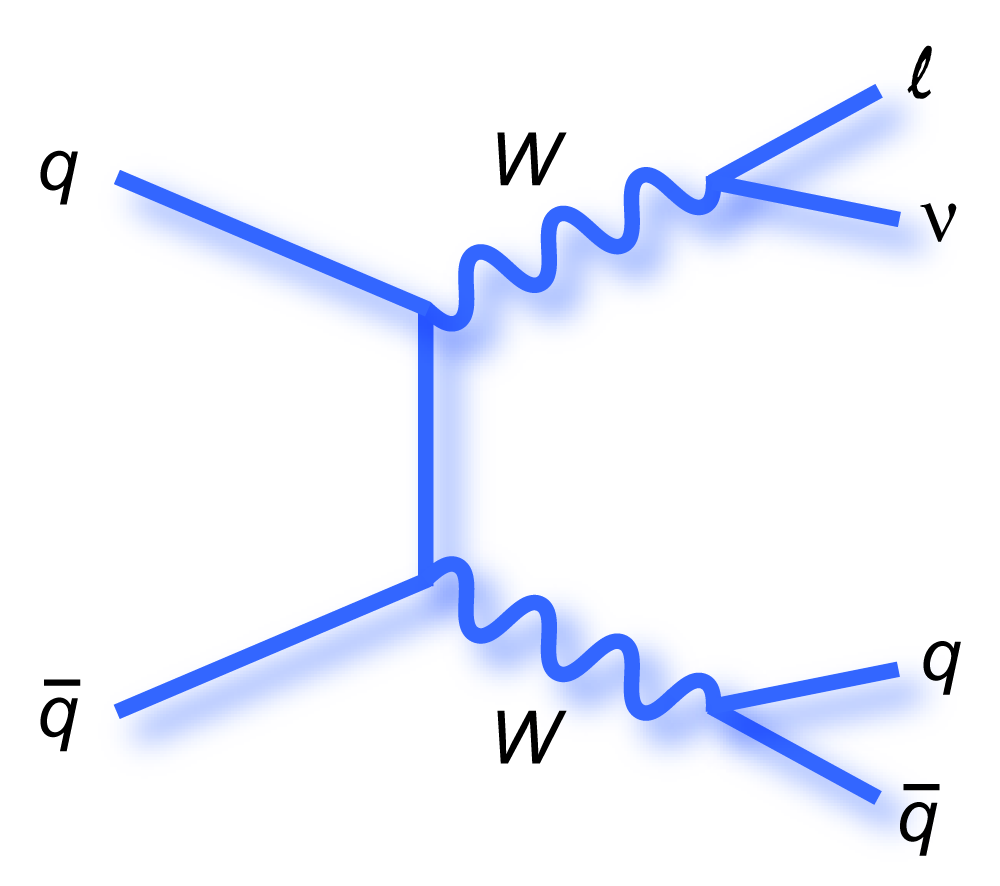
\includegraphics[width=0.49\textwidth]{lostlepton/plots/feynman_WW_lnuqq_bold_midblue.png}
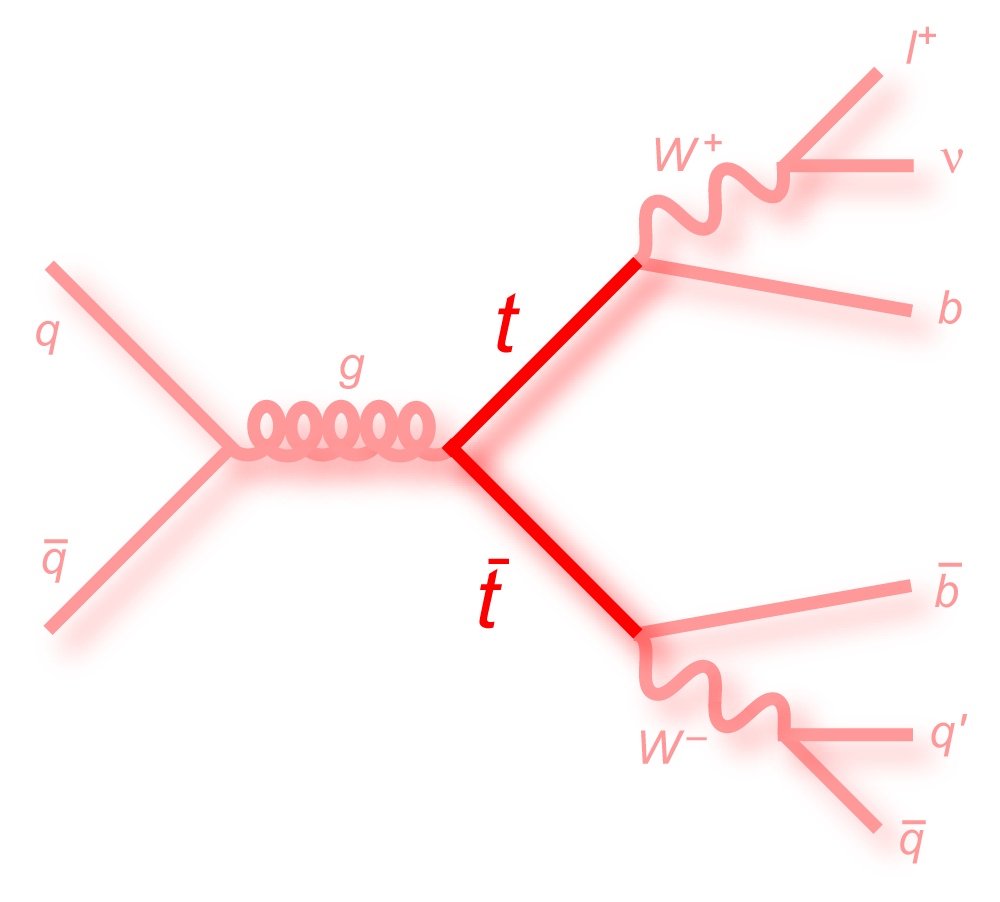
\includegraphics[width=0.49\textwidth]{lostlepton/plots/ttbar_feynman.png}\\
\end{tabular}
\end{center}
\caption{Feynman diagram for a typical \wpj decay on the left and a \ttbar decay on the right at the LHC\cite{tevatronPlots:2010}.}
\label{fig:lostlepton_feynman}
\end{figure}
The $\nu$ leaves the detector undetected leading to missing transverse energy. The lepton veto defined in Sec.~\ref{sec:event_selection} removes only events if leptons are within the detectors acceptance and fulfill the reconstruction and isolation criteria. The lost-lepton background arises when the lepton veto fails to identify a prompt lepton.\\
%The method which is described in this section is capable of predicting events with lost leptons, for very high \HT and \MHT regions. 
The background is estimated by a muon control sample (CS) which is reweighted according to the lepton identification (in)efficiency of the detector.
%The idea of predicting these lost-leptons is to selecting events which full fill the same kinematic cuts, except that they include exactly one well detected muon. This sample is called the control sample (CS), see Sec. \ref{sec:controlSample}. 
%The spectrum of the $\mu$ CS \pt is compared for the simulated events to the muons selected on data. Good agreement can be observed. The \pt of the muon also adds to the \HT and \MHT.
%The \pt of the muon, which can be seen in plot\ref{fig:CSmuonpt}, adds to the \HT and \MHT.\\
%The events of the CS are re weighting according to the (in)efficiency of the detector to reconstruct leptons. 
This idea holds when the event kinematics of the CS and the not detected leptons are similar, so that the background can be modeled by the CS. Extensive tests on simulated events have been performed to prove the methods capability of predicting lost leptons, see Sec.~\ref{sec:closure_test}.\\
All plots in this section labeled ''CMS Simulation'', ''CMS preliminary'' or ''CMS'' have been done by me, made public by CMS and can be found on the public twiki web page \cite{bib:TWiki:SUS12011}.

\section{The control sample}
\label{sec:controlSample}
The control sample (CS) includes events which pass the same kinematic cuts as the event selection (see Sec.~\ref{sec:event_selection}) but the lepton veto is inverted requiring exactly one well identified muon. The \pt of the muon is included in the \HT and \MHT calculation.\\
A small contribution comes from \ttbar decays to two leptons (dileptonic). These events enter the CS if only one lepton is lost. The case that one lepton is lost is twice as often than both are lost. The amount of lost leptons is therefore overestimated by a factor of two for the dileptonic decays. A selection on MC of events including one muon from dileptonic decays has been compared to the selection where two leptons are lost. The \mt cut discussed in Sec.~\ref{sec:event_selection} reduces the amount of dileptons in the CS to only 3\% of the total CS. These 3\% lead to an over-prediction of 1.5\% of the total prediction. The prediction is corrected for this.\\
Another minor contribution arises form diboson event and single top. The contribution has been found to be be less than 1.5\% of the total CS. This contribution is covered within the assigned uncertainty (see Sec.\ref{sec:uncertainties}).
Fig.~\ref{fig:CSmuonpt} and Fig.~\ref{fig:LostLepton_MuCS_data_MC} show the \pt, \HT and \MHT distribution of the CS selected from simulated \ttbar and \wpj events and data. Good agreement can be observed.
 %This proves that the assumption of no significant difference of the event kinematics between the CS to the lost lepton is reasonable. 

\begin{figure}[tbhn]
\label{fig:LostLepton_MuCS_data_MC}
\begin{center}
\begin{tabular}{c}
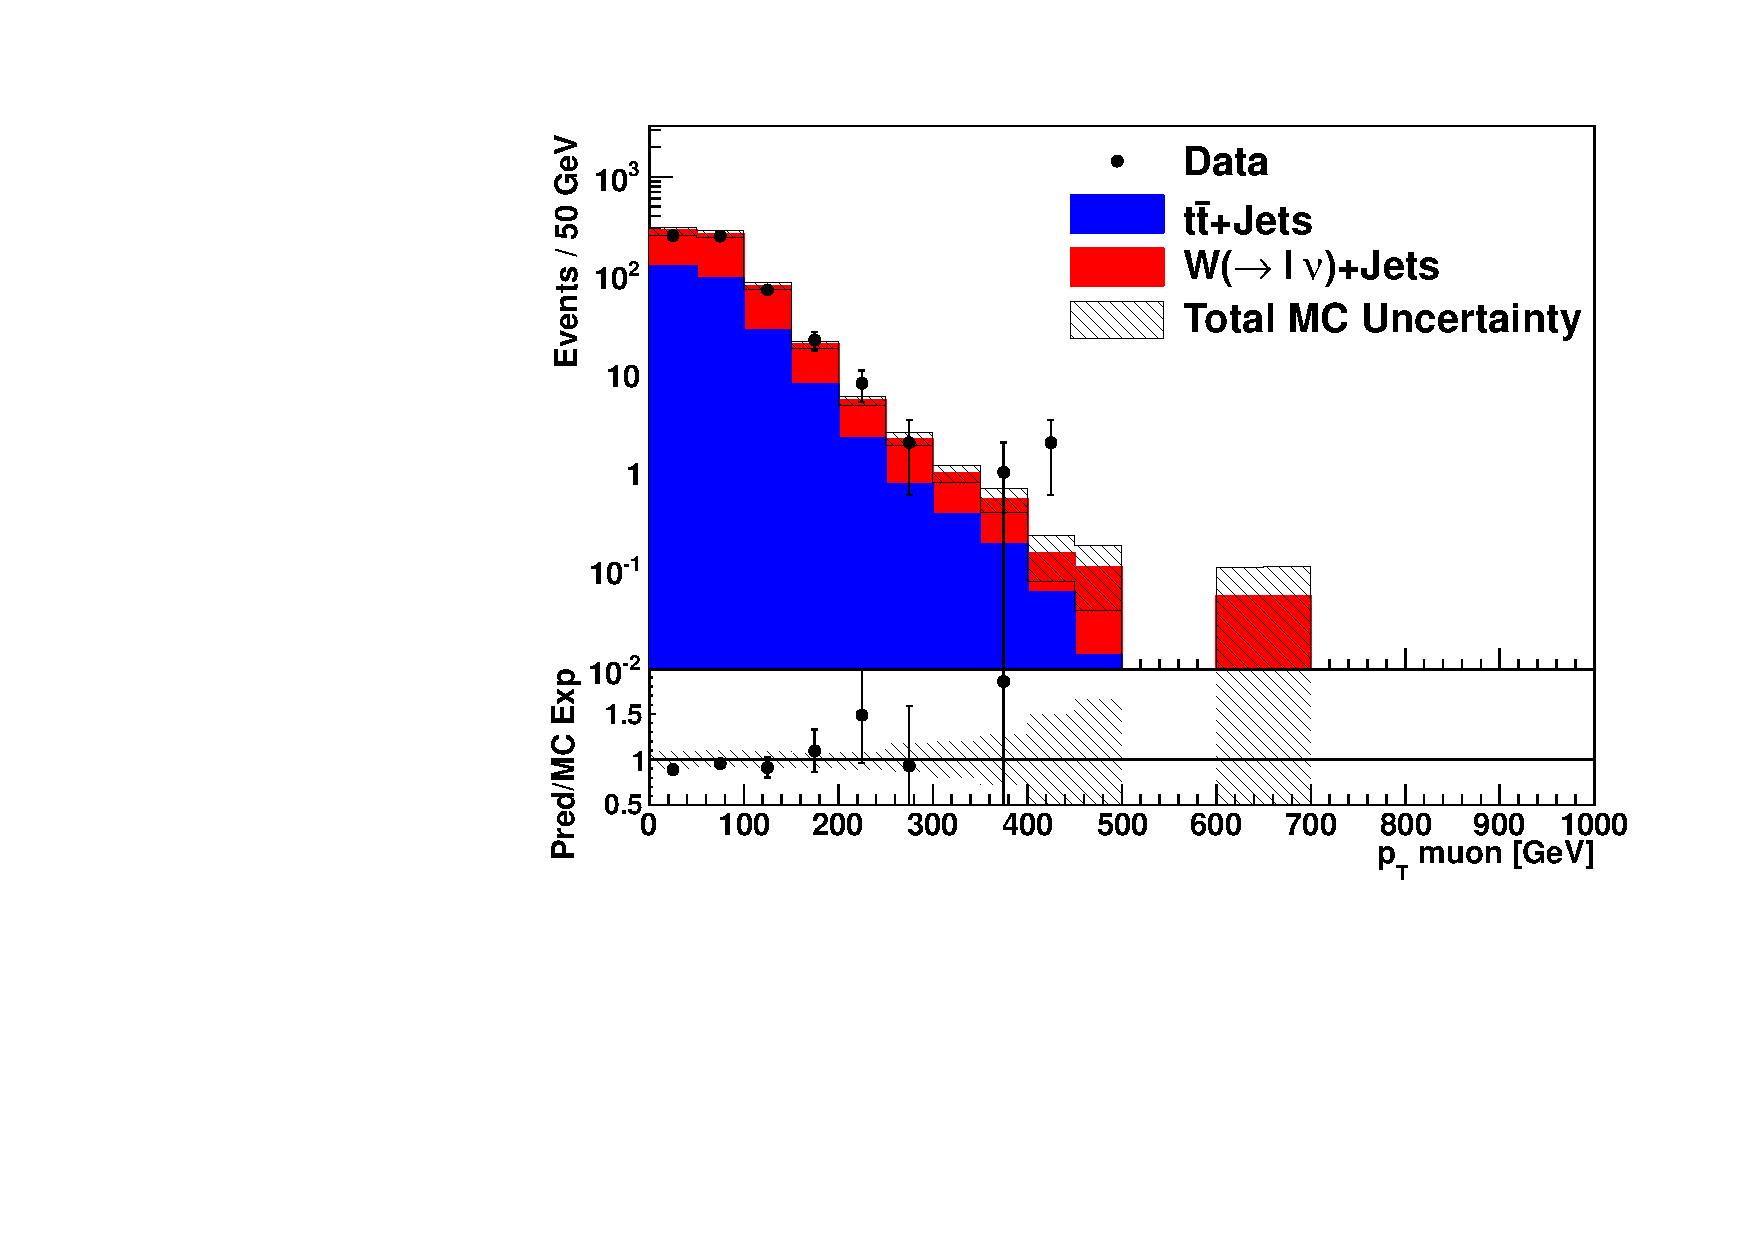
\includegraphics[width=0.90\textwidth]{lostlepton/plots/closure/CSMuonPT.pdf}
\end{tabular}
\end{center}
\caption{This plot shows a comparison of the $\mu$ control sample \pt spectrum selected on data corresponding to the full \lumi recorded 2011 and simulated \ttbar and \wpj events referred to as MC.}
\label{fig:CSmuonpt}
\end{figure}

\begin{figure}[tbhn]
\begin{center}
\begin{tabular}{cc}
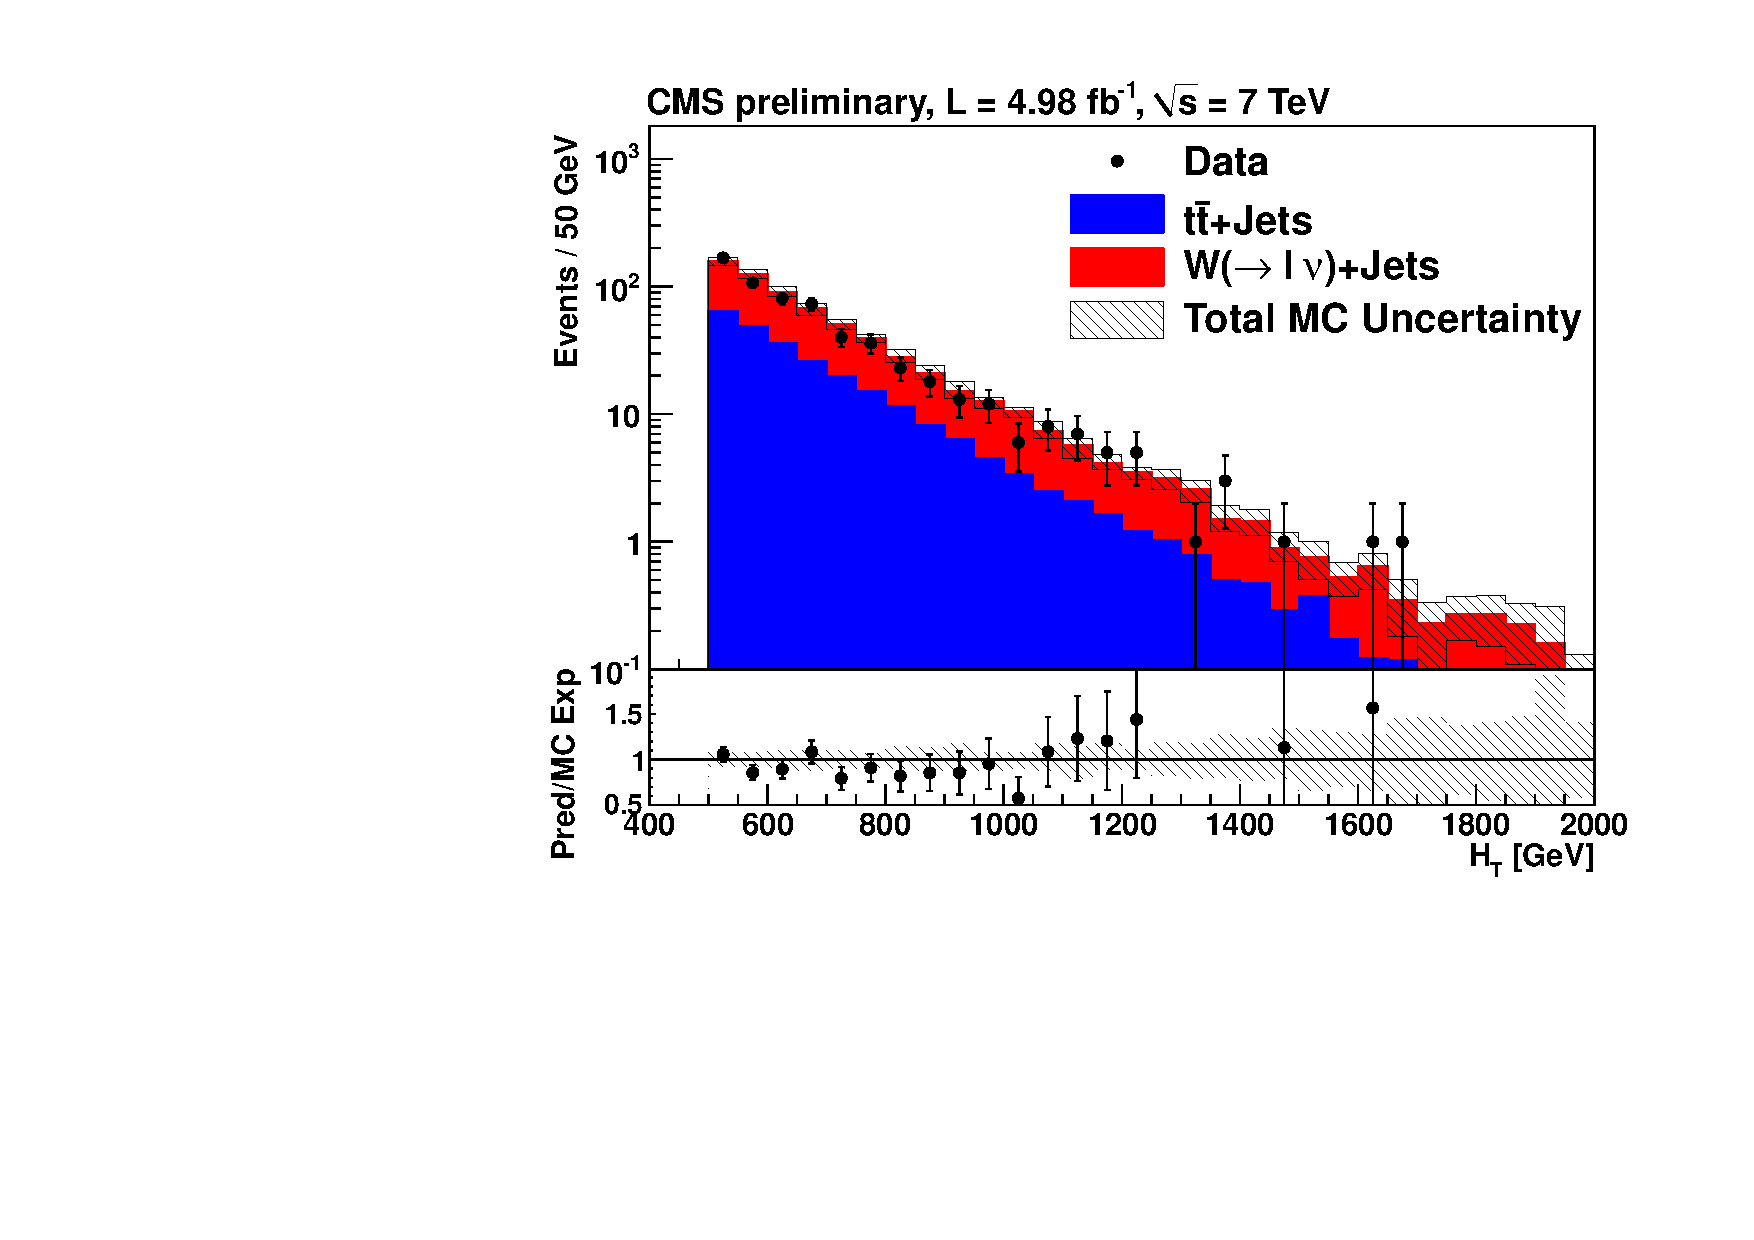
\includegraphics[width=0.9\textwidth]{lostlepton/plots/ANplots/Control_HT.pdf}\\
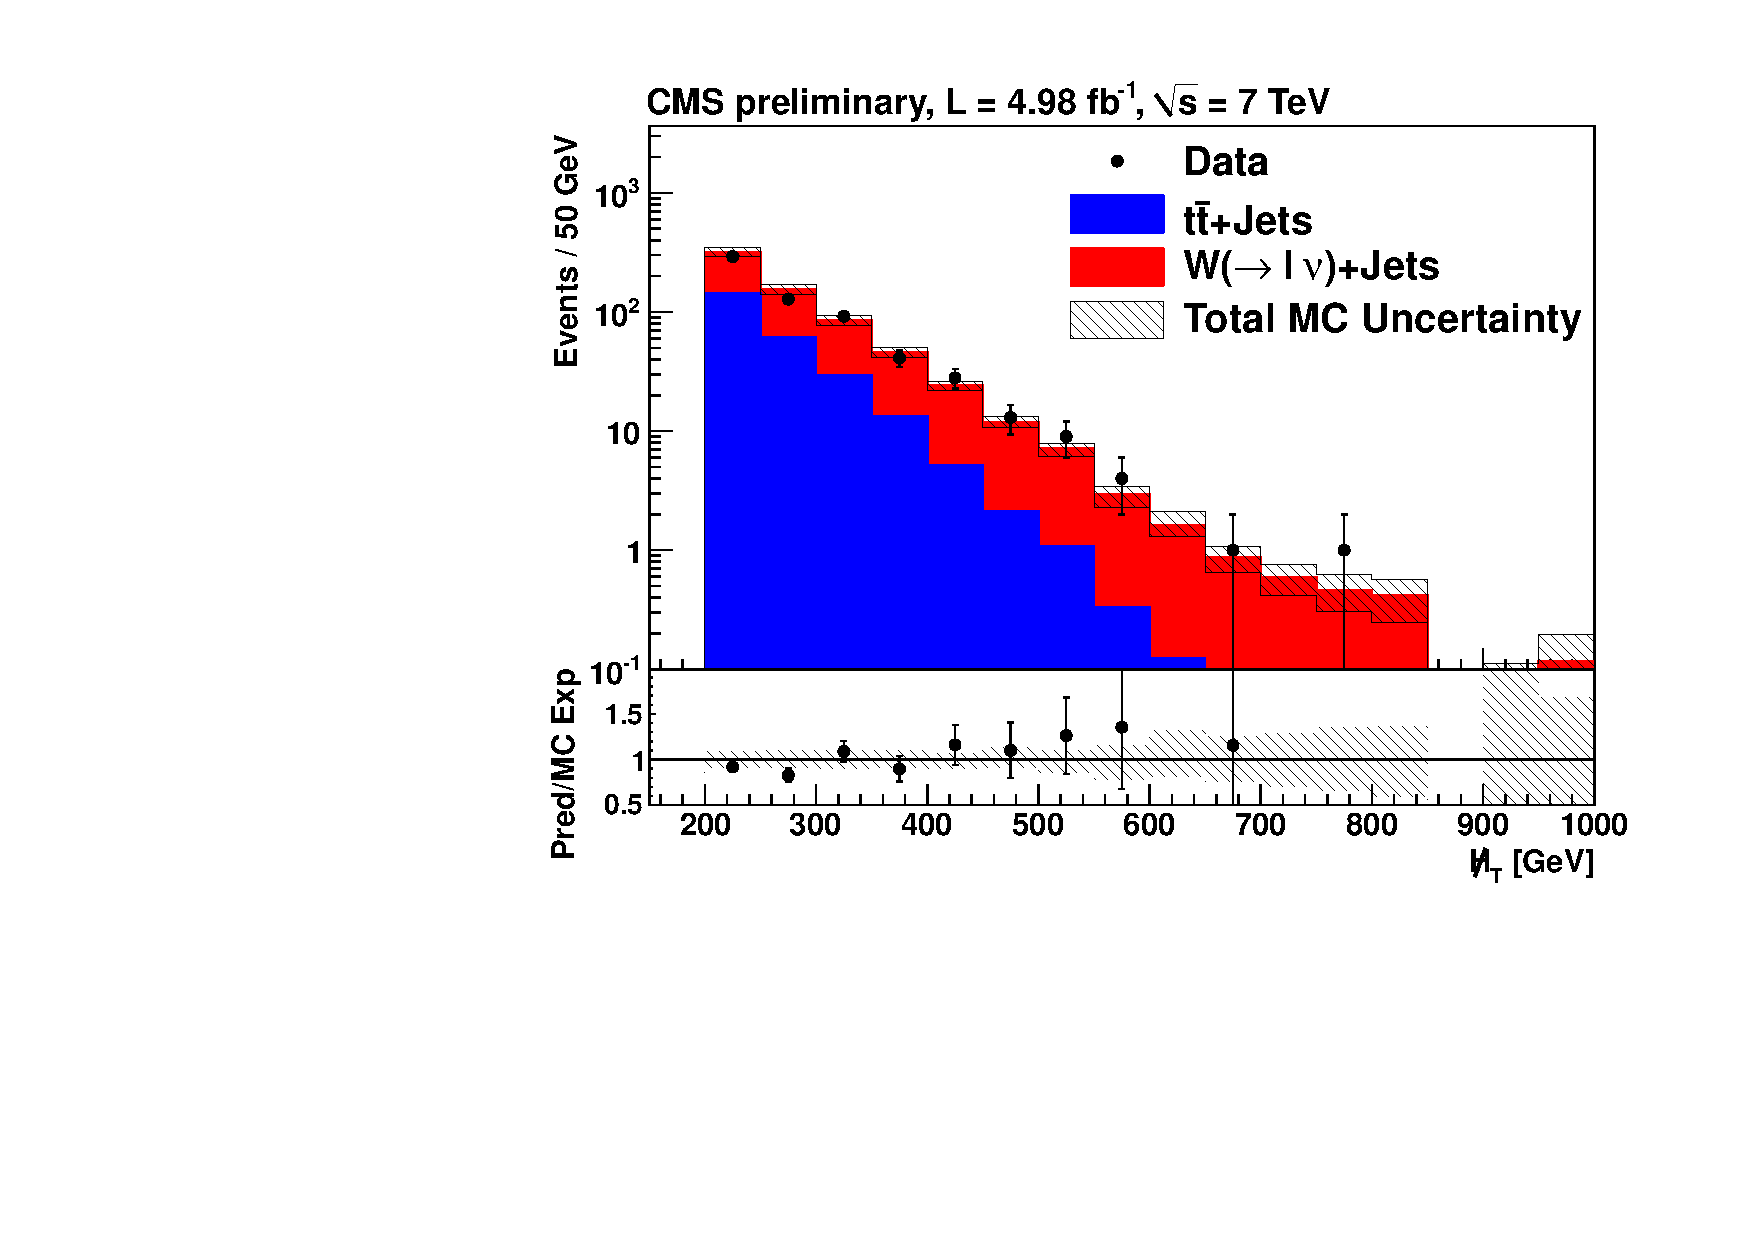
\includegraphics[width=0.9\textwidth]{lostlepton/plots/ANplots/Control_MHT.pdf}
%\includegraphics[angle=0,width=0.5\textwidth]{wtop_lostlepton_figures/MHTMHT_r}&
%\includegraphics[angle=0,width=0.5\textwidth]{wtop_lostlepton_figures/HTHT_r}
%%(a)&(b)\\
\end{tabular}
\end{center}
\caption{These figures show a comparison of the $\mu$ control sample for the \HT and \MHT distribution selected on data corresponding to the full \lumi recorded 2011 and simulated \ttbar and \wpj events.}

\end{figure}

% Data-MC comparison


\clearpage


\subsection{Signal Contamination}
\label{sec:signal_contamination}
Events involving physics beyond the standard model can contain jets, missing transverse momentum and leptons, in particular muons in the final state. Such events can enter the CS leading to an over estimation of the lost-lepton background. This is referred to as ''signal contamination'' of the CS.\\ 
For the SM background the muons in the CS are products of a \W decay while this is generally not expected for signal events. The topology of the \W decay can be used to distinguish between SM background and signal events.
The transverse-mass-distribution (\mt) has shown to be a useful value to remove possible signal contamination of the CS.\\

 \begin{equation}
 m_{T} = \sqrt{2 p_{T}(\mu) \met (1 - \cos(\Delta \Phi))}
\label{eq:mt}
\end{equation}
with $p_{T}(\mu)$ being the \pt of the muon in the CS, $\hspace{1mm} \met$ the missing energy in the event and $\Delta \Phi$ being the angel between the $\vec{\met}$ and the $\mu$.\\
\begin{figure}[tbhn]
\begin{center}
\begin{tabular}{c}
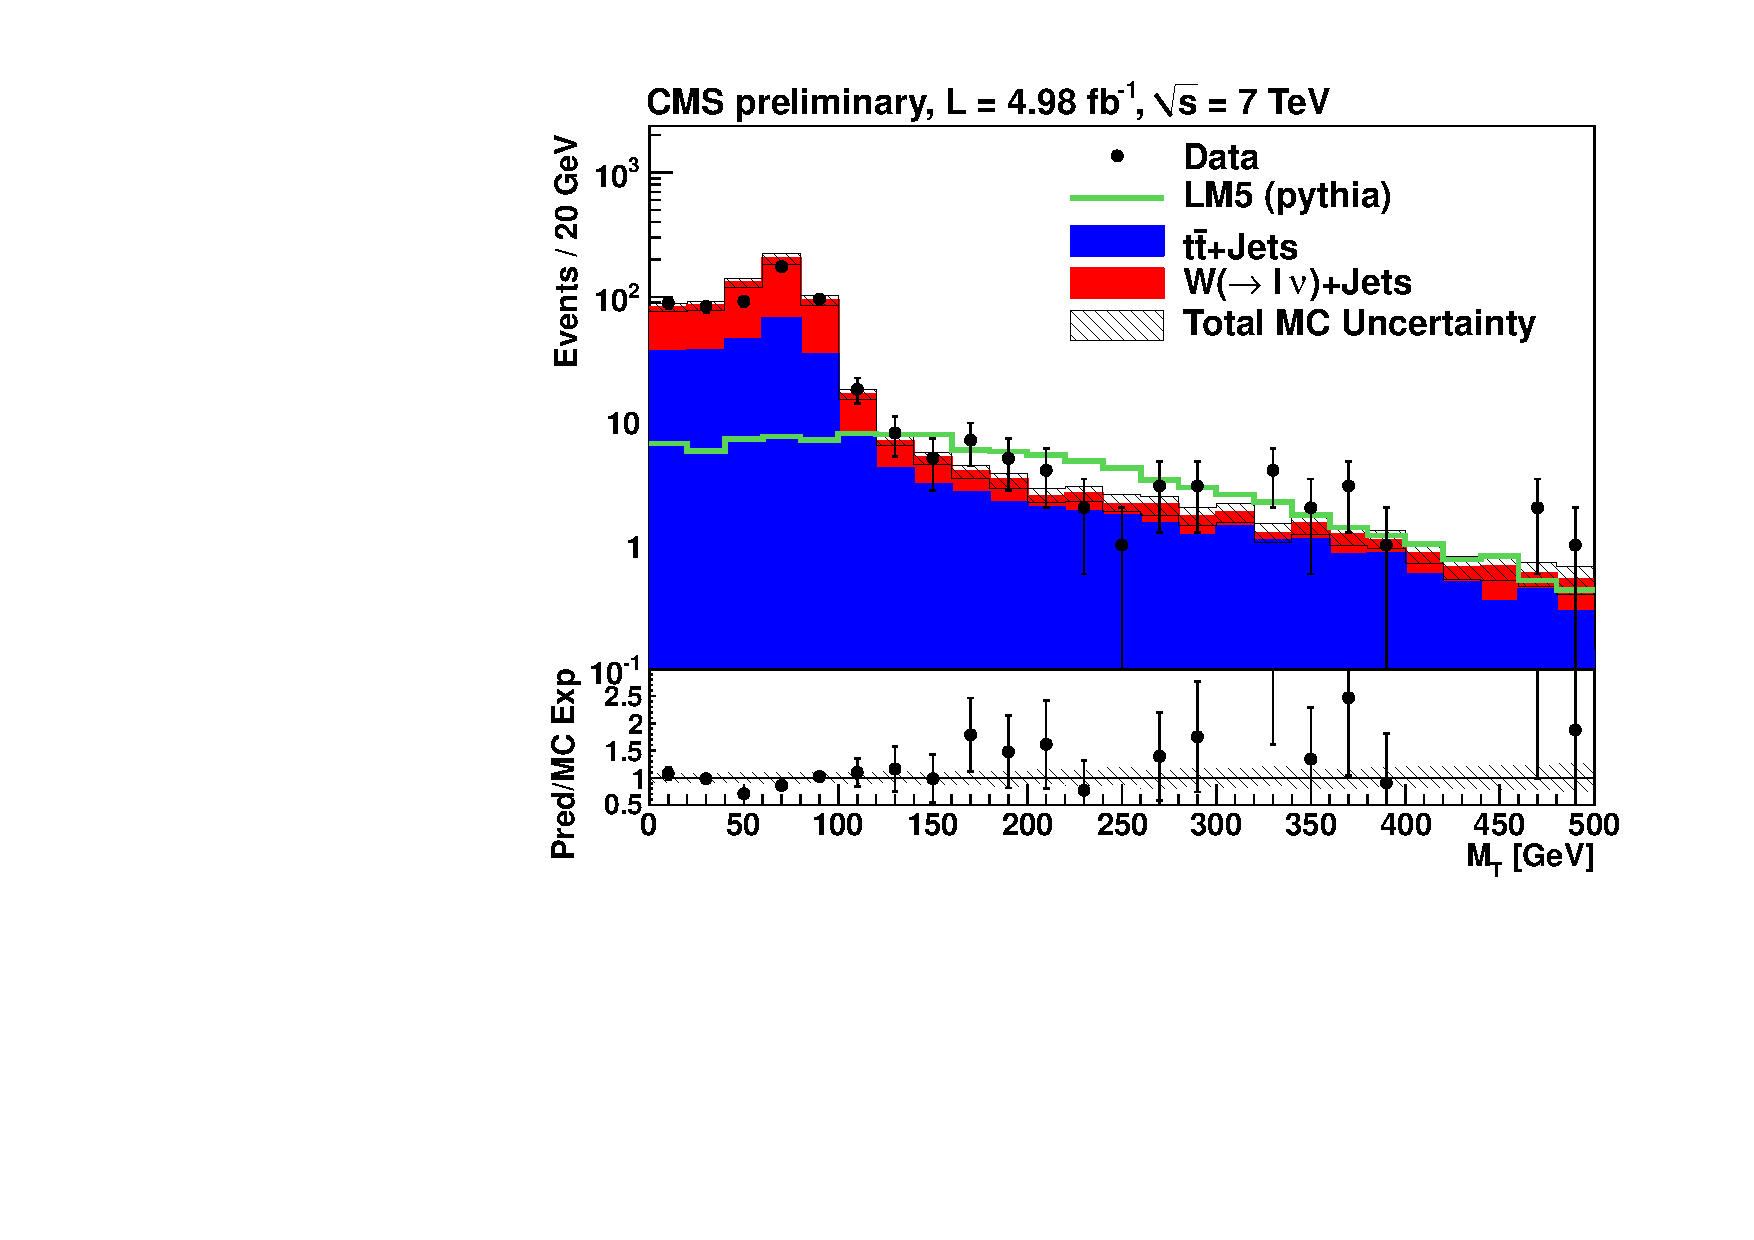
\includegraphics[width=1\textwidth]{lostlepton/plots/ANplots/Control_MTW.pdf}\\
\end{tabular}
\end{center}
\caption{This plot shows the \mt distribution of the control sample in data, for simulated \ttbar and \wpj events and for an example signal point (LM5). The \mt distribution of the CS steeply falls above $80 \gev$ for the SM process, where as the LM5 distribution is rather wide. (The legend description can be found in the caption of Fig.~\ref{fig:LostLepton_MuCS_data_MC})}
\label{fig:control_mtw}
\end{figure}
Fig.~\ref{fig:control_mtw} shows the \mt for the CS selected on data and MC together with the LM5 cMSSM benchmark point.
For the SM background events the transverse-mass-distribution rises up to the \w mass of 80.4 \gev above which it steeply falls while a broad distribution is being observed for signal events (LM5).\\
A cut at 100 \gev to remove everything above has shown a good balance between Standard Model CS reduction and signal contamination rejection. Note that because of the detectors finite resolution of muon and jet \pt some cases have a \mt value higher than $m_W$\footnote{Also the small amount of dileptonic \ttbar decays lead to higher \mt.}.\\
The efficiency, defined as the ratio of Standard Model CS events passing the cut to all Standard Model CS events, for the search regions and the baseline selection can be seen in Fig.~\ref{fig:mt_cut_eff}. The error bars cover the statistical uncertainty of the used MC. A good efficiency of about 90\% can be observed for all regions.\\
A constant correction factor of 10\% together with an uncertainty of 4.0\% is applied on data to correct for the removed Standard Model CS and cover for the variation of the cut efficiency.\\
Overall, possible signal contamination leading to an over estimation of the background and therefore a reduction of the sensitivity of the analysis to new particles has been reduced by the \mt cut, increasing the capability of the analysis of finding new physics.
\begin{figure}[tbhn]
\begin{center}
\begin{tabular}{c}
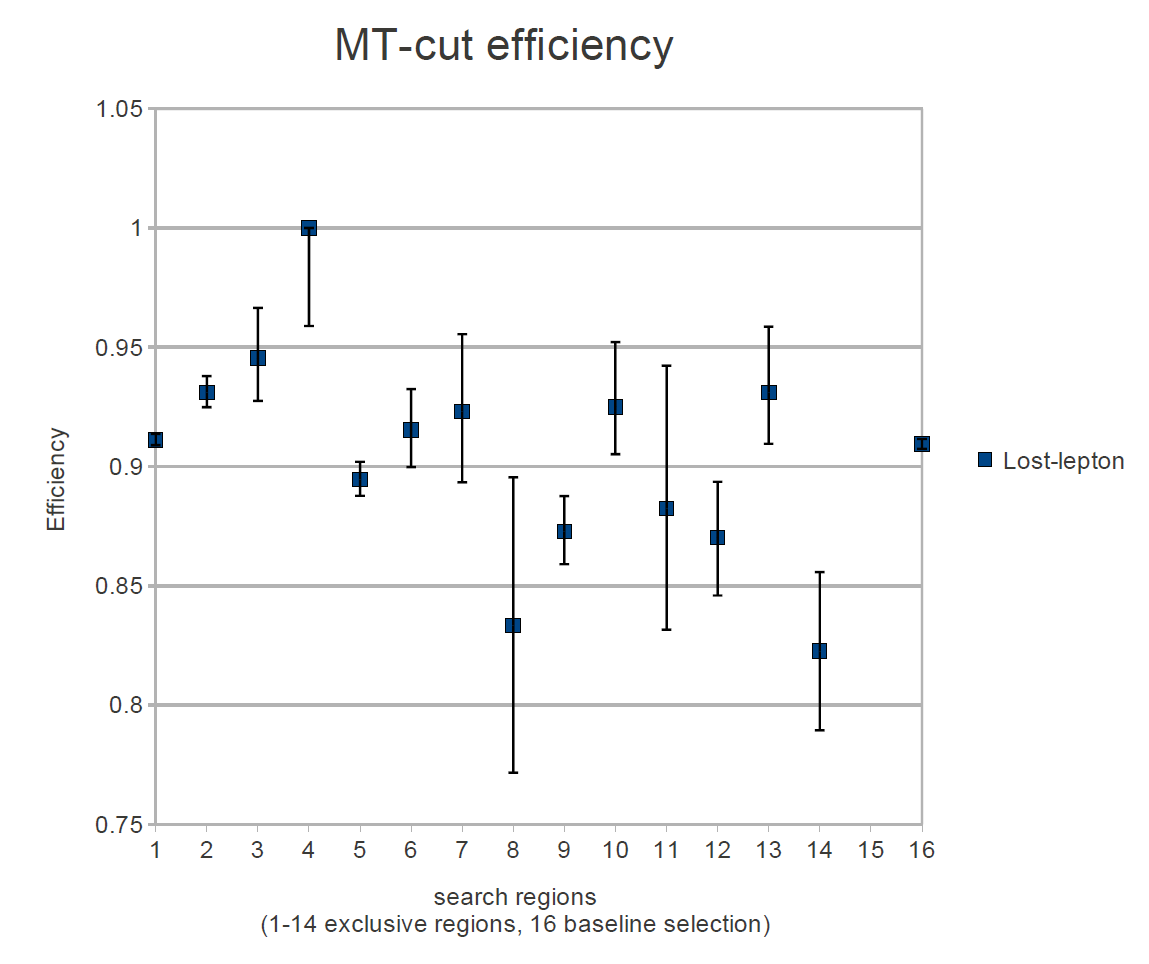
\includegraphics[width=1\textwidth]{lostlepton/plots/MT_eff.png}\\
\end{tabular}
\end{center}
\caption{This plot shows the efficiency of the $\mt$ cut for all exclusive regions (the numbering corresponds to the enumeration in Tab.\ref{tab:regions}) for bin 1-14. Bin 16 shows the value for the baseline selection. }
\label{fig:mt_cut_eff}
\end{figure}



% used in the selection by rejecting events with a reconstructed \W mass above 100 \gev. The removed CS amount which is above 100 \gev is being corrected for. Fig. \ref{fig:mt_LM5_baseline} shows the \mt distribution for the baseline selection of the CS and an example SUSY signal point.\\

%It is possible to calculate from the decay products, namely the muon and the $\met$ from the neutrino the transverse component of the \W mass. The muon is being reconstructed with its angel $\phi$, $\eta$ and \pt. The \met comes ideally from the not detected $\nu$. The combination of $\Delta \phi$ between the $\met$ and the muon together with the \pt of the muon and the $\met$ represents the ''transverse mass'' \mt of the decaying particle. 
% \begin{equation}
% m_{T} = \sqrt{2 p_{T}(\mu) \slash \met (1 - \cos(\Delta \Phi))}
%\label{eq:mt}
%\end{equation}
%The transverse-mass-distribution rises up to the \w mass of 80 \gev above which it steeply falls. Since the detector has a finite resolution of the muon \pt and jets are measured with an uncertainty on the energy \mt reconstructed higher than 80 \gev are expected. The cut is applied at 100 \gev to keep the reduction of the CS small. Studies have been done for different \HT and \MHT cuts on MC comparing the amount of muons passing and failing the \mt cut to evaluate the \mt cut correction factor. The resulting $\mt$ cut efficiencies can be seen in fig.\ref{fig:mt_cut_eff}. The error bars cover the statistics of the MC where positive error bars show Poisson errors while Gaussian error bars are used for the negative errors. A constant correction factor of 10\% for all regions is justified combined with the statistical uncertainty of the cut efficiencies and the assigned uncertainty of 43\% on the cut.\\
%Outliers are coming from mis-measurements of the muon \pt and the jets or from dileptonic \ttbar decays. These fraction of the CS is being removed by the $\mt$ cut. .\\
%For events where the $\met$ is caused by, for example, a LSP the cut becomes more efficient for higher \HT and \MHT selections since the \mt coming from LSPs is broadly distributed, as can be seen for the baseline selection in fig. \ref{fig:mt_LM5_baseline}.\\



 






\subsection{Other SM background contributions}
\label{sec:other_sm_contribution}
The main SM background contributing to lost-lepton CS arises as discussed from \ttbar and \wpj events. However other processes can contribute by ending up in the CS. There are QCD events, $ZZ$ or $Z$  processes which can have the same signature and contribute to the background.\\
The samples listed in Tab.~\ref{tab:MC_samples} have been used to study these backgrounds by selecting a control sample on the corresponding MC samples.
Tab.~\ref{tab:other_sm_contribution} shows the amount of events for each of the other SM backgrounds scaled to the full luminosity of \lumi. No considerable amount of events has been found. An uncertainty of less than $3\%$ is justified to cover for these SM background contributions and for possible other contributions which are expected to be magnitudes below the listed ones.

\begin{table}[htb]
\begin{center}
    \begin{tabular}{|l|l|l|l|}
        \hline
			& Number of Events in the CS 	& $\pm$         & ratio[\%]	\\  \hline
        $QCD$ 		&0 				& 0 		&0		\\ 
        $ZZ$   		&0.04  				& 0.02		&0.0	 	\\
        $Z$    		&7.99  				& 2.02		&1.2 		\\ 
        $Summe$ 	&8.03				& 2.04		&1.2 		\\ \hline
	\wpj \& \ttbar 	& 658.20	&5.00  & 100   \\ 
%        \ttbar &  --	   & ---     \\
        \hline

    \end{tabular}
\caption{This table shows the amount of additional SM processes which add to the CS selected on MC compared to the selection from \ttbar and \wpj events. The shown ratio is defined as SM background divided by the main background (\ttbar and \wpj). All numbers are scaled to the full luminosity of \lumi .\label{tab:other_sm_contribution}}
\end{center}


\end{table}

\clearpage






\section{Predicting the lost electrons and muons}
\label{sec:ll_prediction}
% sketch of the control sample
\begin{figure}[tbhn]
\begin{center}
\begin{tabular}{c}
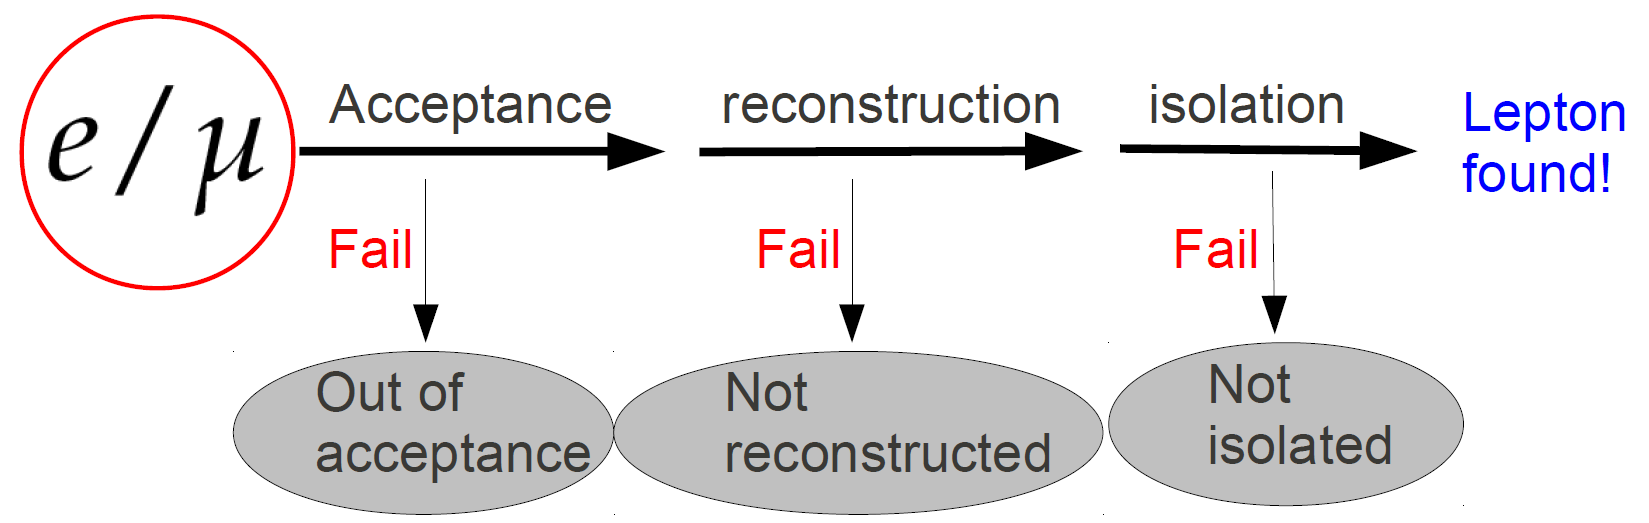
\includegraphics[width=0.80\textwidth]{lostlepton/plots/lepton_veto_sketch.png}\\
\end{tabular}
\end{center}
\caption{Visualization of the steps a muon has to take in order to enter the control sample}
\label{fig:sketch_lepton_veto}
\end{figure}
There are three steps a lepton has to take to be rejected by the lepton veto.
\begin{enumerate}

 \item First it has to be within the detector acceptance. 
 \item The second step is the reconstruction. 
 \item The final step is the isolation criteria.
\end{enumerate}
The CS is weighted according to each efficiency individually. 
Fig.~\ref{fig:sketch_lepton_veto} shows a chart of this three steps.\\
Since the control sample of well identified and isolated muons is used, one has to start predicting the three steps in reversed order.\\
Starting with modeling the not isolated muons followed by predicting the not reconstructed and finally the out of acceptance muons.
To model the not isolated muons the CS is weighted according to:
\begin{equation}
 \rm !ISO^{\mu} = {\rm CS}\cdot \frac{1-\epsilon_{\rm ISO}^{\mu}}{\epsilon_{\rm ISO}^{\mu}} 
    %%   \rm !ISO^{\mu}} = {\rm CS}\cdot \frac{1-\epsilon_{\rm ISO}^{\mu}}{\epsilon_{\rm ISO}^{\mu}} 
\label{eq:isolation_muon}
\end{equation}
with $\rm !ISO^{lepton}$ being the applied weight and $\epsilon_{X}^{\mu/e}$ being the efficiency of the criteria $X$ for the lepton.\\
The next step is to model the not reconstructed muons which is done by taking the muon isolation and reconstruction (in)efficiency into account. The weight is calculated according to the following equation:
\begin{equation}
 {\rm !Reco^{\mu}} = {\rm CS}\cdot \frac{1}{\epsilon_{\rm ISO}^{\mu}} \cdot \frac{1-\epsilon_{\rm Reco}^{\mu}}{\epsilon_{\rm Reco}^{\mu}}
\label{eq:reconstruction_muon}
\end{equation}
The last step in modeling the lost muons is to take also the muons into account which fall out of the detector acceptance. The weight has to include the isolation and reconstruction (in)efficiencies together with the out of acceptance efficiency:
\begin{equation}
 {\rm !Acc^{\mu}} = {\rm CS}\cdot \frac{1}{\epsilon_{\rm ISO}^{\mu}}\cdot \frac{1}{\epsilon_{\rm Reco}^{\mu}} \cdot \frac{1-\epsilon^{\mu}_{Acc}}{\epsilon^{\mu}_{Acc}}
\label{eq:acceptance_muon}
\end{equation}
The electrons are modeled using the same muon CS. This is valid since the decay of a $W$ to a $\mu$ or $e$ has according to the lepton universality the same probability\cite{bib:berger}.
All muon (in)efficiencies need to be taken into account before modeling the lost electrons resulting in more complex equations. The following equations are used to model the not isolated (Eq.~\ref{eq:elec_iso}), not reconstructed (Eq.~\ref{eq:elec_reco}) and the out of acceptance electrons (Eq.~\ref{eq:elec_acc}). 
\begin{equation}
{\rm !ISO^{e}} = {\rm CS}\cdot \frac{1-\epsilon_{\rm ISO}^{e}}{\epsilon_{\rm ISO}^{\mu}} \cdot \frac{\epsilon^{e}_{Reco}}{\epsilon^{\mu}_{Reco}} \cdot \frac{\epsilon^{e}_{Acc}}{\epsilon^{\mu}_{Acc}}
\label{eq:elec_iso}
\end{equation}
\begin{equation}
{\rm !Reco^{e}} = {\rm CS}\cdot \frac{1}{\epsilon_{\rm ISO}^{\mu}}\cdot \frac{1-\epsilon_{\rm Reco}^{e}}{\epsilon_{\rm Reco}^{\mu}}  \cdot \frac{\epsilon^{e}_{Acc}}{\epsilon^{\mu}_{Acc}}.
 \label{eq:elec_reco}
\end{equation}
\begin{equation}
{\rm !Acc^{e}} = {\rm CS}\cdot \frac{1}{\epsilon_{\rm ISO}^{\mu}}\cdot \frac{1}{\epsilon_{\rm Reco}^{\mu}}  \cdot \frac{1 - \epsilon^{e}_{Acc}}{\epsilon^{\mu}_{Acc}}
 \label{eq:elec_acc}
\end{equation}

%\begin{equation}
%{\rm !ID^{e}} = {\rm CS}\cdot \frac{1}{\epsilon_{\rm ISO}^{\mu}}\cdot \frac{1-\epsilon_{\rm ID}^{e}{\epsilon_{\rm ID}^{\mu}}  \cdot \frac{\epsilon^{e}_{Acc}}{\epsilon^{\mu}_{Acc}}.
% \label{eq:elec_acc}
%\end{equation}
The final equation to predict all lost leptons is:
\begin{equation}
\label{eq:totalWeight}
 \text{all lost leptons} = C \cdot \sum_{i=e,\mu}\left(\text{!Iso}^i+\text{!Reco}^i+\text{!Acc}^i\right) 
\end{equation}
with $C$ being a correction factor consisting of the correction factor for the \mt cut efficiency discussed in Sec.~\ref{sec:signal_contamination}, a small factor for di-leptonic events discussed in Sec.~\ref{sec:controlSample} and a ''non-closure'' factor discussed in Sec.~\ref{sec:closure_test}.





\clearpage

\section{Lepton Efficiencies}
\label{sec:efficiencies}
This chapter describes how the six efficiencies, used to weighted the CS, are obtained.\\
The acceptance efficiency has been calculated from MC by comparing the amount of leptons fulfilling the acceptance criteria defined in Sec.~\ref{sec:acceptance} to all prompt leptons. This has been done for the baseline selection without the lepton veto for muons and electrons separately.\\
The isolation efficiencies, taken from \cite{bib:phd:jan}, were obtained by a Tag\&Probe method (Sec.~\ref{sec:tag_probe}) on the Z-Resonance. The efficiencies are parametrized in $\frac{p_{t,lep}}{p_{t,jet}}$, with $p_{t,lep}$ being the lepton and $p_{t,jet}$ being the \pt of the closest jet, and $\Delta R$ to the closest jet. \\
This is necessary since the lepton isolation depends strongly on the activity around the lepton (see Sec.~\ref{sec:event_selection}) and the selection of the $Z$-Resonance has a different topology than the topology of the signal.\\
The reconstruction efficiencies are obtained from MC by calculating the ratio of generator leptons which can be matched to reconstructed leptons.\\ %Other parametrization of the reconstruction efficiencies have been test including Tag\&Probe reconstruction efficiencies in $\eta$ and lepton \pt but they fail in accounting for the topological differences. Therefore the reconstruction efficiencies have to be obtained from MC. 
\subsection{Tag\&Probe method}
\label{sec:tag_probe}
Tag\&Probe methods are well established methods to measure the efficiency of detectors to identify and isolate leptons. The idea is to take a well known process which has a good understood final state of two leptons and good understood background processes (a fit function is used to model the background from other processes).\\
For the here presented efficiencies the $Z$-resonance was used. 
The $Z$-boson can only decay to two leptons, two jets or two neutrinos. Therefore if one lepton is found another lepton of the same flavor must be in the event too.\\
The Tag\&Probe method starts with a well identified ''tag''-lepton. The tag-lepton has to pass tight identification cuts to make sure that it is a proper prompt lepton.\\
To leave other possible leptons in the event unbiased this tag-leptons are required to fire the trigger used for the sample selection.\\
Then another lepton (''probe''-lepton) in the event is selected without any isolation and, depending on the to be probed efficiency, suitable reconstruction criteria. When this lepton is found both are combined to the mass of the $Z$-Boson. Only events with a reconstructed mass between 60 and 120 \gev for muons and 70 to  110 \gev for electrons are used.\\
Then the isolation criteria or reconstruction criteria are applied to the probe-lepton, resulting in a fraction of probe-leptons passing and failing the isolation criteria. A function to each fraction is fitted modeling the $Z$-resonance together with the other (exponentially decreasing) background events. The ratio of the integral of both signal fits are used as isolation efficiency. The fitting uncertainty is included in the efficiency as uncertainty (more details can be found here \cite{bib:phd:jan}). 




\subsection{Leptons out of the detector acceptance}
\label{sec:acceptance}
The out of detector acceptance leptons are defined as leptons with $\pt<10GeV$ and muons with a $|\eta|>2.4$ (electrons $|\eta|>2.5$) which can not be detected (see Sec.~\ref{sec:detector}). %In general the leptons coming from $\tau$ decays tend to have less \pt therefore are more often out of acceptance. 
For the high $\HT>500 \gev$ and $\MHT>200 \gev$ cuts the amount of leptons out of acceptance show no dependency on \HT or \MHT. For muons an acceptance efficiency of 84\% and for electrons 81\% has been found\footnote{The \HT and \MHT distribution for the out of acceptance leptons can be found in  Fig.\ref{fig:reco_acc_combined}.}. 

% This has been studied on MC and can be seen in \ref{fig:out_acceptance}.

%\begin{figure}[htbp]
%\begin{center}
%\begin{tabular}{cc}
%
\includegraphics[width=0.49\textwidth]{lostlepton/plots/FixMe.png}
%
\includegraphics[width=0.49\textwidth]{lostlepton/plots/FixMe.png}\\%%
%
%\end{tabular}
%\end{center}
%\caption{This figure shows the closure for muons out of acceptance in \HT and \MHT for \ttbar and \wpj combined. No trend for ether \HT nor \MHT can be observed.}
%\label{fig:out_acceptance}
%\end{figure}


%FIXME out of acceptance plot for HT MHT and Number of vertices.

\subsection{Not reconstructed leptons}
\label{sec:reconstruc}
For the reconstruction efficiencies of the electrons the Tag\&Probe method can not be used because the super clusters need to be cleaned by removing jets to have a significant purity of real electrons in the selection\cite{bib:phd:jan}.\\
In order to still use the same parametrization as for the isolation efficiencies the reconstruction efficiencies are obtained from MC. A conservative estimate of 9\% uncertainty is applied on the total prediction. In principle the $\mu$ could be calculated with the Tag\&Probe method.\\
Previously\cite{bib:phd:jan} the reconstruction efficiencies had been done with a Tag\&Probe method on data on the $Z$-Resonance with the parametrization of the efficiencies in $\frac{p_{t,lep}}{p_{t,jet}}$ and $\eta$. The prediction with the old efficiencies show a clear systematic under-prediction which is caused by the deficiency of the $\eta$ parametrization to account for the kinematic differences between the $Z$-Boson resonance and the search regions. \\ 
As explained above (see Sec.~\ref{sec:efficiencies}) it is not possible to use a parametrization as a function of $\Delta R$ to the closest jet in the Tag\&Probe method for the electrons, forcing the use of MC.\\
Fig.~\ref{fig:oldReco} shows a comparison of the closure tests for the prediction with the old efficiencies (right) and the new  prediction (left). A clear under-prediction can be observed for the old efficiencies while the new efficiencies show a very good closure.\\
Fig.~\ref{fig:reco_eff} shows the used electron and $\mu$ reconstruction efficiencies.

% old reco
\begin{figure}[tbhn]
\begin{center}
\begin{tabular}{c}
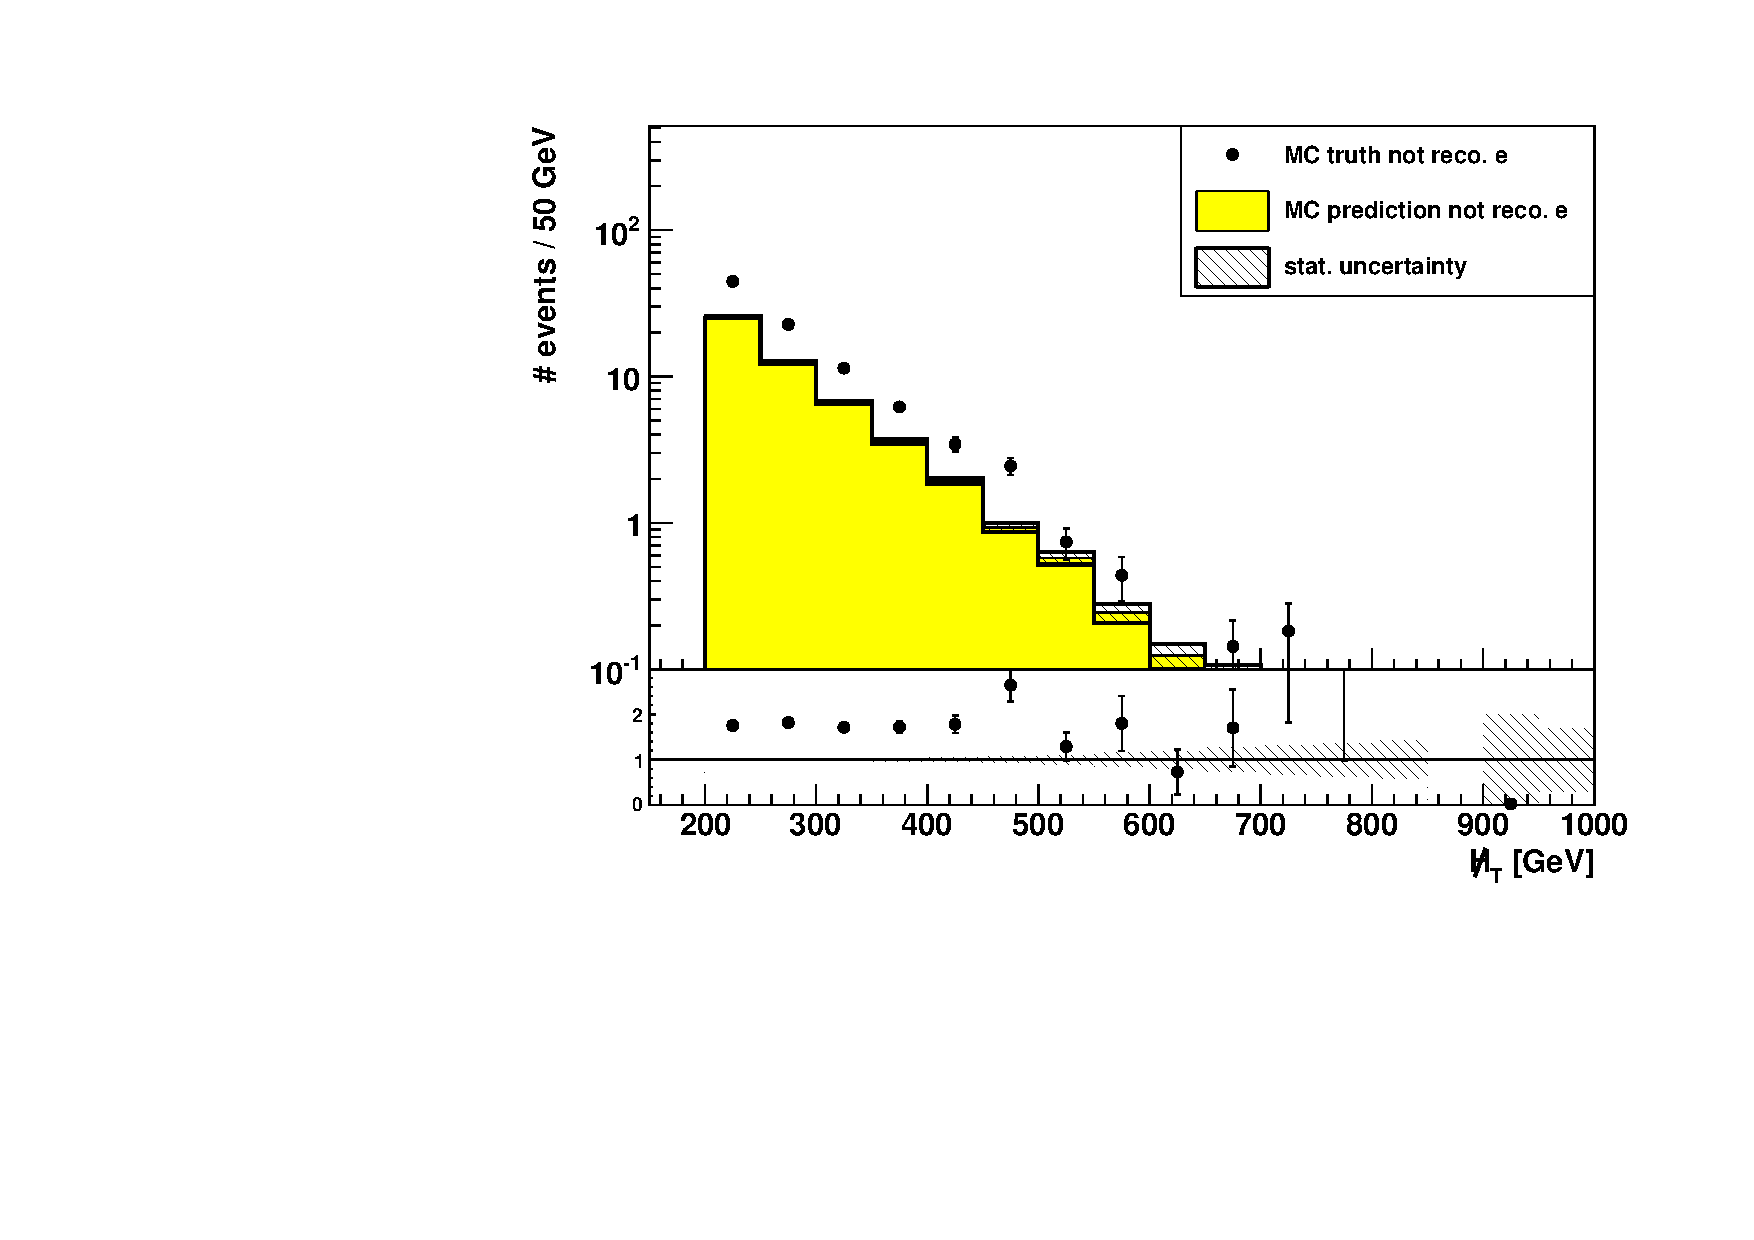
\includegraphics[width=.55\textwidth]{lostlepton/plots/MHTOldRecoE.pdf}
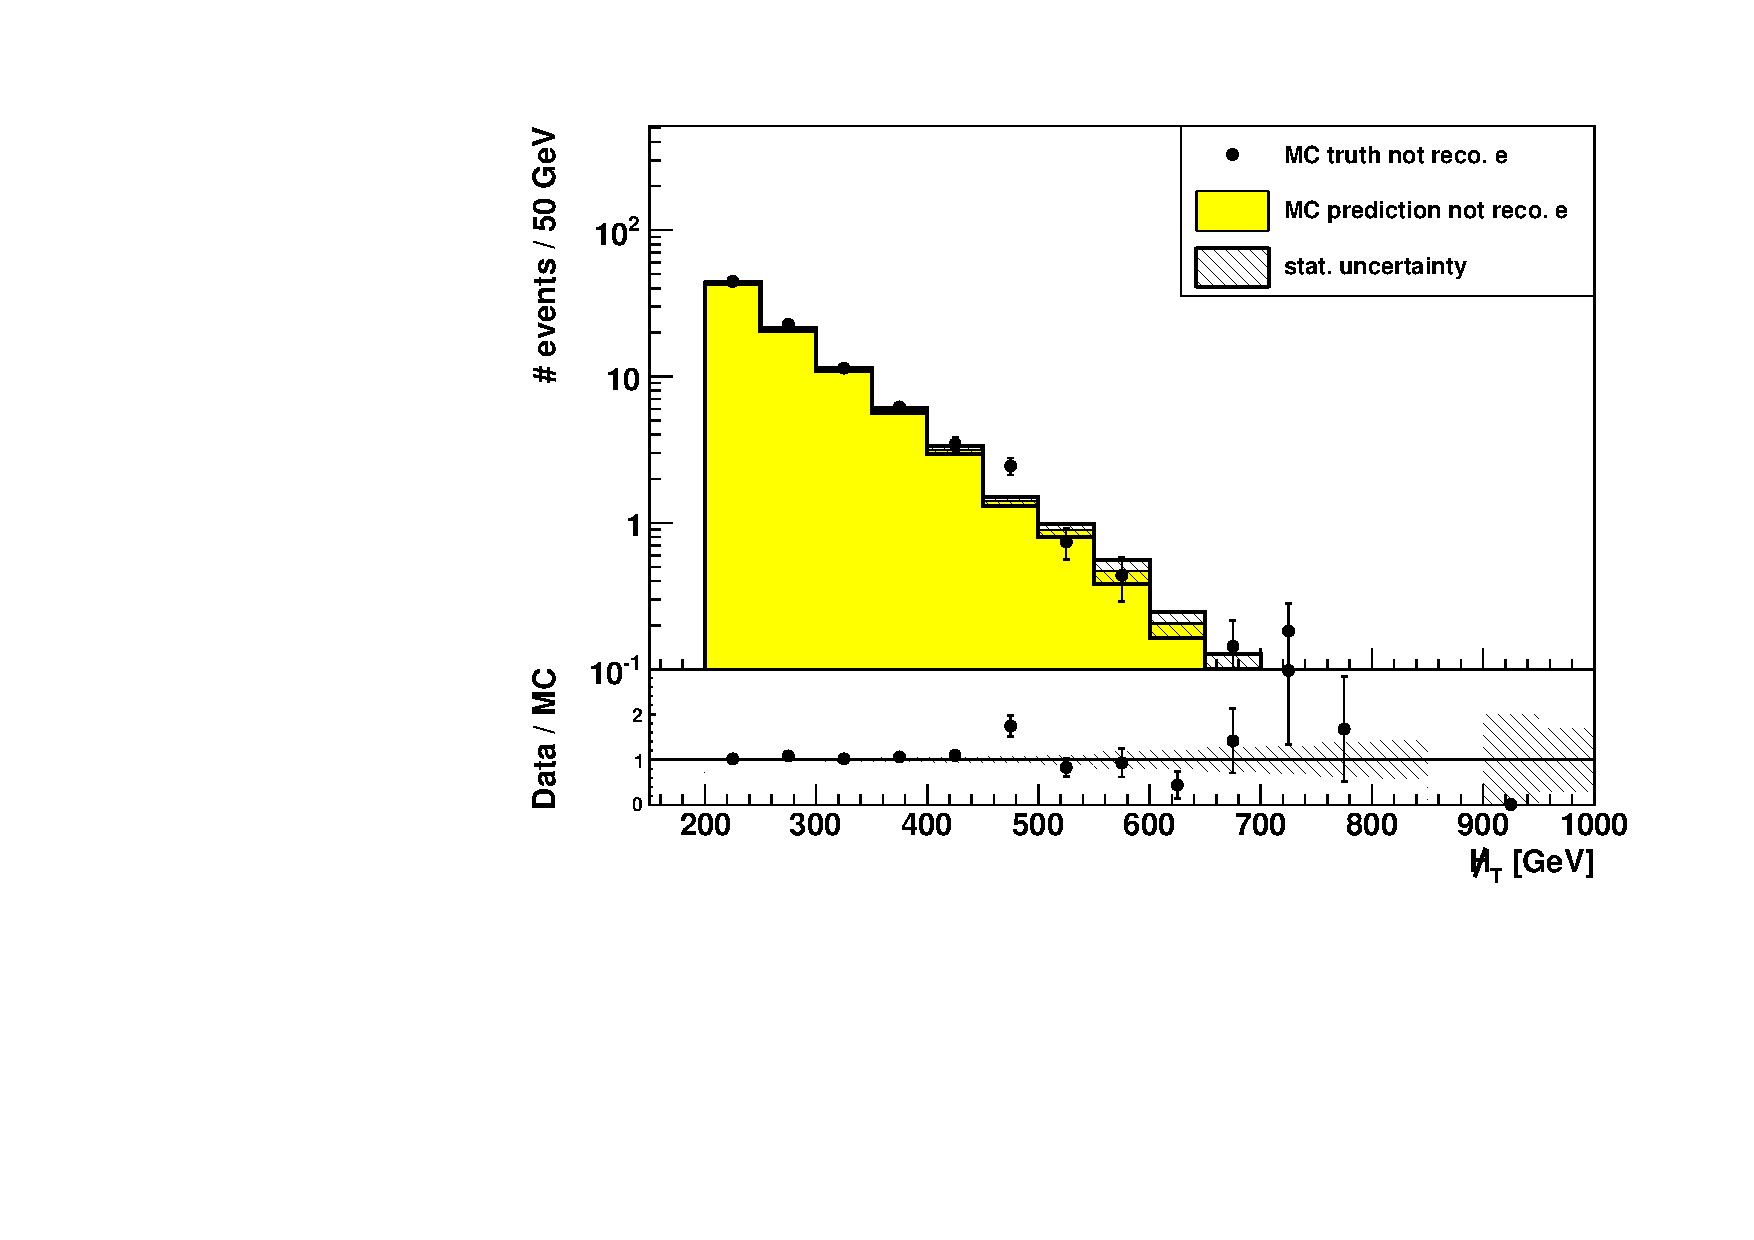
\includegraphics[width=.55\textwidth]{lostlepton/plots/MHTNewRecoE.pdf}\\
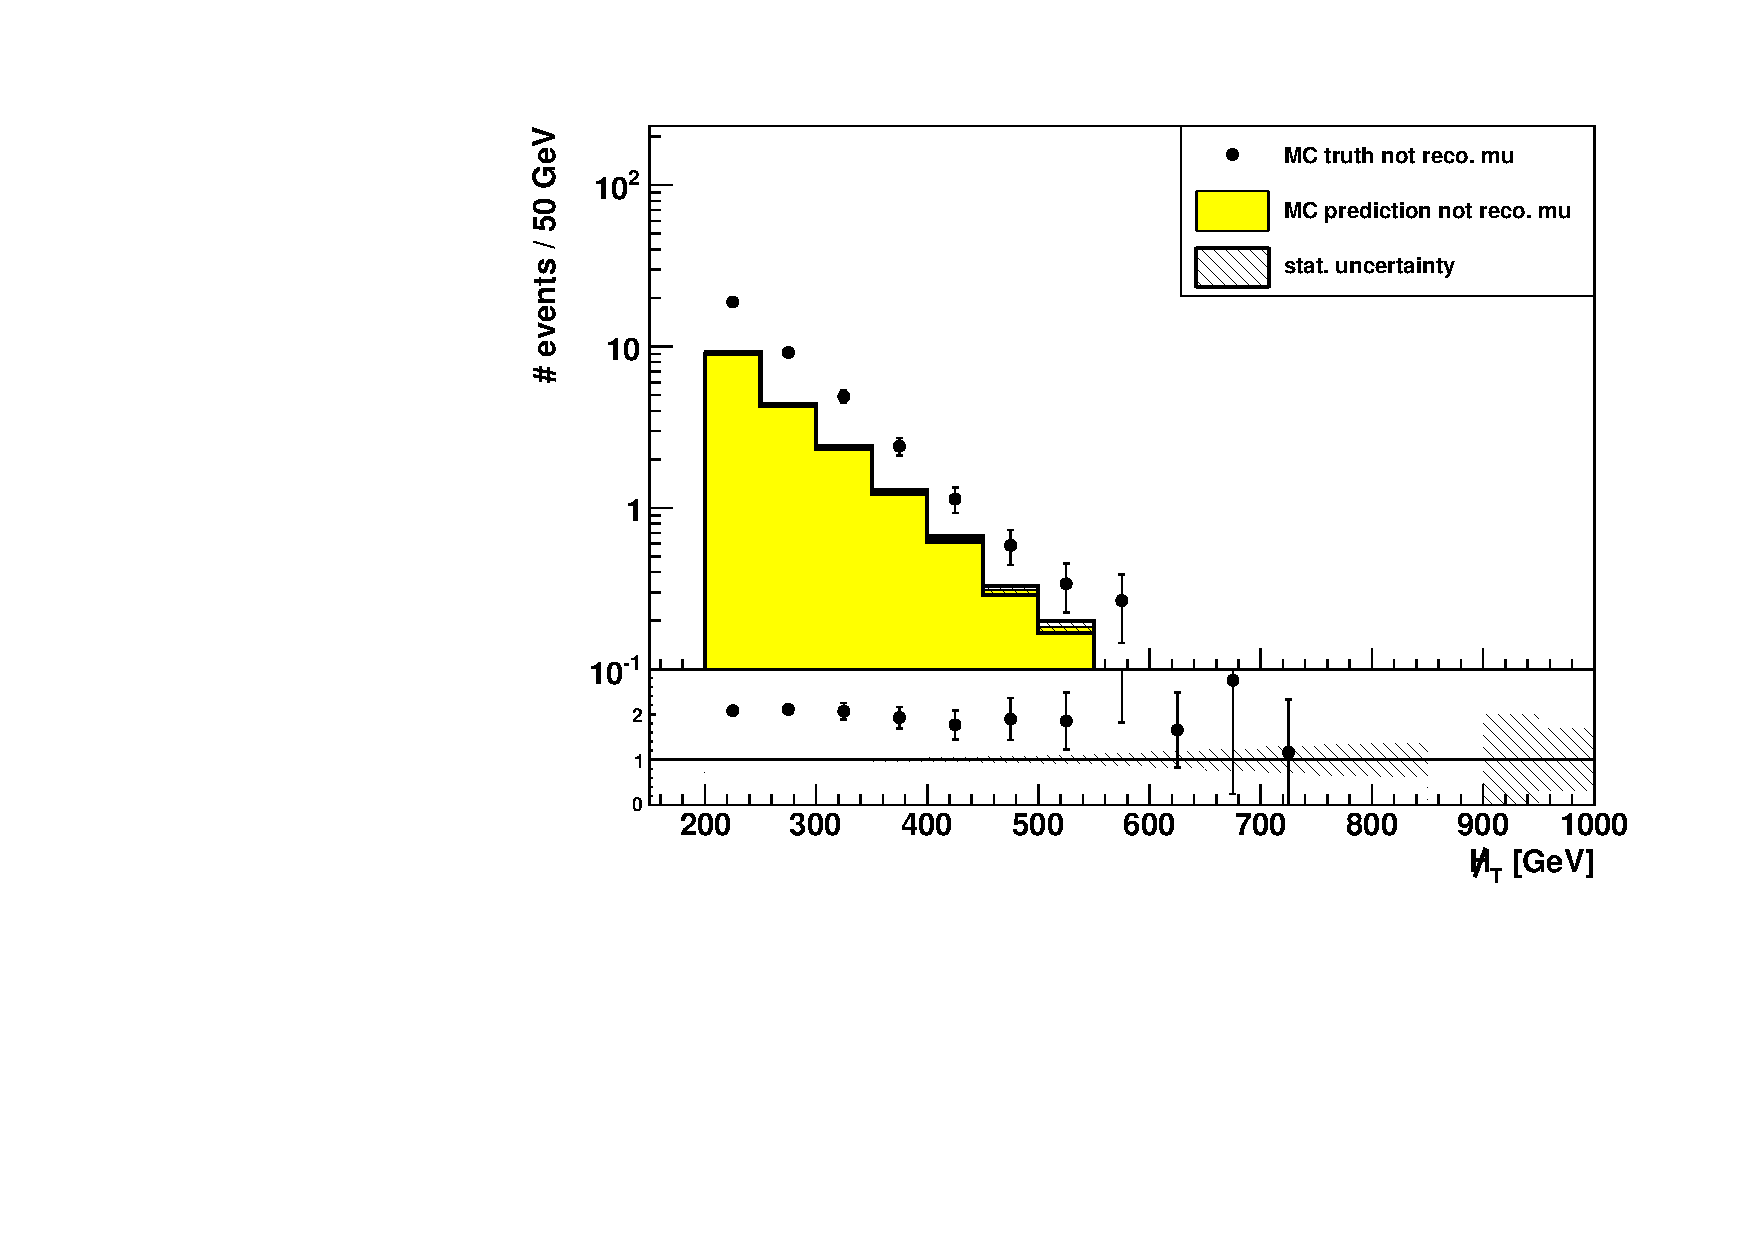
\includegraphics[width=.55\textwidth]{lostlepton/plots/MHTOldRecoMu.pdf}
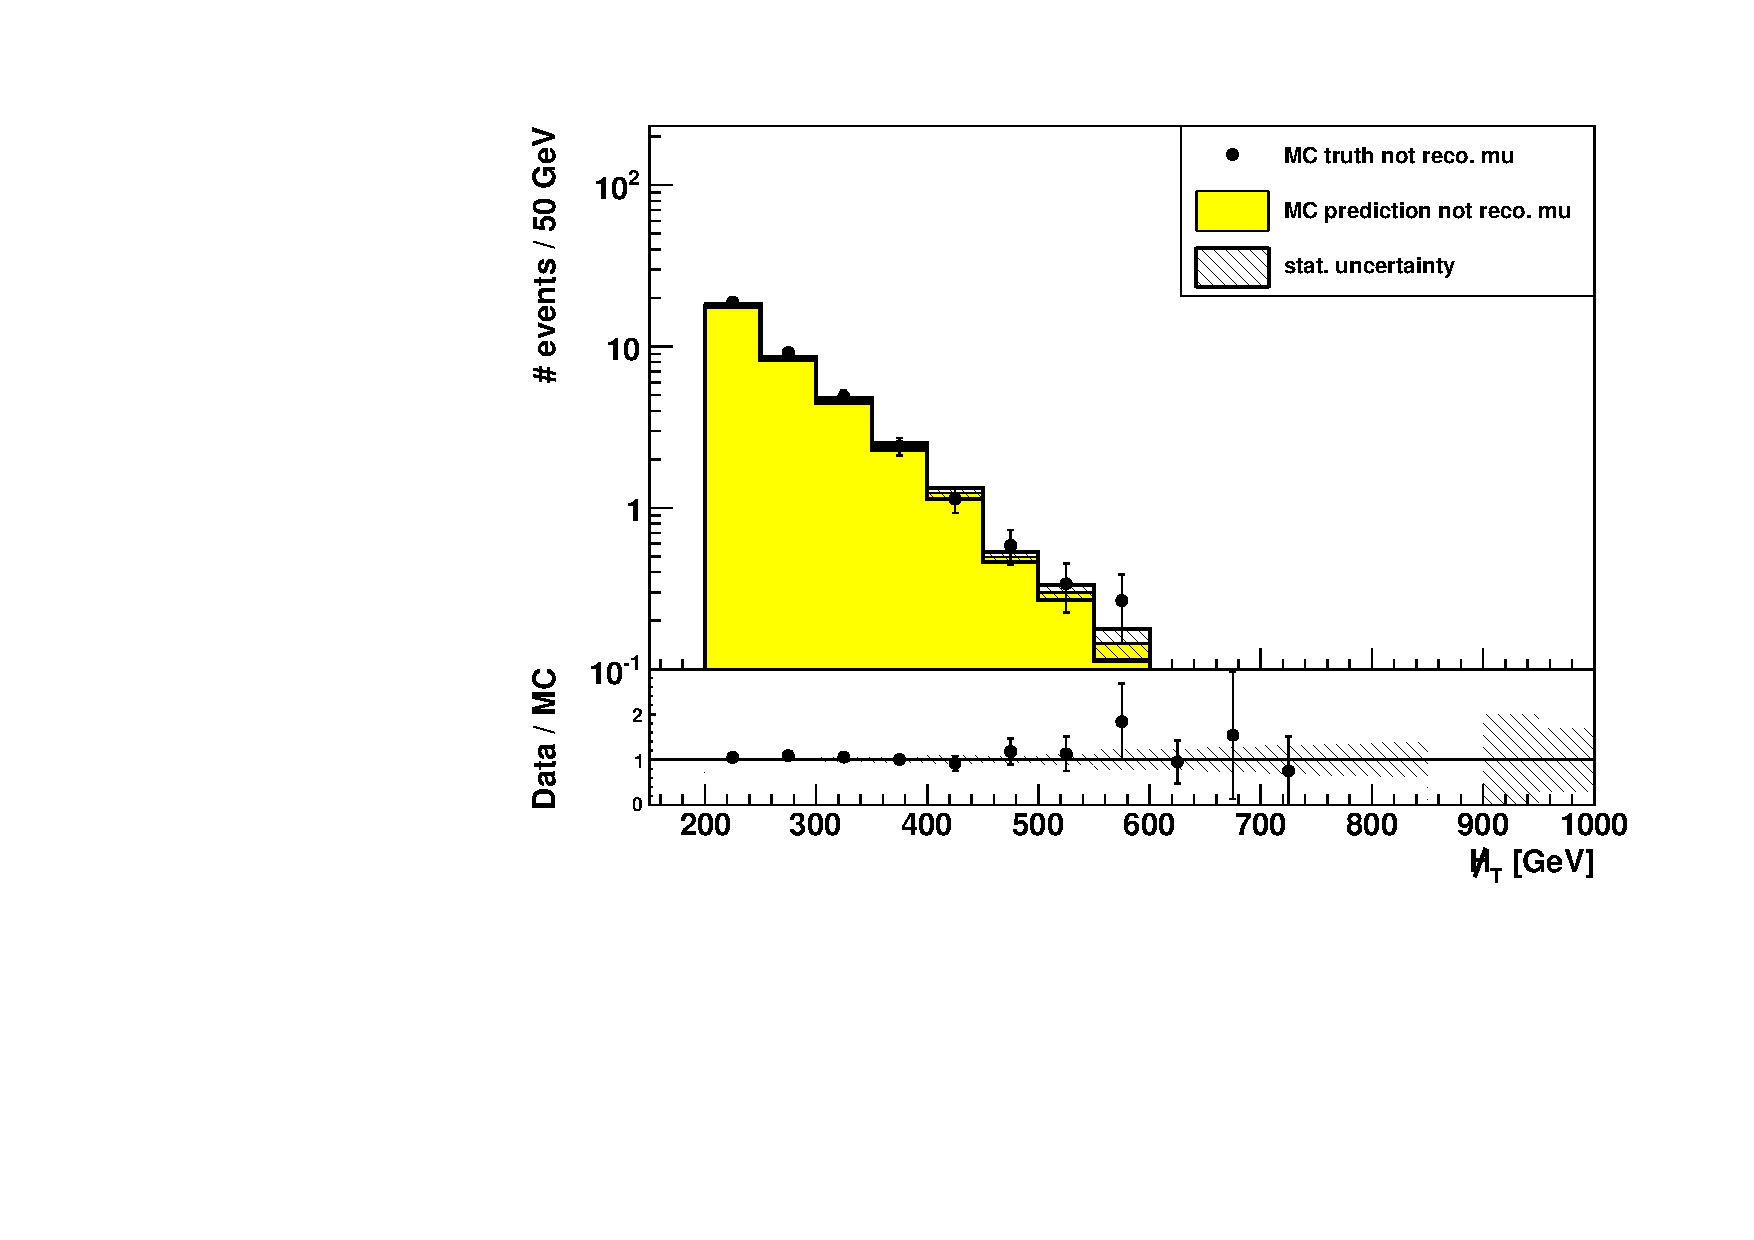
\includegraphics[width=.55\textwidth]{lostlepton/plots/MHTNewRecoMu.pdf}\\
%\includegraphics[angle=0,width=0.5\textwidth]{wtop_lostlepton_figures/MHTMHT_r}&
%\includegraphics[angle=0,width=0.5\textwidth]{wtop_lostlepton_figures/HTHT_r}
%%(a)&(b)\\
\end{tabular}
\end{center}
\caption{These plots show the MC closure (\ttbar and \wpj combined) for not reconstructed electrons (upper two plots) and muons (lower two plots). On the left side for the old efficiencies binned in $\frac{p_{t,lep}}{p_{t,jet}}$ and $\eta$ and on the right side with the new in lepton \pt and $\Delta R$ binned efficiencies.}
\label{fig:oldReco}
\end{figure}



%%% add 4 figures for not reco mu e ttbar and w separated
% iso eff
\begin{figure}[tbhn]
\begin{center}
\begin{tabular}{c}
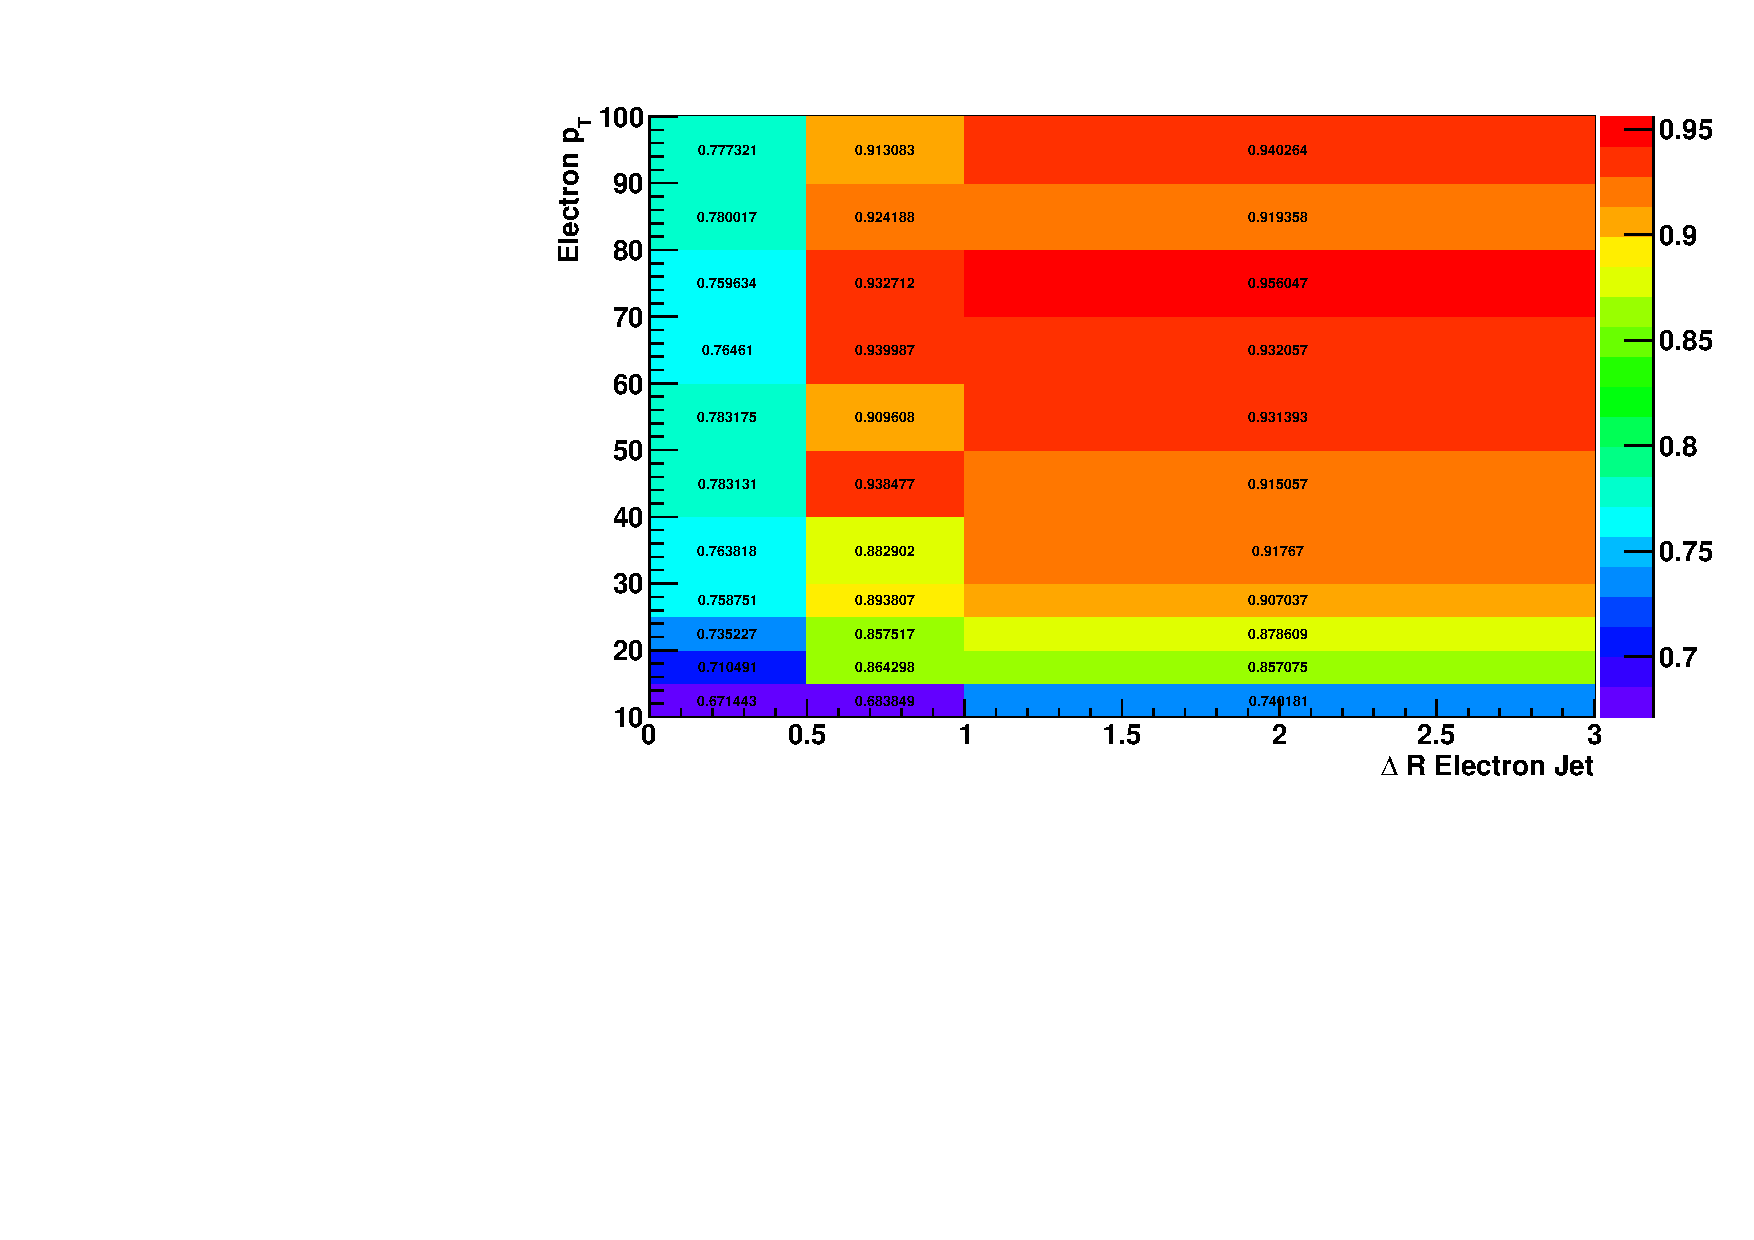
\includegraphics[width=.90\textwidth]{lostlepton/plots/Elec_Reco.pdf}\\
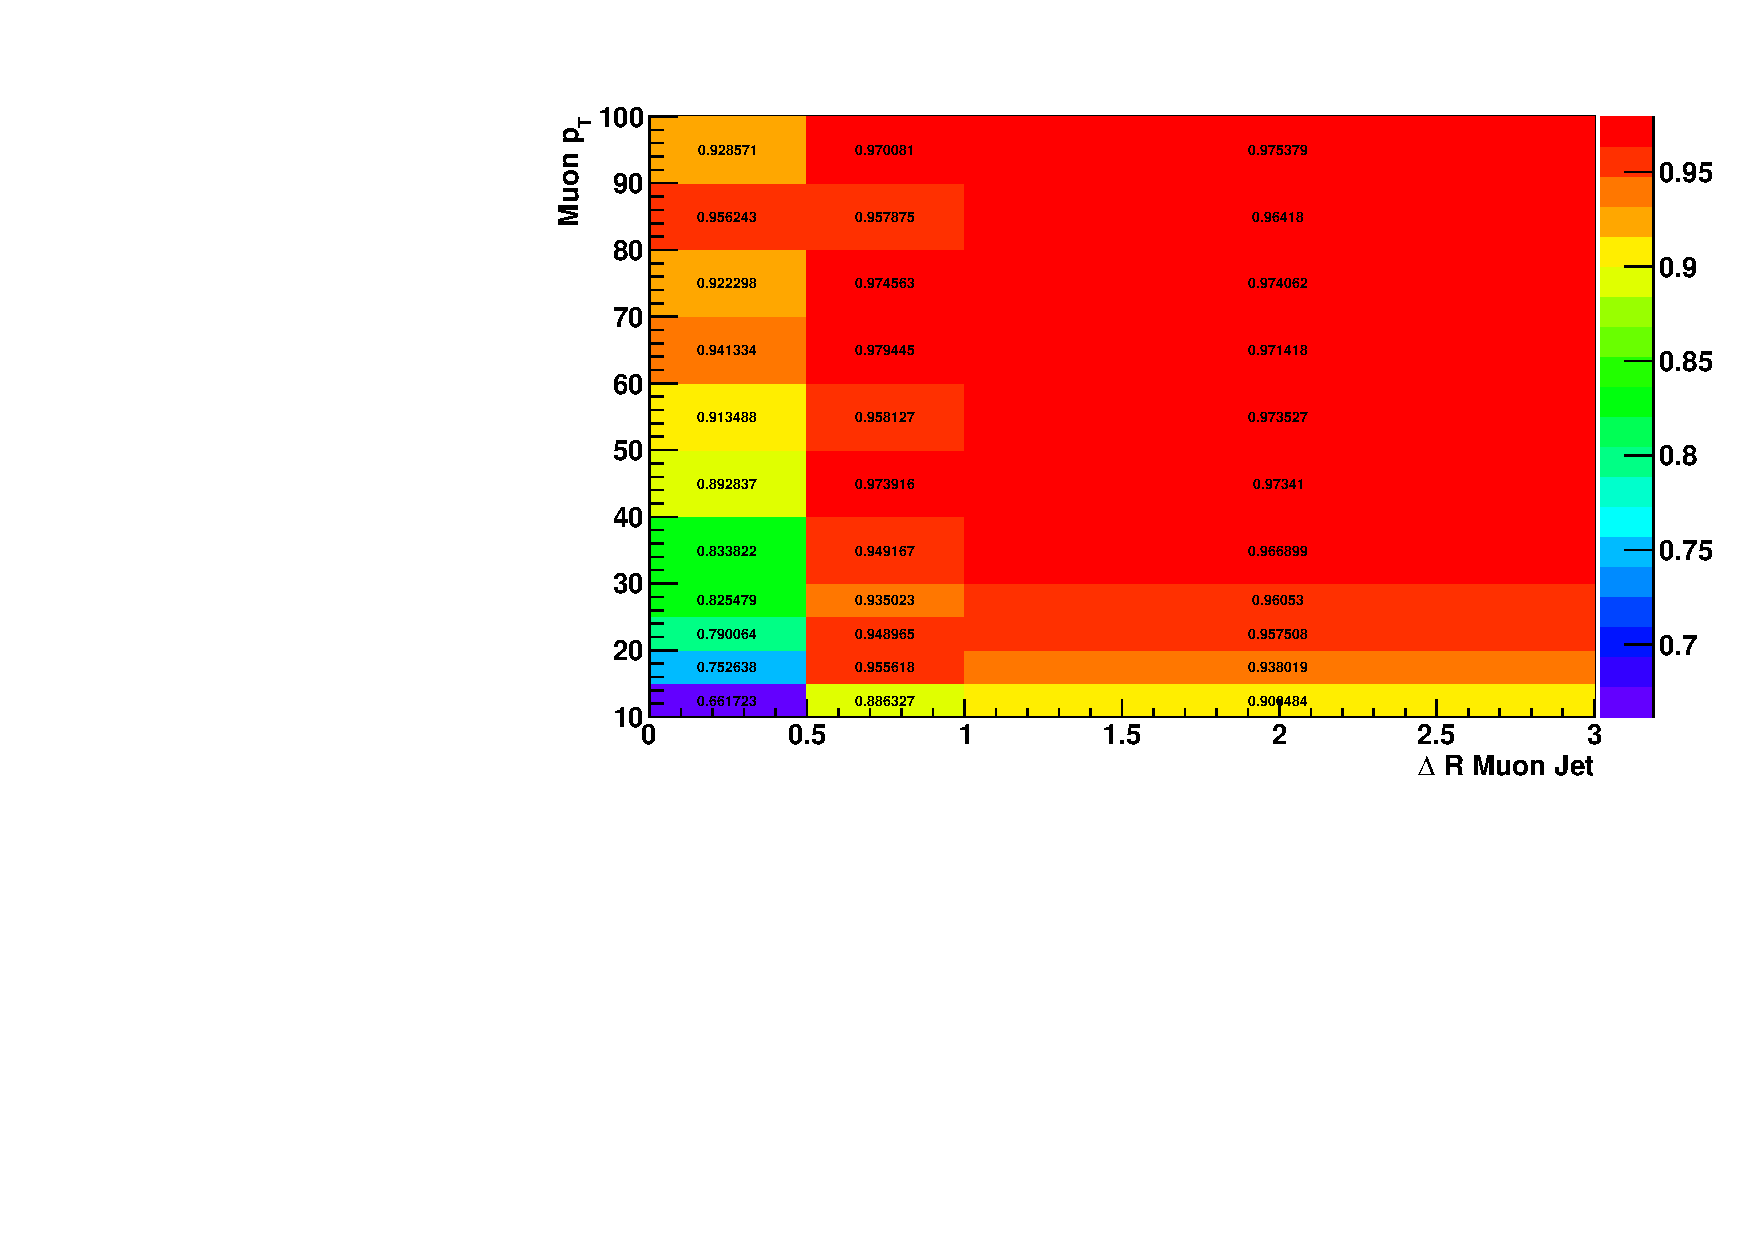
\includegraphics[width=.90\textwidth]{lostlepton/plots/Muon_Reco.pdf}\\
%\includegraphics[angle=0,width=0.5\textwidth]{wtop_lostlepton_figures/MHTMHT_r}&
%\includegraphics[angle=0,width=0.5\textwidth]{wtop_lostlepton_figures/HTHT_r}
%%(a)&(b)\\
\end{tabular}
\end{center}
\caption{These plots show the electron and $\mu$ reconstruction efficiencies obtained from MC.
}
\label{fig:reco_eff}
\end{figure}
%Fig. \ref{fig:not_reco} shows the distribution of not reconstructed  the right and not reconstructed muons on the left for \ttbar on top and for \wpj on the bottom separately. Good agreement between MC truth and MC prediction can be observed.
\clearpage

\subsection{Not isolated leptons}
\label{sec:isolation}
When a lepton is reconstructed it also has to fulfill the isolation criteria to be identified as a prompt lepton.
The applied isolation criteria are discussed in Sec.~\ref{sec:event_selection}.\\
Leptons show a higher isolation dependency on their \pt and angular distance relative to the closest jet.
Leading to the chosen efficiency parameterization in $\frac{p_{t,lep}}{p_{t,jet}}$ and $\Delta R$ to the closest jet. Especially for $\Delta R$ below 0.5 rad and low $\pt$ the efficiencies decrease strongly. To achieve as much accuracy as possible the $\Delta R$ binning has been optimized. However the statistics of the $Z$-sample are very limited in very small $\Delta R$. Fig.\ref{fig:iso_eff} shows the isolation efficiencies for electrons and $\mu$.
% iso eff
\begin{figure}[tbhn]
\begin{center}
\begin{tabular}{c}
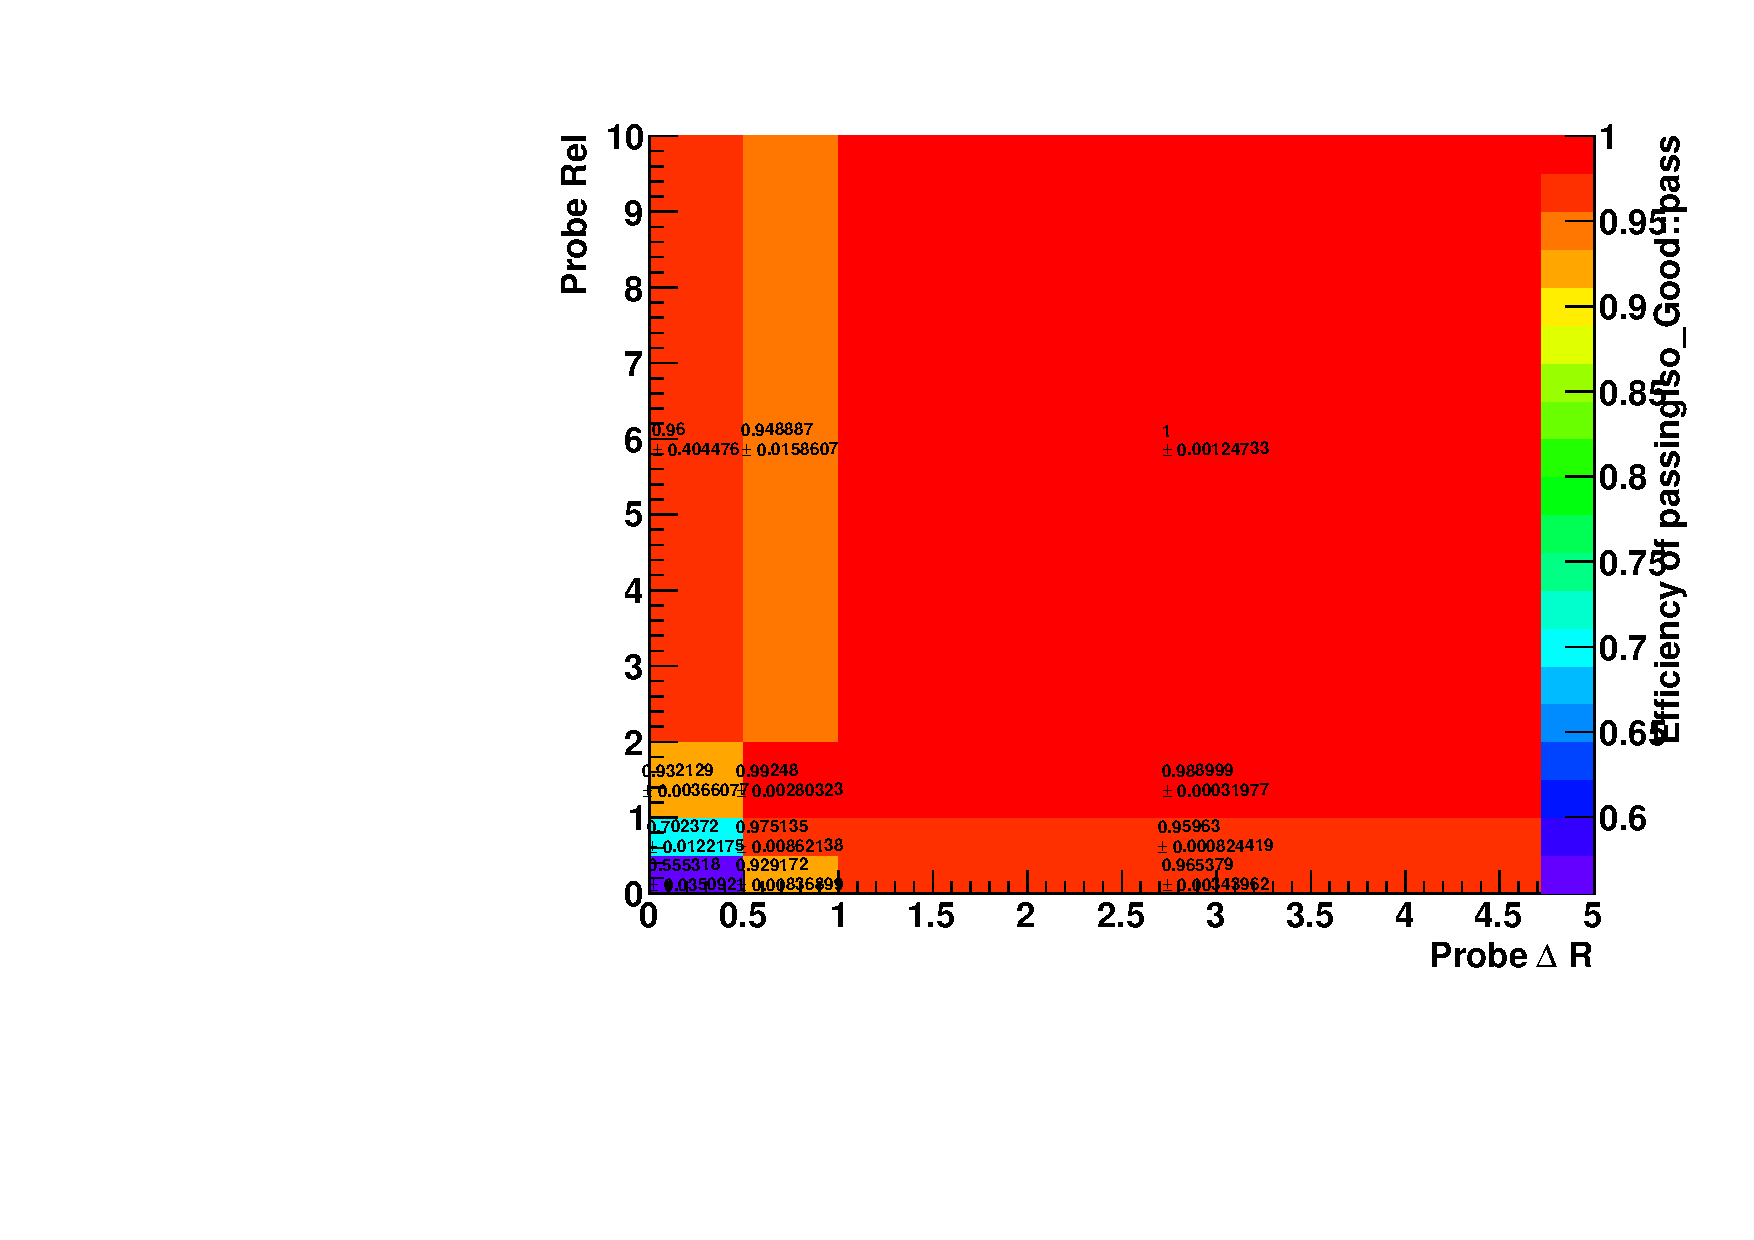
\includegraphics[width=.85\textwidth]{lostlepton/plots/Elec_Iso.pdf}\\
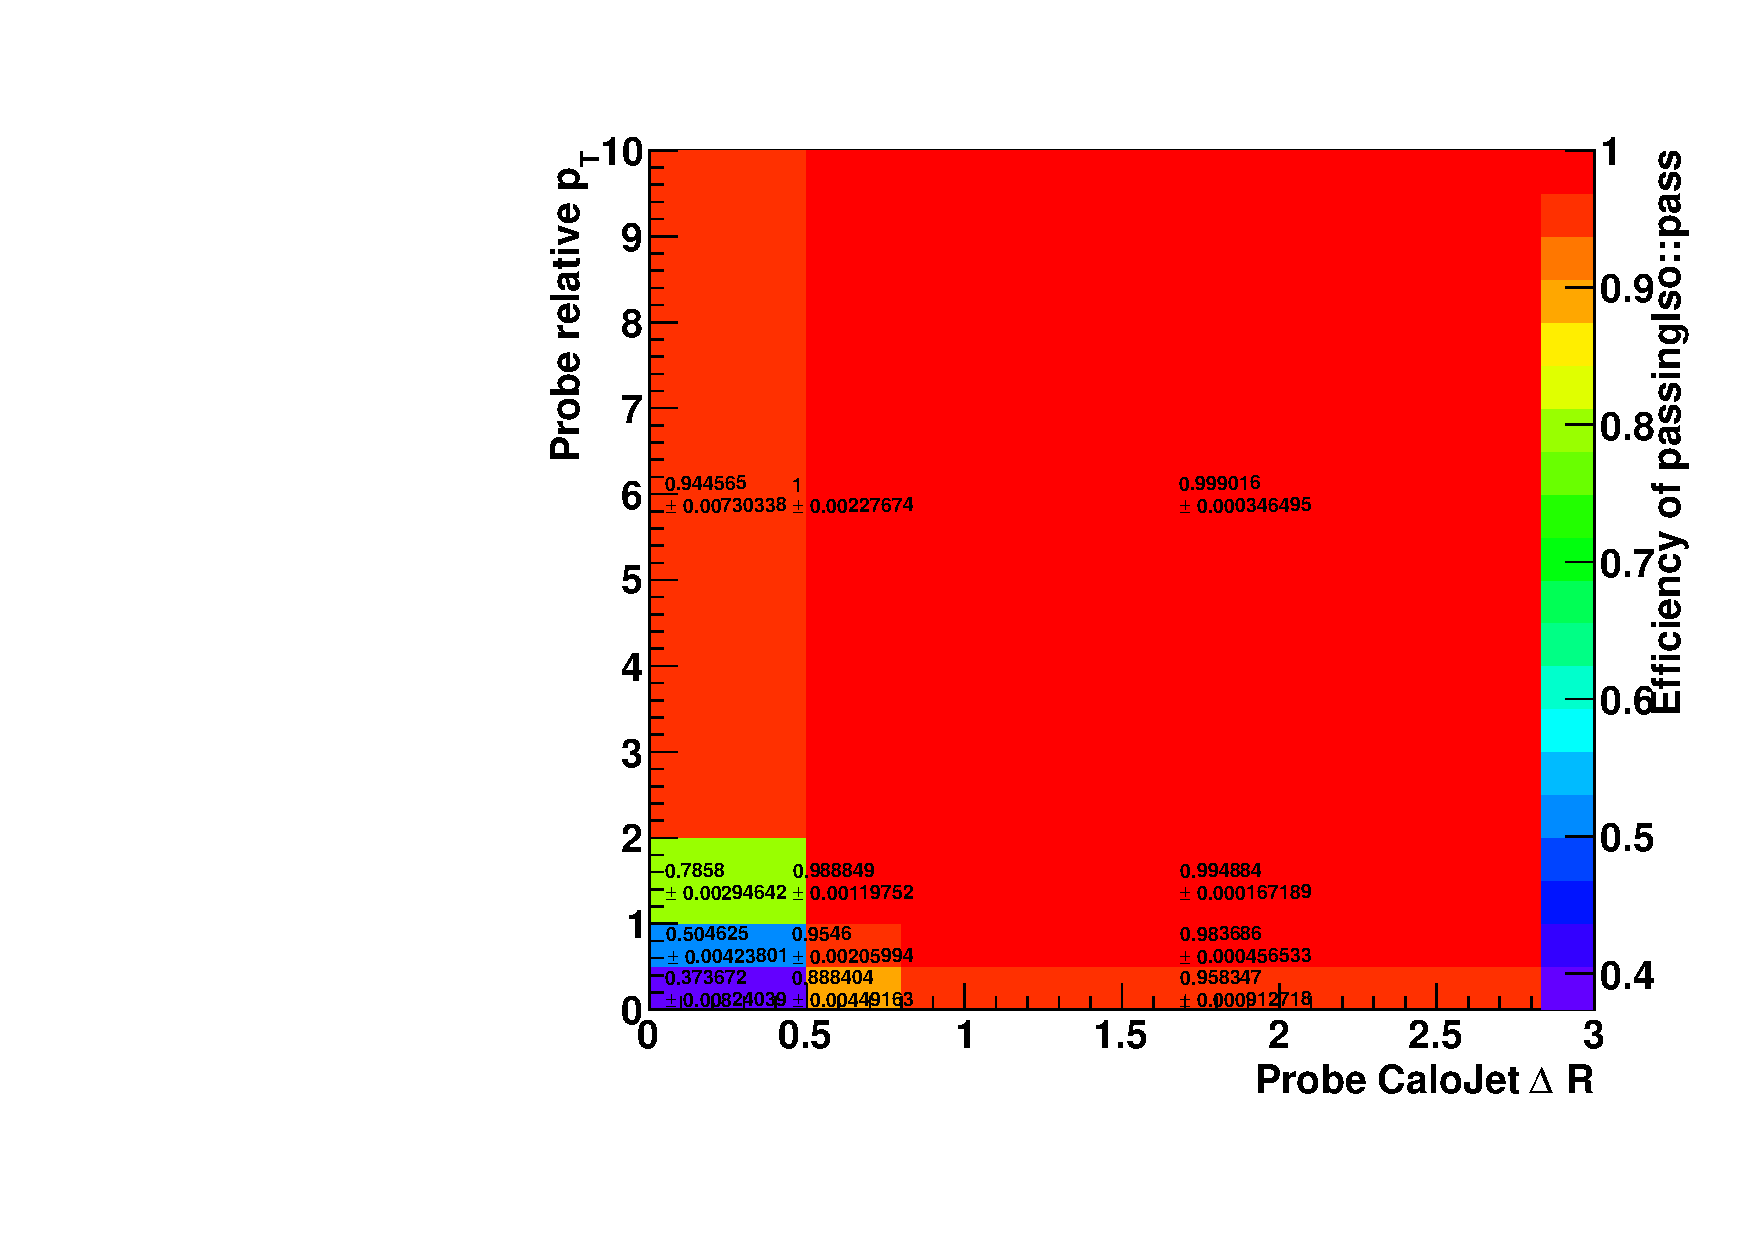
\includegraphics[width=.85\textwidth]{lostlepton/plots/Muon_Iso.pdf}\\
%\includegraphics[angle=0,width=0.5\textwidth]{wtop_lostlepton_figures/MHTMHT_r}&
%\includegraphics[angle=0,width=0.5\textwidth]{wtop_lostlepton_figures/HTHT_r}
%%(a)&(b)\\
\end{tabular}
\end{center}
\caption{These plots show the electron and $\mu$ isolation efficiencies calculated with a Tag\&Probe method.
}
\label{fig:iso_eff}
\end{figure}


\clearpage



\section{Closure tests and prediction on data}
\label{sec:closure_test}
Closure tests are a useful instrument of validating data driven methods on MC. For background estimations the prediction based on the MC control sample, labeled Data-driven Prediction from MC, is compared to the expected lost-leptons from MC, labeled MC expectation, in the signal region. Only statistical uncertainties are applied, since systematic uncertainties cancel within such a closure test.\\
One basic assumption of this method is that the topology of the CS and the signal sample do not differ considerable. The main search variables \HT and \MHT along with the number of primary vertices (see Sec.~\ref{sec:pileup})  are investigated to validate this assumption.\\ 
The closer test for the \HT and \MHT can be seen in Fig.~\ref{fig:closure}. Good agreement in shape can be observed. Tab.~\ref{tab:mc_closureA} contains the numbers of the Data-driven prediction on MC events compared to MC expectation for \ttbar and \wpj separately for the baseline selection. Also here good agreement can be observed. Despite a statistical significant discrepancy for the not reconstructed muons for \wpj and the not isolated muons for \ttbar, leading to an observed 4\% underestimation, called non-closure, for which a correction factor is applied on data, the closure tests show that the topology of the events including lost leptons and the CS events agree well and that the assumption of similar topologies is valid for the baseline selection. The observed underestimation is discussed in the following.\\
\begin{table}[htb]
\begin{center}
    \begin{tabular}{|l|ll|ll|}
        \hline
        ~    				& \ttbar expectation   & \ttbar predic.    & \wpj expectation       & \wpj predic.    \\ \hline %& combined truth &combined predic.\\ \hline
        $\mu$, out of acceptance  	& $51.1\pm 0.9$ & $47.7\pm 0.4$    & $79.6\pm 2.0$ & $80.3\pm 0.9$ \\ \hline %&  $130.7\pm 2.3$& $128.0\pm 1.0$\\ \hline
        $\mu$, not reconstructed  	& $16.6\pm 0.5$ & $17.4\pm 0.3$    & $18.3\pm 0.9$ & $15.7\pm 0.3$ \\ \hline  %&  $35.0\pm 1.1$& $33.1\pm 0.4$\\ \hline
        $\mu$, not isolated 		& $34.6\pm 0.7$ & $27.1\pm 0.6$    & $25.9\pm 1.1$ & $25.9\pm 1.1$ \\ \hline \hline%&  $60.5\pm 1.3$& $53.0\pm 1.0$\\ \hline \hline
        $e$, out of acceptance		& $57.1\pm 0.9$ & $55.5\pm 0.5$    & $88.4\pm 2.1$ & $90.8\pm 1.1$ \\ \hline%&  $145.5\pm 2.3$& $146.3\pm 1.2$\\ \hline
       	$e$, not reconstructed 		& $35.4\pm 0.7$ & $35.3\pm 0.4$    & $50.1\pm 1.5$ & $46.1\pm 0.7$ \\ \hline%&  $85.4\pm 1.7$& $81.5\pm 0.8$\\ \hline
        $e$, not isolated		& $28.5\pm 0.6$ & $21.0\pm 0.4$    & $21.5\pm 1.0$ & $21.2\pm 0.6$ \\ \hline \hline %&  $50.0\pm 1.2$& $42.2\pm 0.8$\\ \hline \hline
	total				& $219.2\pm 1.8$ & $204.1\pm 2.3$  & $285.0\pm 3.7$ & $280.0\pm 4.0$ \\ %&  $504.2\pm 4.1$& $484.1\pm 4.6$\\
        \hline
    \end{tabular}
\caption{This table shows the prediction on MC vs the expected events from MC. The numbers are scaled to \lumi.\label{tab:mc_closureA}}
\end{center}
\end{table}
Fig.~\ref{fig:closure_sepTTbar} and Fig.~\ref{fig:closure_sepW} show the closure test for \HT and \MHT for \ttbar and \wpj separately. For \wpj both the \MHT and \HT distribution agree well in shape. For \ttbar the \HT distribution agrees also well but the \MHT distribution shows an increasing under-prediction. Further closer tests have been done for the \ttbar \MHT distribution separately for not isolated, not reconstructed or out of the detector acceptance leptons.\\ %For completeness the closure plots for \wpj are also attached in the appendix.\\ 
The observed increasing under-prediction arises from the contribution of not isolation leptons and is passed to the other contribution since they also depend on the muon isolation efficiency (see Sec.~\ref{sec:ll_prediction}.\\
This observation can be understood by considering the boost of the \ttbar system at larger \MHT. The increasing boost of the top quarks leads to a shrinking angular distance, $\Delta R$, between the $b$-jet and the $W$. The final decay products, the lepton and the $\nu$, are also boosted resulting in an increased \MHT and smaller angular distance $\Delta R$ between the lepton and the $b$-jet. The under-prediction arises now since the isolation efficiencies decrease strongly with $\Delta R$ approaching 0 and as stated in Sec.~\ref{sec:tag_probe} it is not possible to parametrize the binning of the efficiencies $\Delta R$ any smaller. This incapability of the method to account for this extreme boosted systems with this very small $\Delta R$ is unavoidably and results in the observed increasing non-closure with increasing \MHT.\\
For the \wpj sample a similar dependency is not expected because there is no correlation between \MHT and $\Delta R$.\\ 
This well understood systematic under-prediction justifies the correction factor of 4\% applied on data together with an additional uncertainty, introduced in Sec.~\ref{sec:uncertainties}, covering this dependency and other possible remaining differences in the closure, eg. the observed non-closure for the not reconstructed muons in the \wpj sample.\\
Fig.~\ref{fig:reco_acc_combined} shows the \ttbar and \wpj combined closure test for the out of acceptance and not reconstructed fraction for electrons and muons separately. Together with the numbers from Tab.~\ref{tab:mc_closureA} one can observe good agreement for the not reconstructed and out of acceptance contribution.\\
Since it is not possible to separate the lost-lepton background from the other backgrounds, equivalent closure tests on data can not be done. Instead the $\mu$ CS from MC and data, and the prediction on data and MC are compared, as can be seen in Fig.~\ref{fig:LostLepton_MuCS_data_MC} and Fig.~\ref{fig:predicDataMC}. \\
For both distributions a good agreement in shape can be observed. However both the control sample and the prediction show a significant difference (see Tab.~\ref{tab:LostLeptonCompare}) but the idea of data-driven background estimation is to be independent from MC. The observed differences are expected to origin from deficiencies in the MC simulation.\\ 
Tab.~\ref{tab:LostLeptonCompare} contains the event yields on data, the Data-driven Prediction from MC and the MC Expectation. The prediction for the different search regions on data (defined in Sec.~\ref{sec:event_selection}) including all systematics uncertainties (discussed in Sec.~\ref{sec:uncertainties}) are shown in Tab.~\ref{tab:LostLeptonResult1}.
\begin{table}[hbt]
\selectfont
\begin{centering}
\caption[]{This table contains the final event yield for the lost-lepton background for the baseline selection on data and Data-driven Prediction from MC together with MC Expectation\footnote{The observed MC events are scaled to the full luminosity of \lumi.}. All uncertainties are included for the prediction on data. For the MC Expectation jet energy scale and luminosity uncertainties are applied and for the prediction on MC only statistical uncertainties are included.\label{tab:LostLeptonCompare} } 

\hspace*{-4ex}
\begin{tabular}{|c|c|c|c|}
\hline
\			& Pred. & Stat. Error	& Tot. Sys.		\\
\hline 
prediction on data	&453.5	&$\pm 26.3$	&$^{+52.5}_{-53.4}$	\\
MC Expectation	    	&545.8  &$\pm 4.5$	&$^{+50.4}_{-51.1}$	\\
Data-driven Prediction from MC	&524.1	&$\pm 5.0$	&	\\ \hline

\end{tabular}
\par\end{centering}
\end{table}

% 
\begin{figure}[tbhn]
\begin{center}
\begin{tabular}{cc}
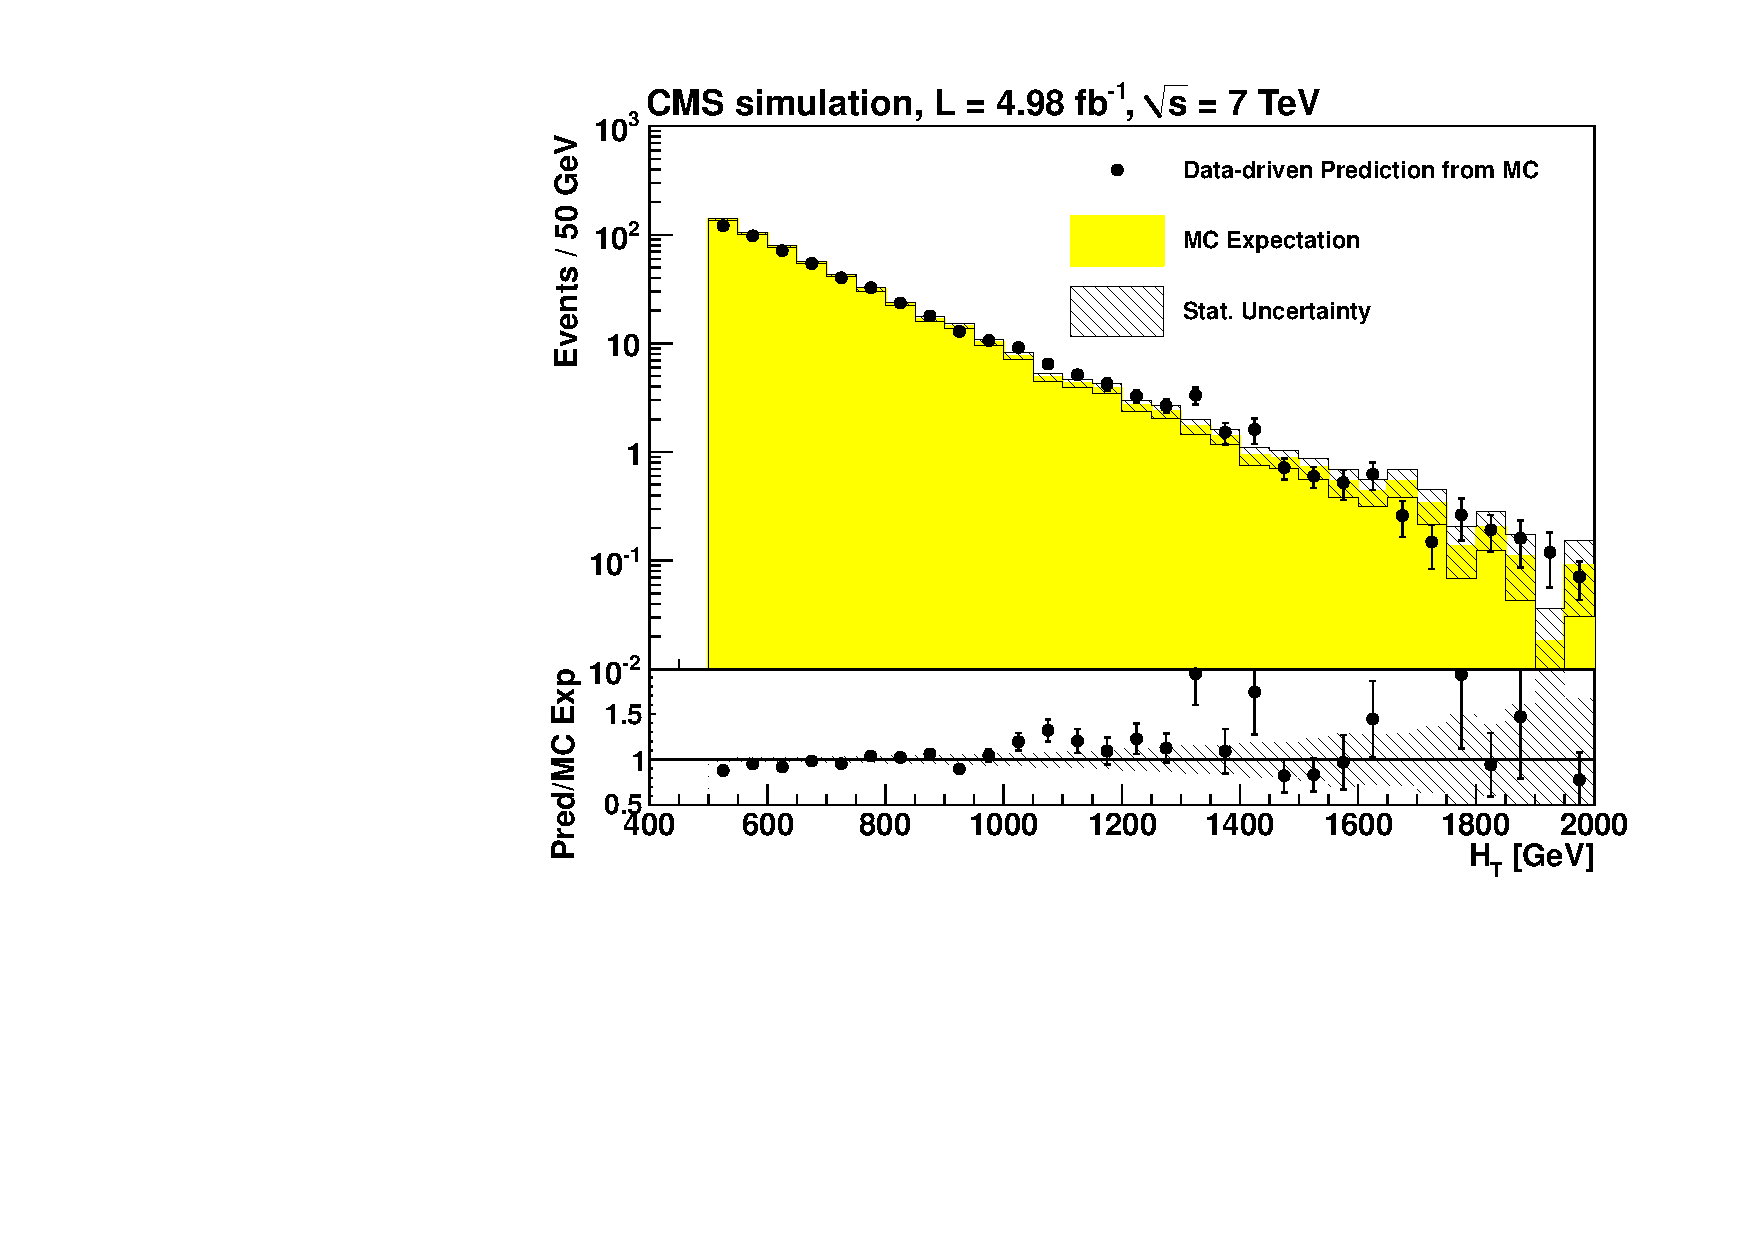
\includegraphics[width=0.90\textwidth]{lostlepton/plots/ANplots/Closure_HT.pdf}\\
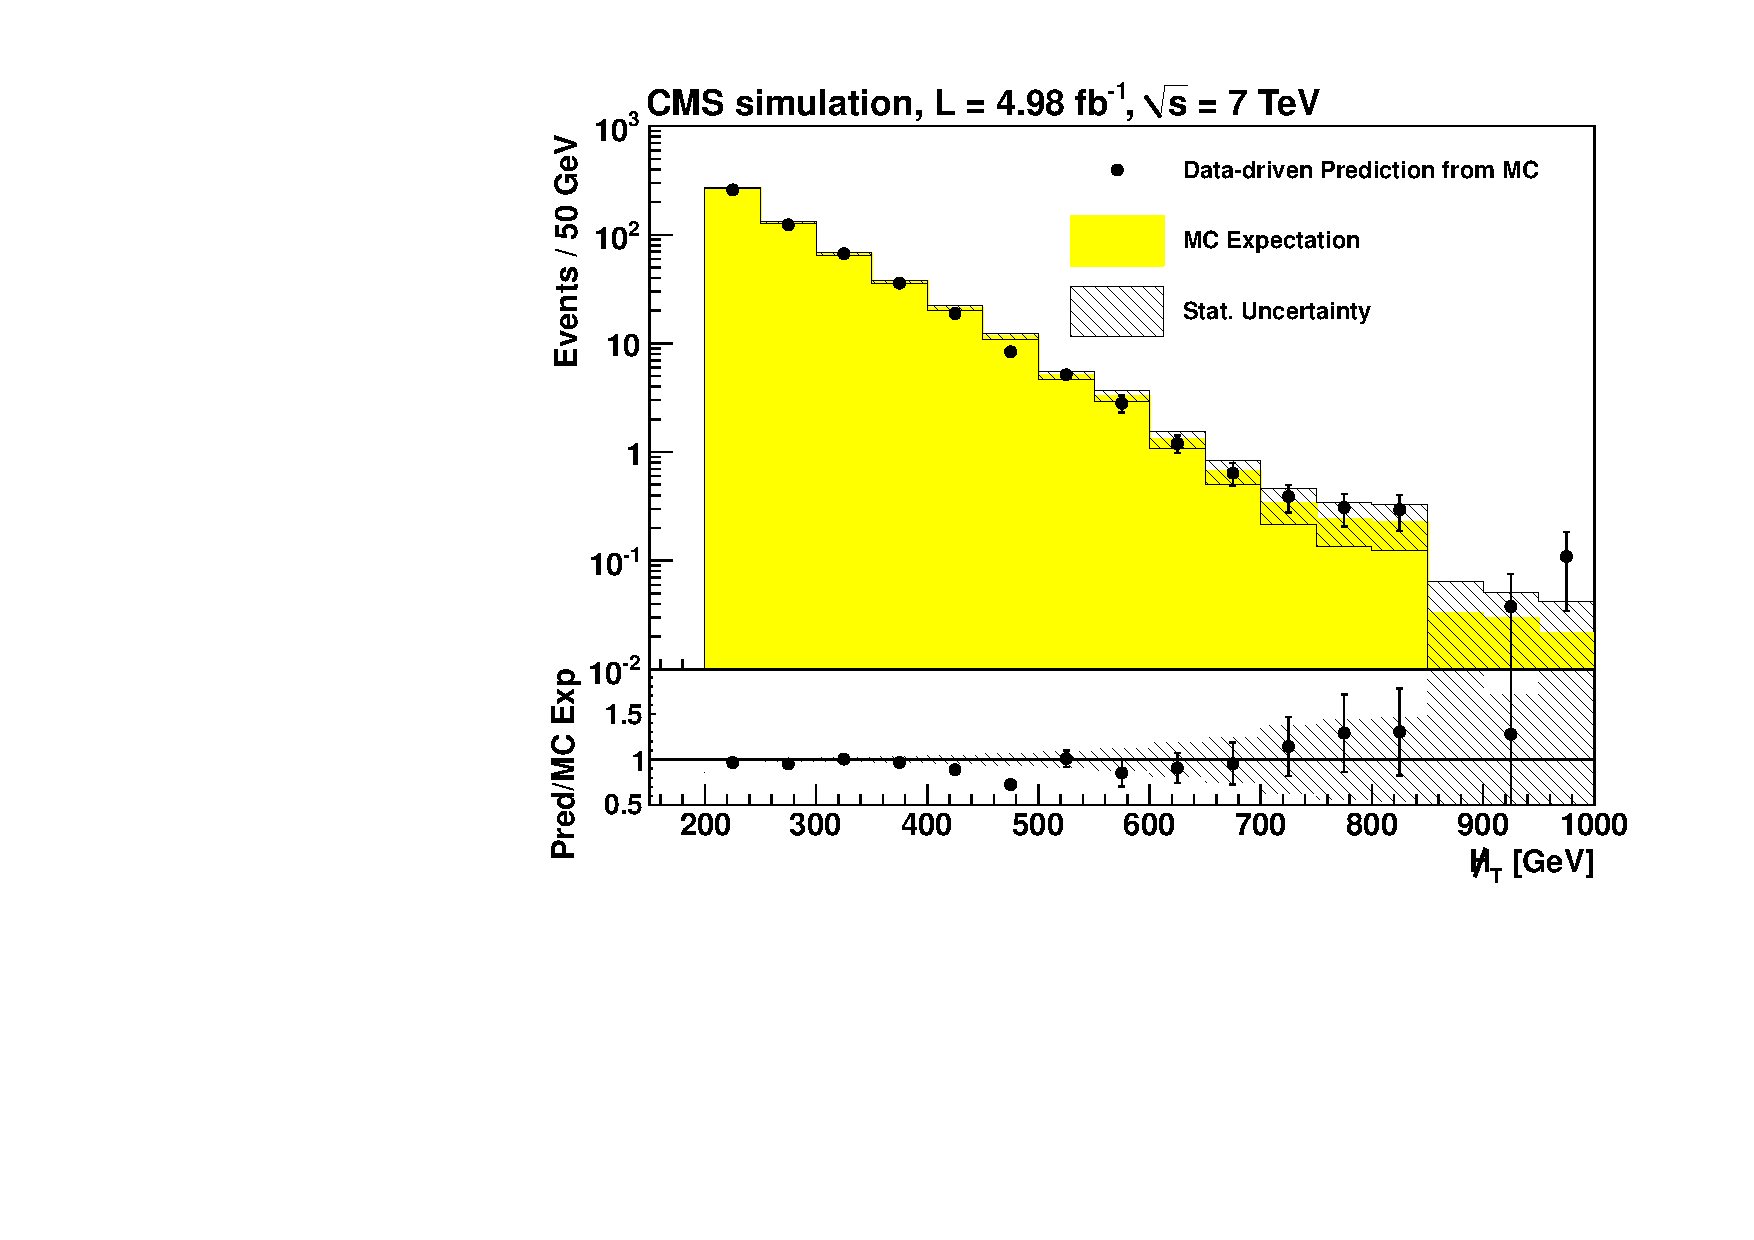
\includegraphics[width=0.90\textwidth]{lostlepton/plots/ANplots/Closure_MHT.pdf}

%\includegraphics[angle=0,width=0.5\textwidth]{wtop_lostlepton_figures/MHTMHT_r}&
%\includegraphics[angle=0,width=0.5\textwidth]{wtop_lostlepton_figures/HTHT_r}
%%(a)&(b)\\
\end{tabular}
\end{center}
\caption{These plots show the closure test for the \HT and \MHT baseline selection for the total lost-lepton background. The estimated lost-leptons are called Data-driven Prediction from MC, which refers to \ttbar and \wpj events combined and the observed lost-leptons are referred to as MC expectation.}
\label{fig:closure}
\end{figure}
%The method is tested in different distributions, the important search variable \MHT and \HT of course but also for jet-multiplicity and number of primary vertices(see sec. \ref{sec:pileup}). For validation the numbers in table \ref{tab:mc_closure} and the separated plots are used.
%The closure test has been done for \ttbar and \wpj separately and also for all the different contribution to the total lost lepton background. in the following each sample is discussed separately and the closure is interpreted.





% prediction on data vs mc
\begin{figure}[tbhn]
\begin{center}
\begin{tabular}{cc}
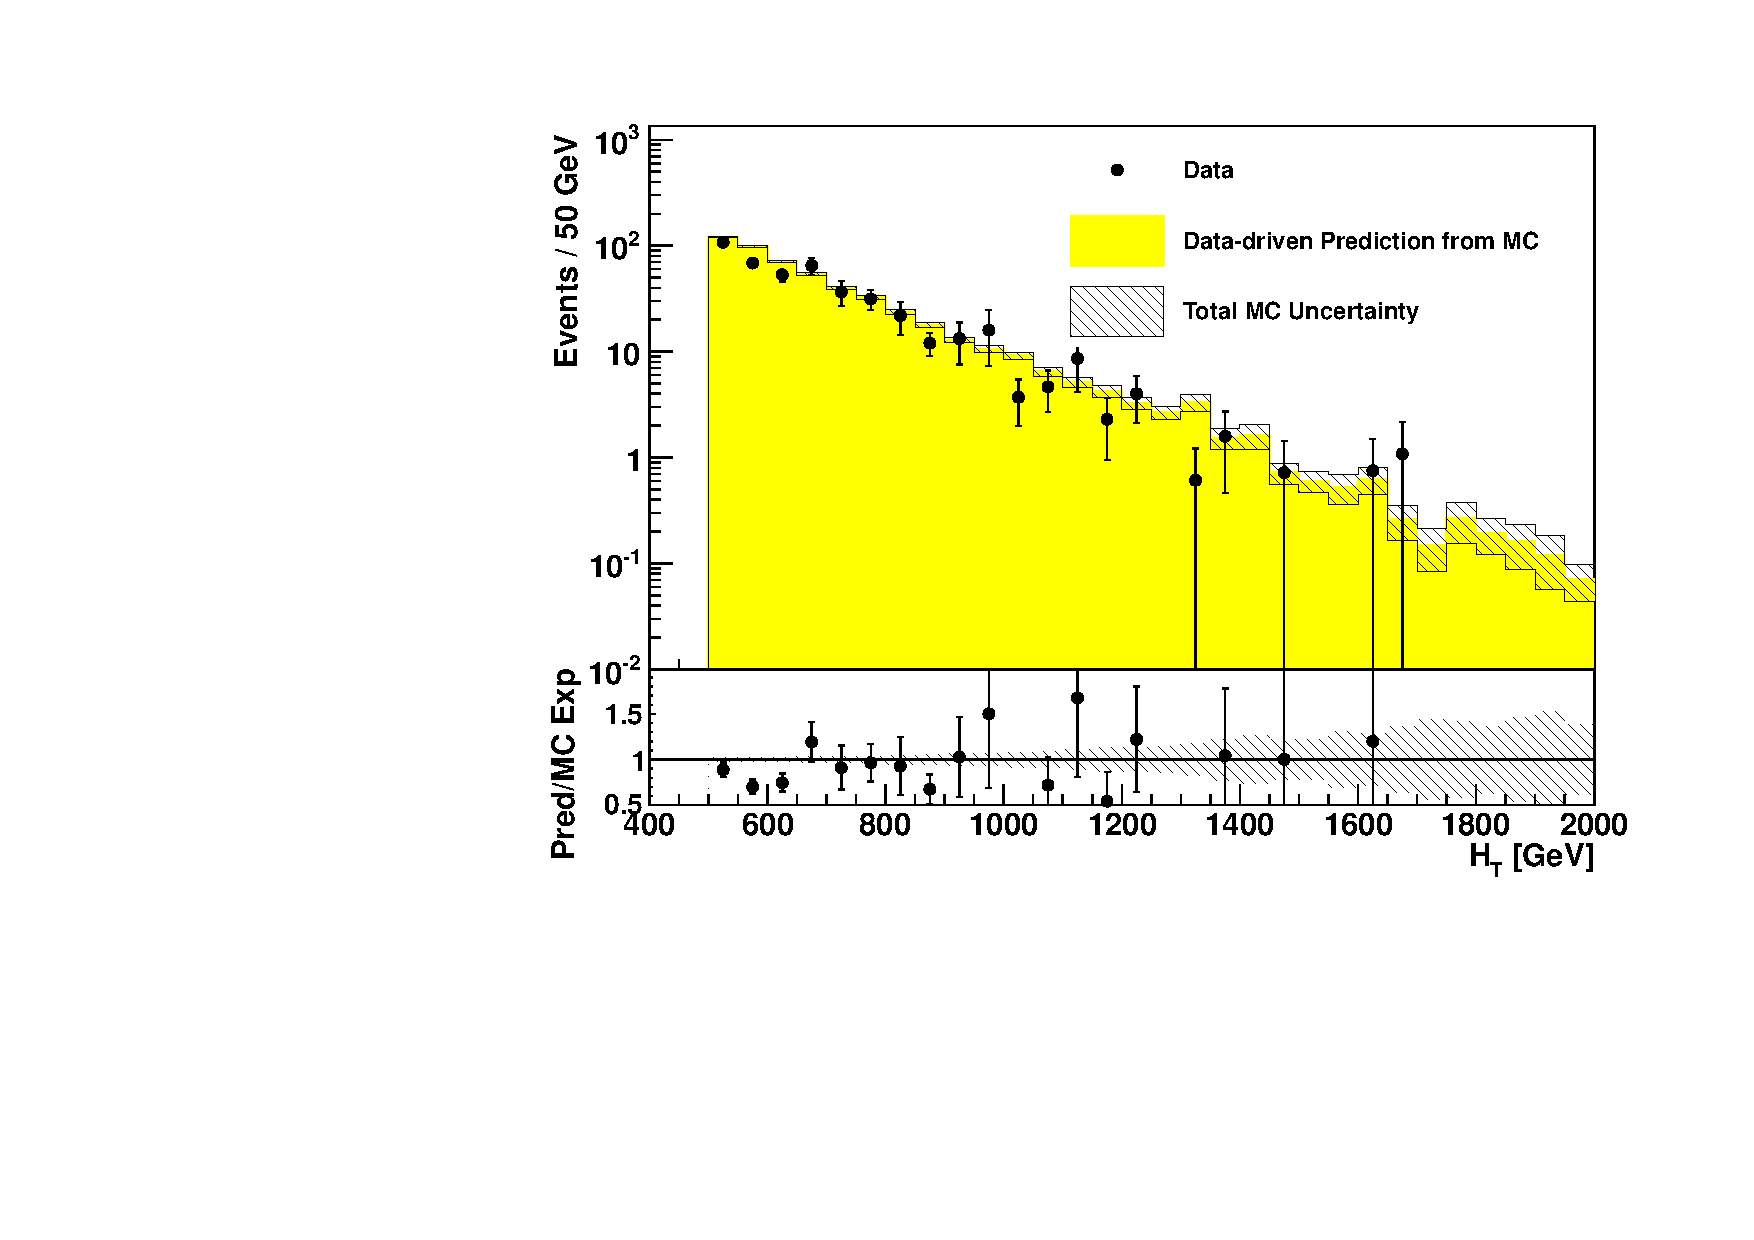
\includegraphics[width=0.90\textwidth]{lostlepton/plots/closure/DataVsMCPredictionHT.pdf}\\
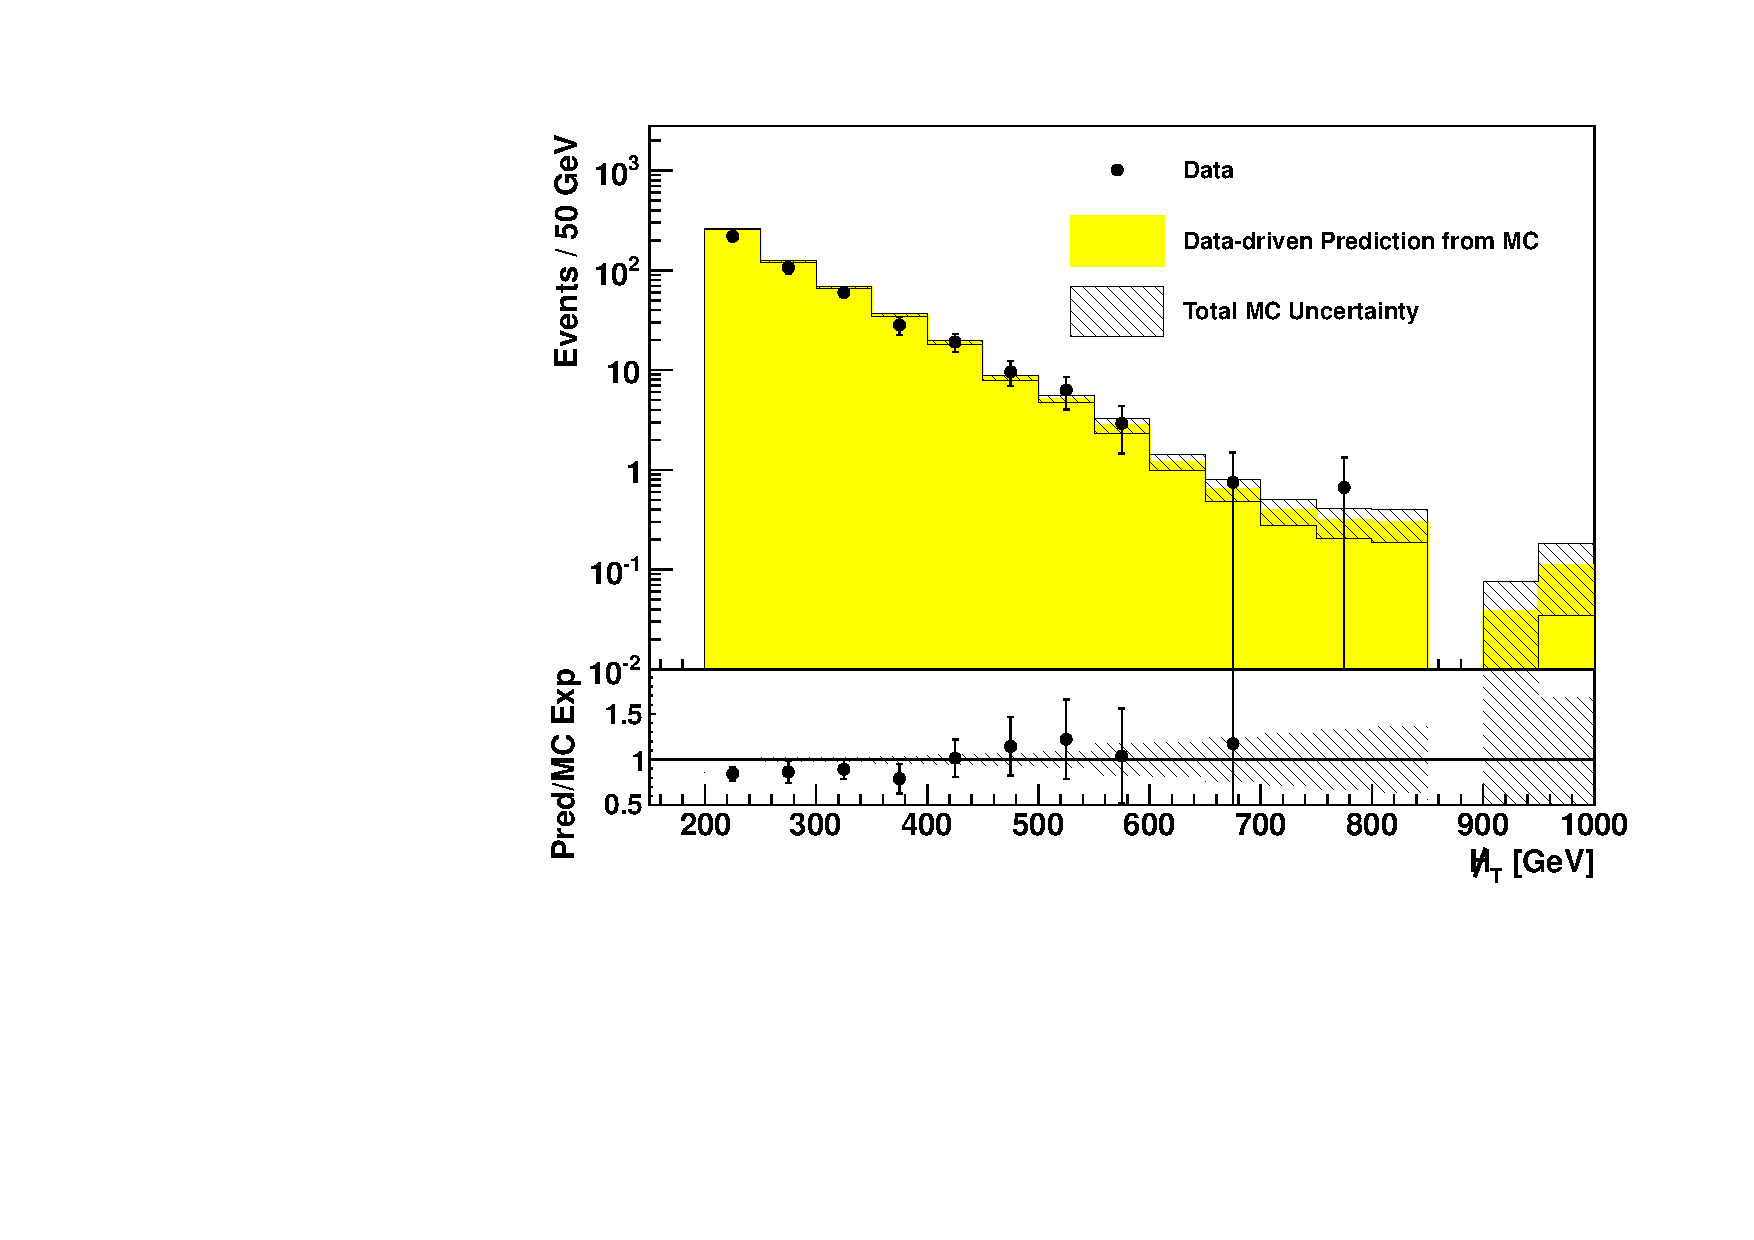
\includegraphics[width=0.90\textwidth]{lostlepton/plots/closure/DataVsMCPredictionMHT.pdf}

%\includegraphics[angle=0,width=0.5\textwidth]{wtop_lostlepton_figures/MHTMHT_r}&
%\includegraphics[angle=0,width=0.5\textwidth]{wtop_lostlepton_figures/HTHT_r}
%%(a)&(b)\\
\end{tabular}
\end{center}
\caption{Comparison of the prediction on data vs. the prediction on MC (\ttbar and \wpj combined) for the \HT (on the right) and the \MHT (on the left) distribution. For the data prediction all uncertainties are shown while for the MC prediction only statistical uncertainties are shown. The shapes agree well within the uncertainties.}
\label{fig:predicDataMC}
\end{figure}


%\subsection{\wpj closure test}
%\label{wpj_closure}
%The overall closure for the \wpj sample shows a really good agreement in numbers (see tab. \ref{tab:mc_closure}) and shape (see fig. \ref{fig:wpj_closure}).

% leading jet pt and number of jets
%\begin{figure}[tbhn]
%\begin{center}
%\begin{tabular}{cc}
%\includegraphics[width=0.50\textwidth]{lostlepton/plots/closure/ttbar/Jet1PtClosure.pdf}
%\includegraphics[width=0.50\textwidth]{lostlepton/plots/closure/w/Jet1PtClosure.pdf}
%\includegraphics[angle=0,width=0.5\textwidth]{wtop_lostlepton_figures/MHTMHT_r}&
%\includegraphics[angle=0,width=0.5\textwidth]{wtop_lostlepton_figures/HTHT_r}
%%(a)&(b)\\
%\end{tabular}
%\end{center}
%\caption{This plots show a closure test for the \pt of the leading jet for \ttbar and \wpj. Good agreement of the shape as well as the ratio can be seen.
%}
%\label{fig:jet_closure}
%\end{figure}

% leading jet pt and number of jets
\begin{figure}[tbhn]
\begin{center}
\begin{tabular}{cc}
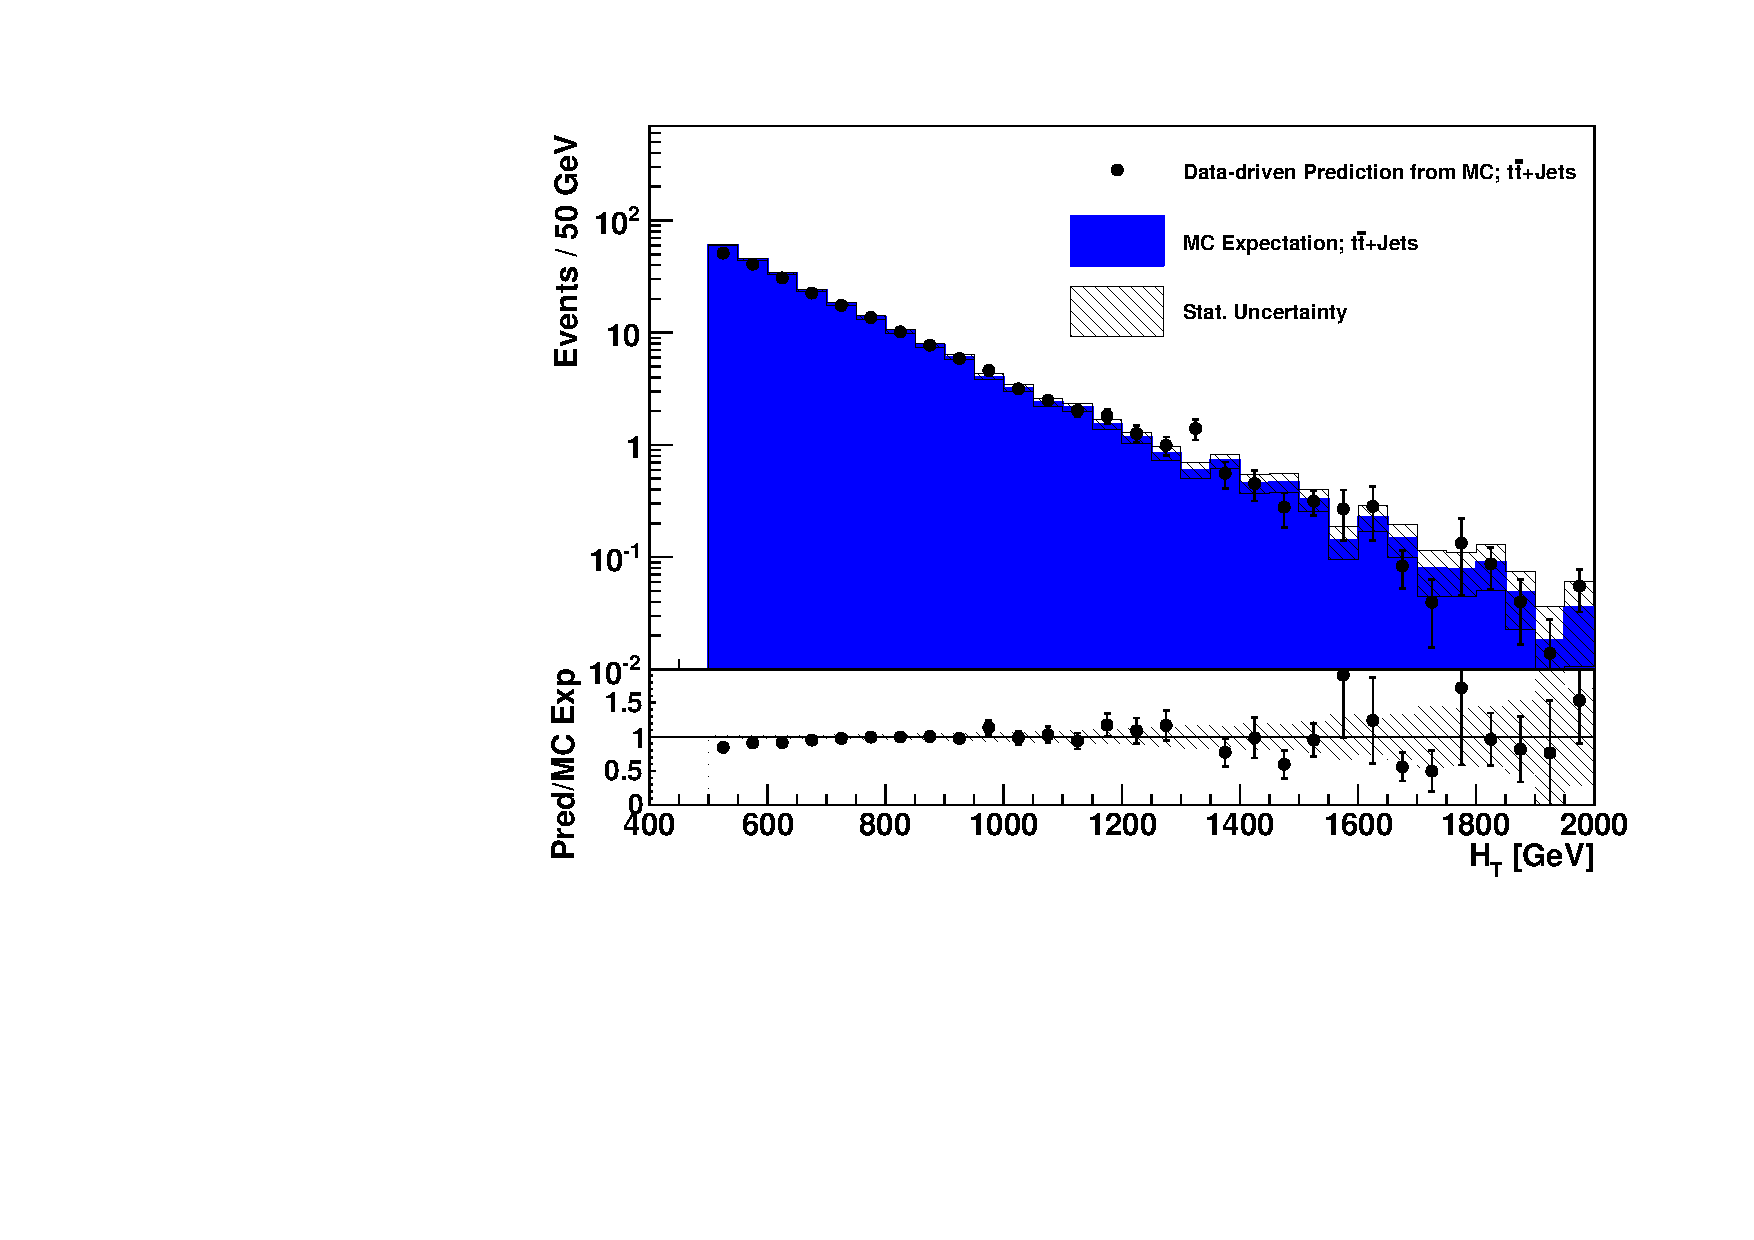
\includegraphics[width=0.90\textwidth]{lostlepton/plots/closure/HTttbar.pdf}\\
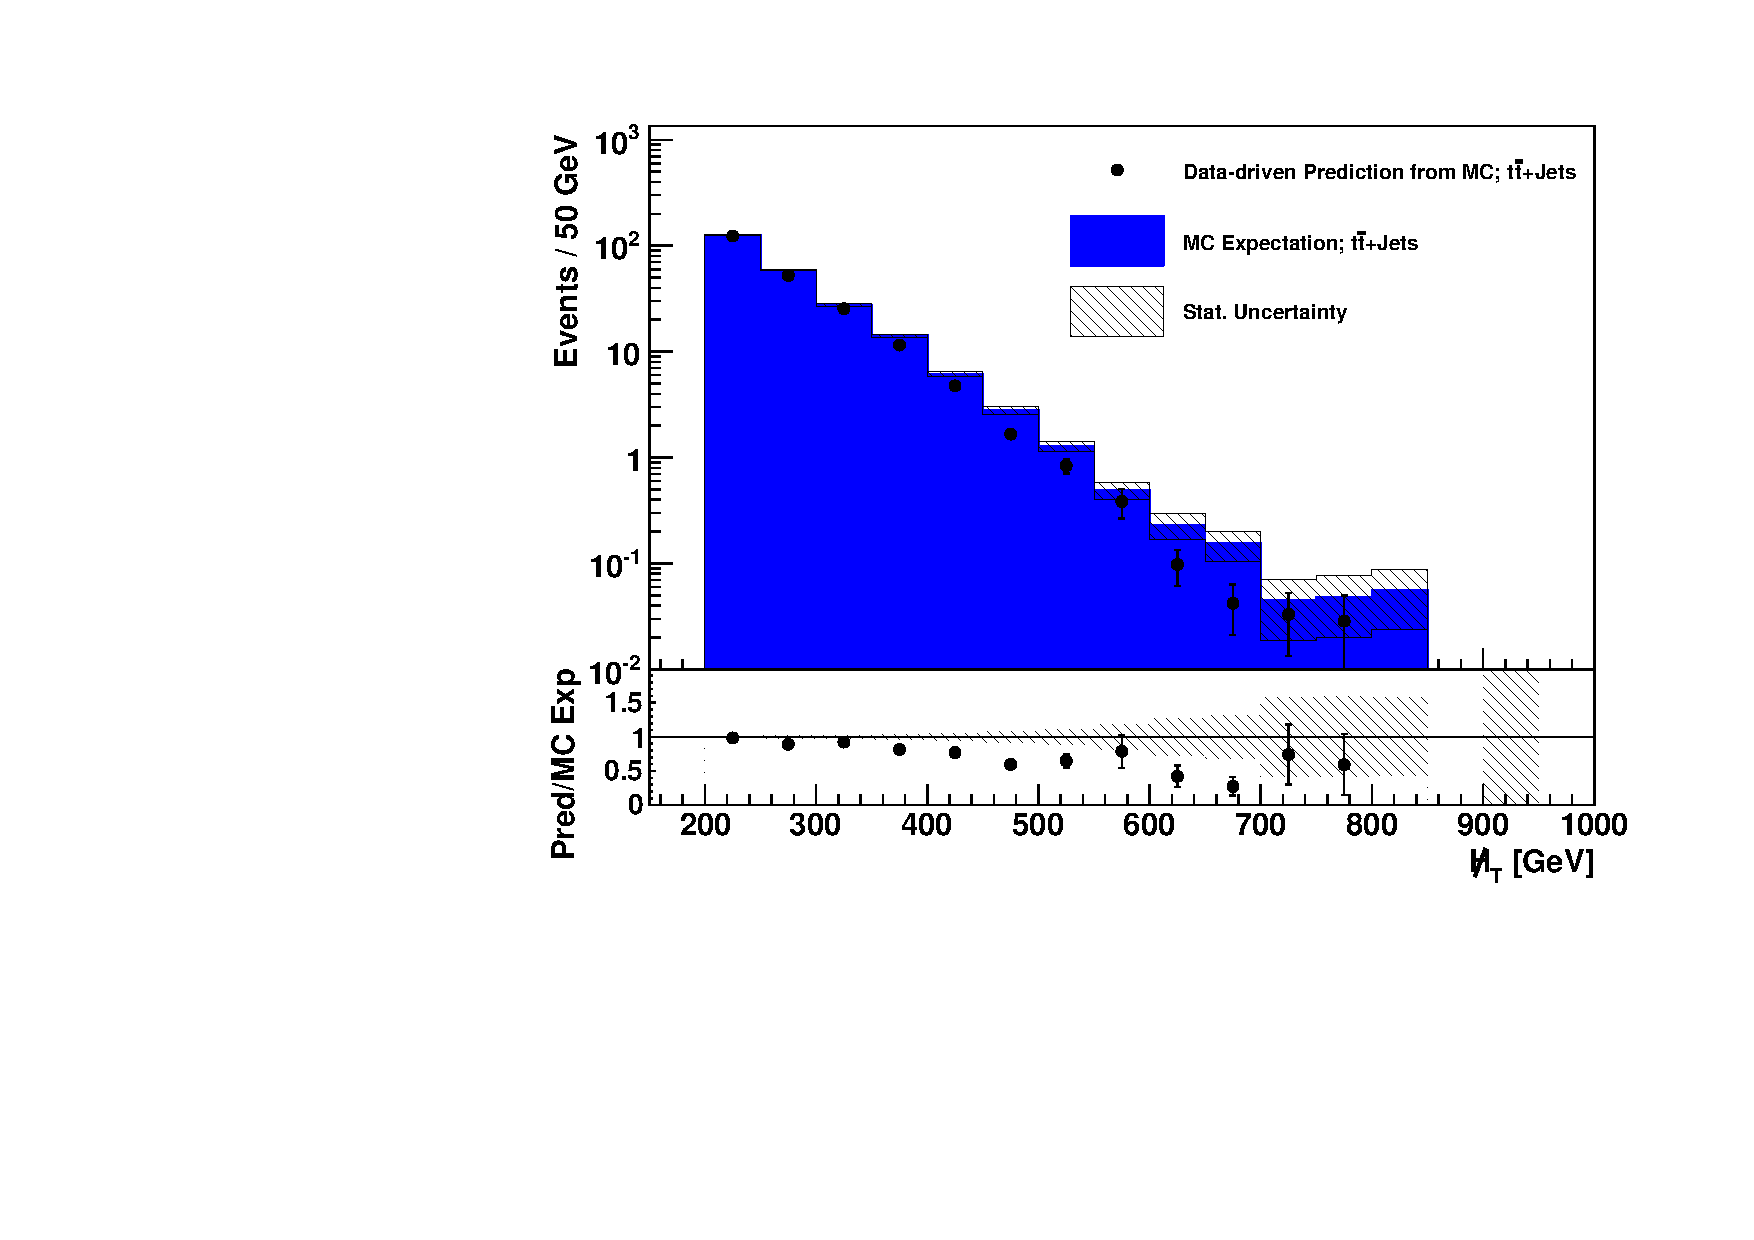
\includegraphics[width=0.90\textwidth]{lostlepton/plots/closure/MHTttbar.pdf}

%\includegraphics[angle=0,width=0.5\textwidth]{wtop_lostlepton_figures/MHTMHT_r}&
%\includegraphics[angle=0,width=0.5\textwidth]{wtop_lostlepton_figures/HTHT_r}
%%(a)&(b)\\
\end{tabular}
\end{center}
\caption{This plots show the closure test of the Data-driven Prediction from MC and the MC expectation for the \HT and \MHT distribution for \ttbar simulated events. Good agreement of the shape as well as the ratio can be seen. Only the \MHT distribution shows a significant discrepancy.
}
\label{fig:closure_sepTTbar}
\end{figure}
\begin{figure}[tbhn]
\begin{center}
\begin{tabular}{cc}

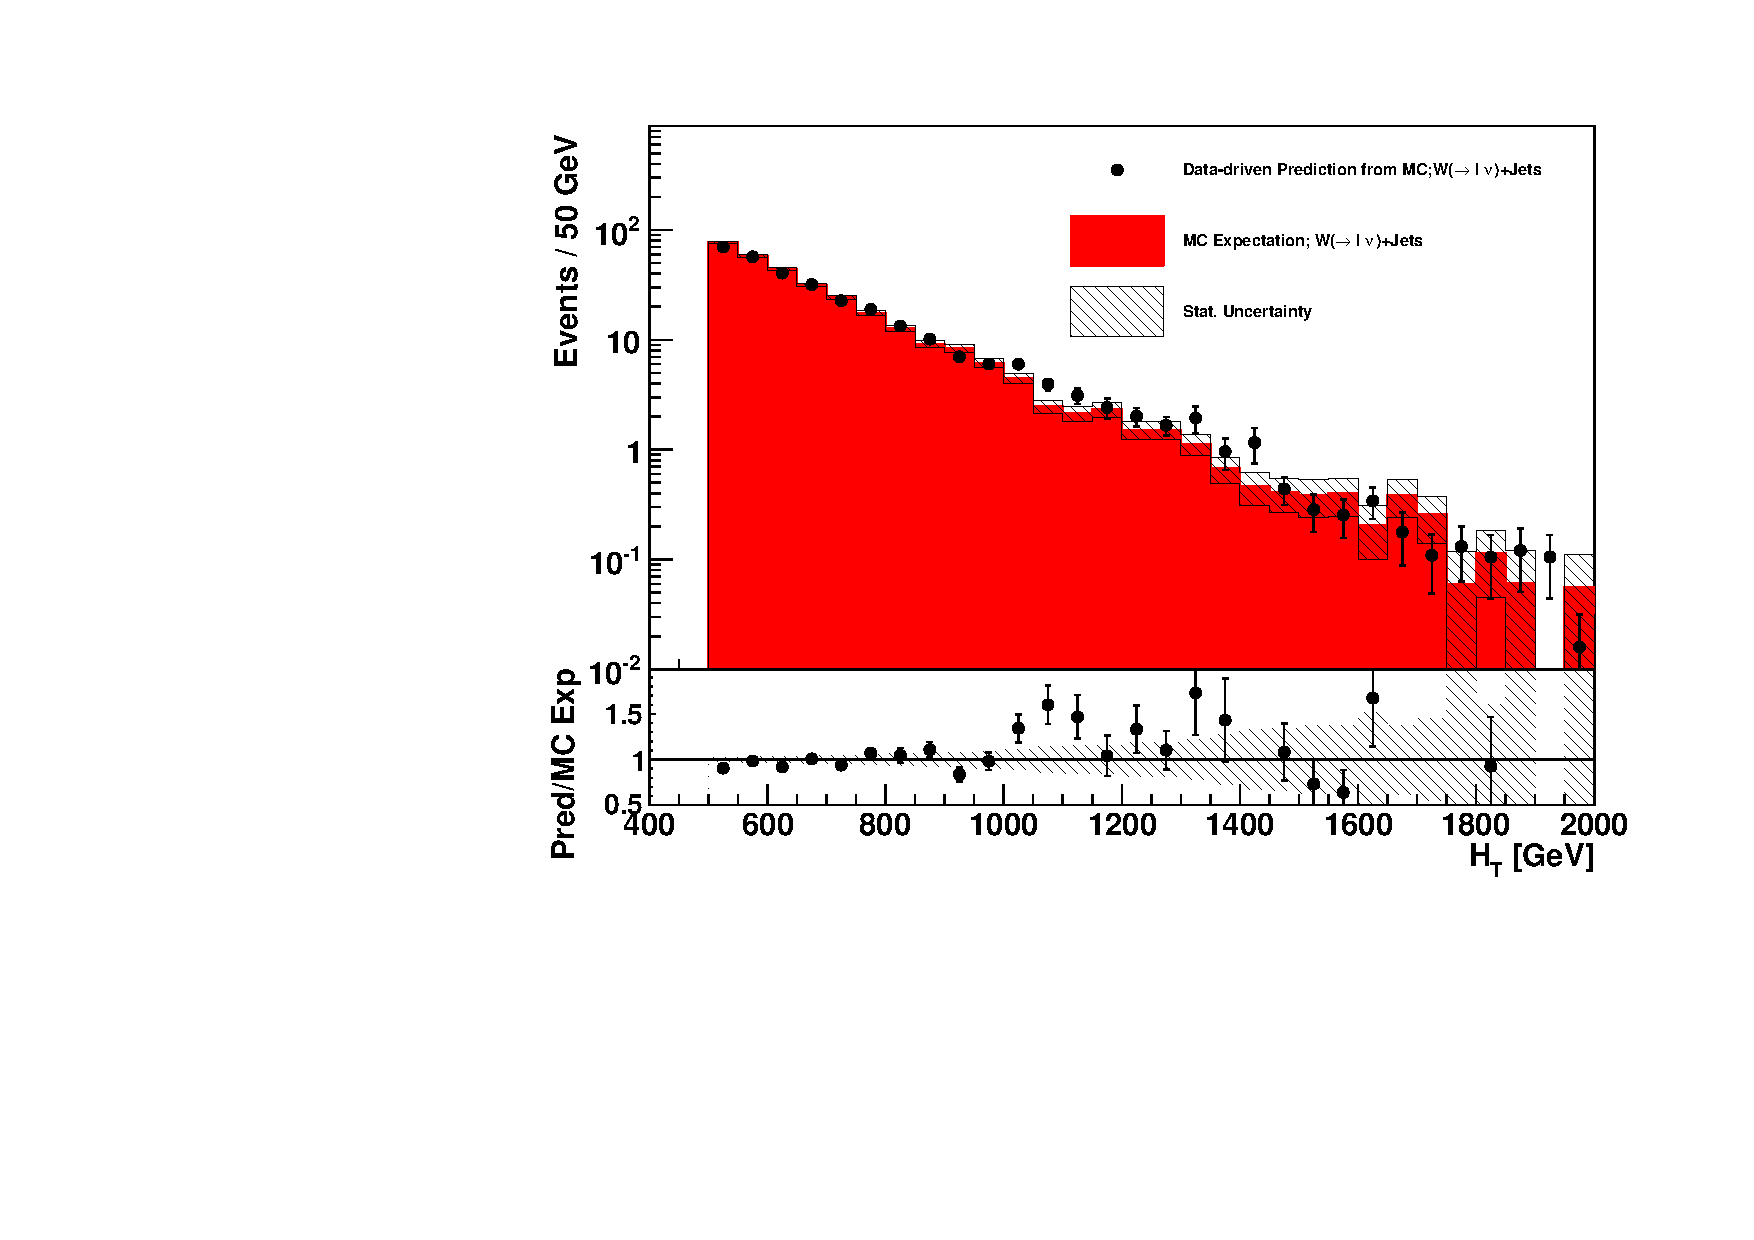
\includegraphics[width=0.90\textwidth]{lostlepton/plots/closure/HTw.pdf}\\
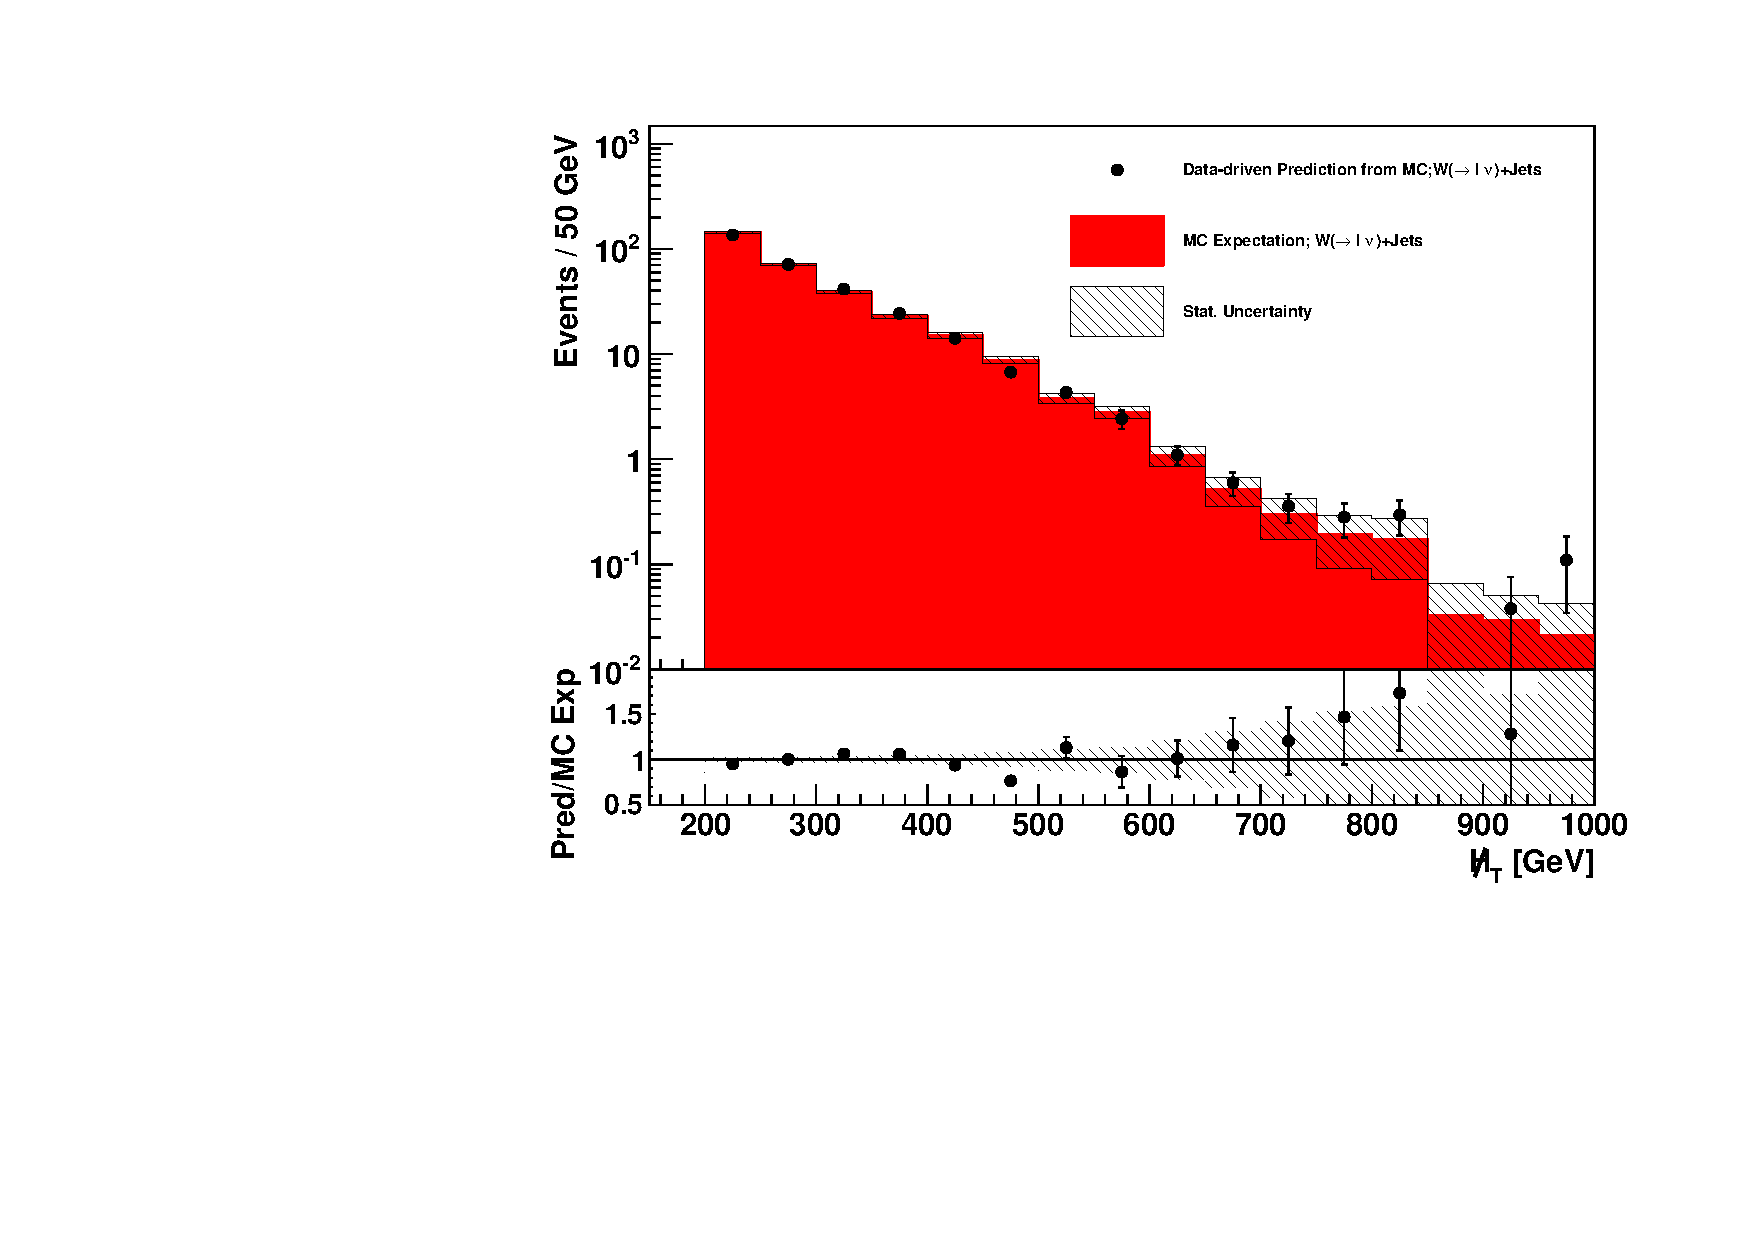
\includegraphics[width=0.90\textwidth]{lostlepton/plots/closure/MHTw.pdf}
%\includegraphics[angle=0,width=0.5\textwidth]{wtop_lostlepton_figures/MHTMHT_r}&
%\includegraphics[angle=0,width=0.5\textwidth]{wtop_lostlepton_figures/HTHT_r}
%%(a)&(b)\\
\end{tabular}
\end{center}
\caption{This plots show the closure test of the Data-driven Prediction from MC and the MC expectation for the \HT and \MHT distribution for \wpj simulated events. Good agreement of the shape as well as the ratio can be seen.}
\label{fig:closure_sepW}
\end{figure}





% ttbar MHT closure iso reco acc
\begin{figure}[tbhn]
\begin{center}
\begin{tabular}{cc}
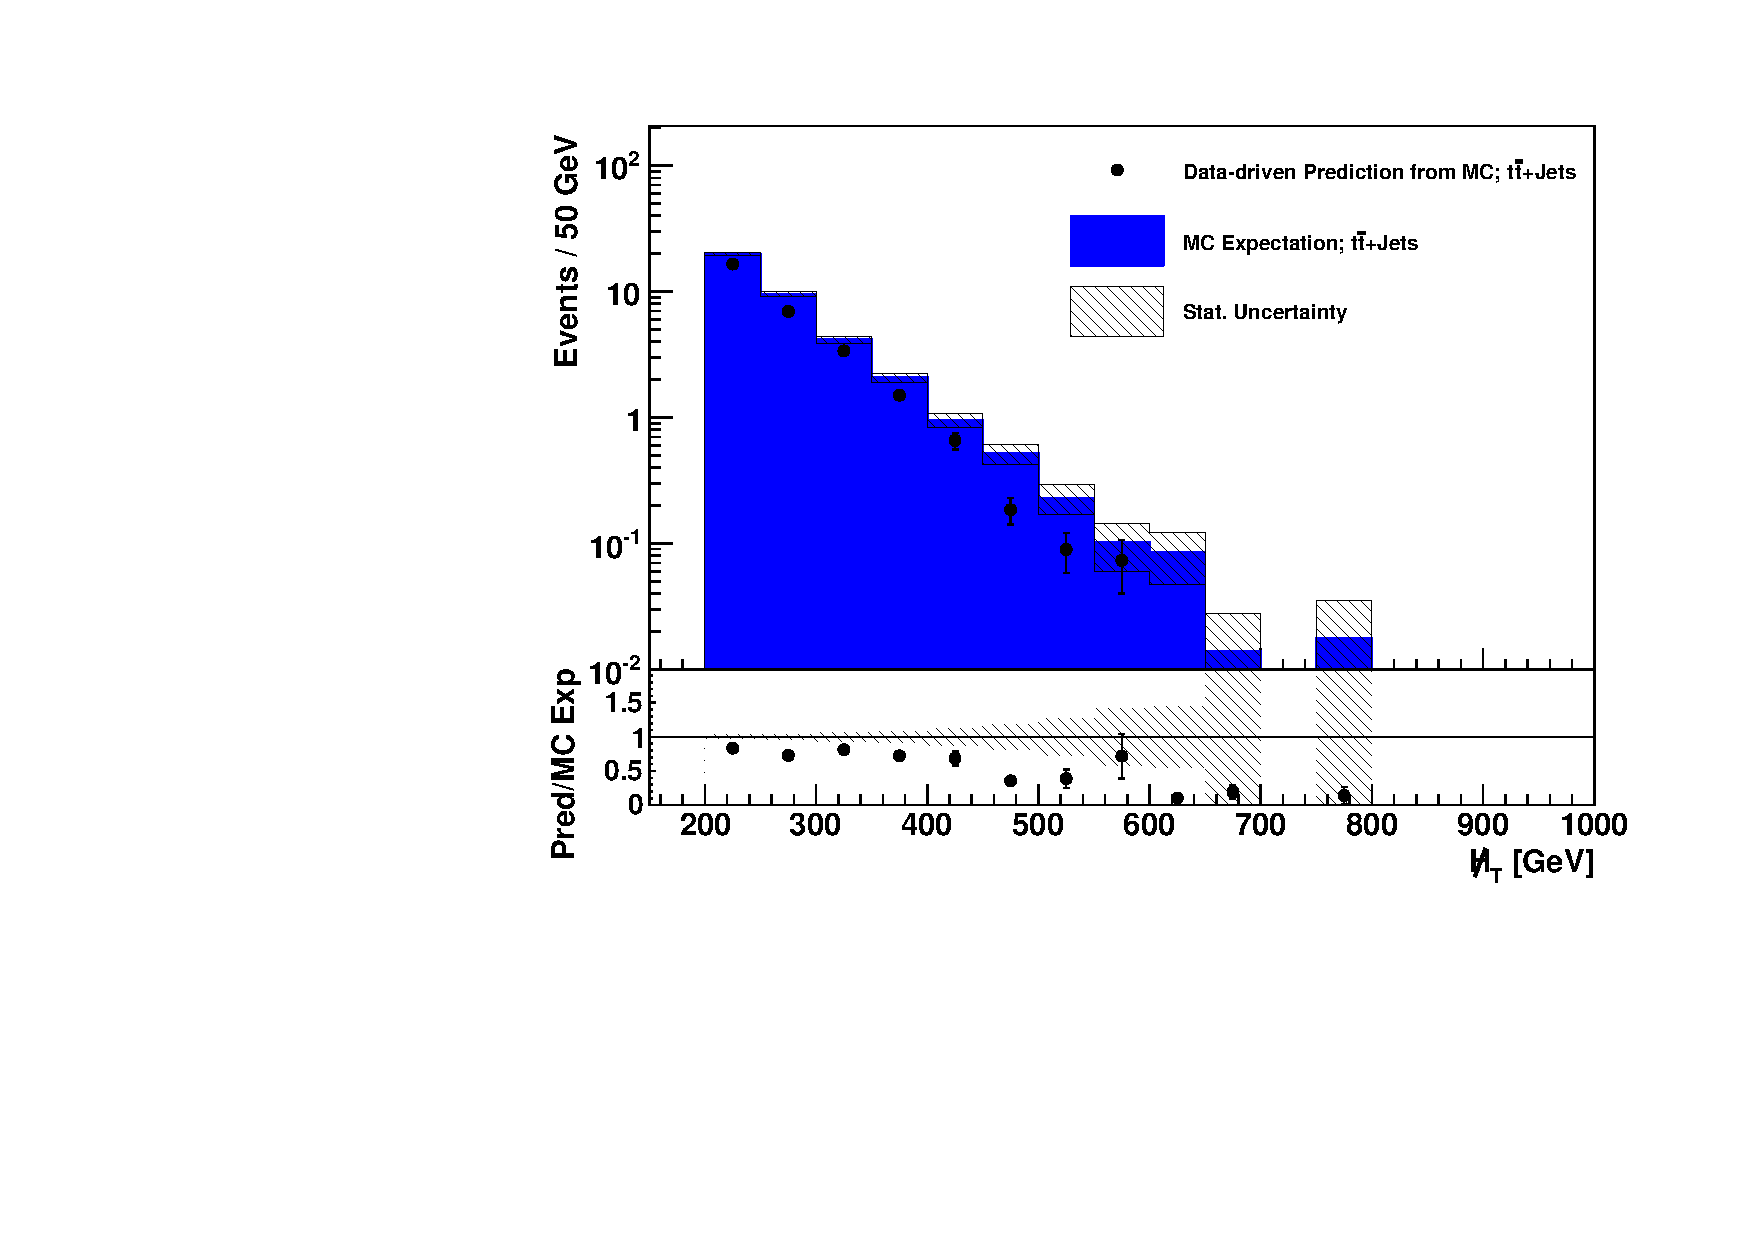
\includegraphics[width=0.50\textwidth]{lostlepton/plots/closure/MHTttbarIsoMu.pdf} 
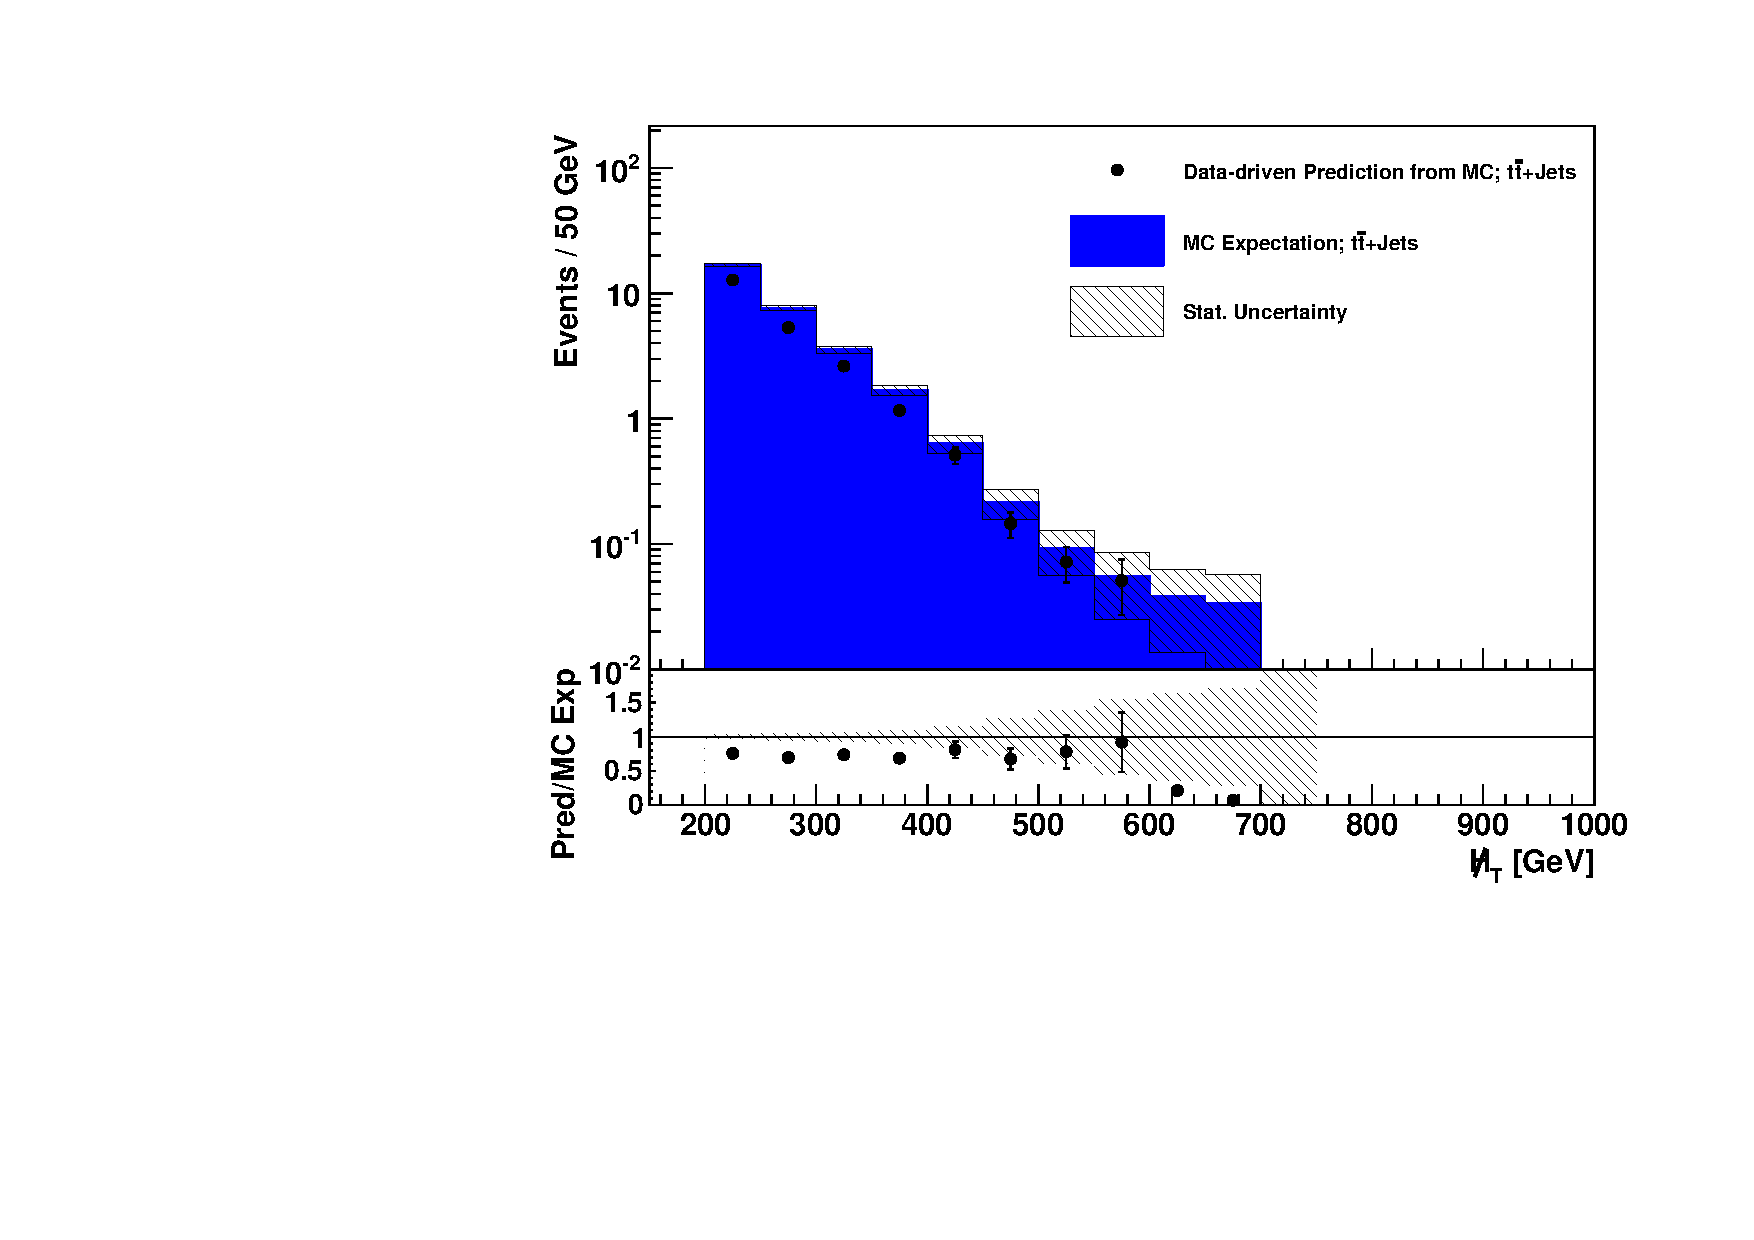
\includegraphics[width=0.50\textwidth]{lostlepton/plots/closure/MHTttbarIsoE.pdf} \\
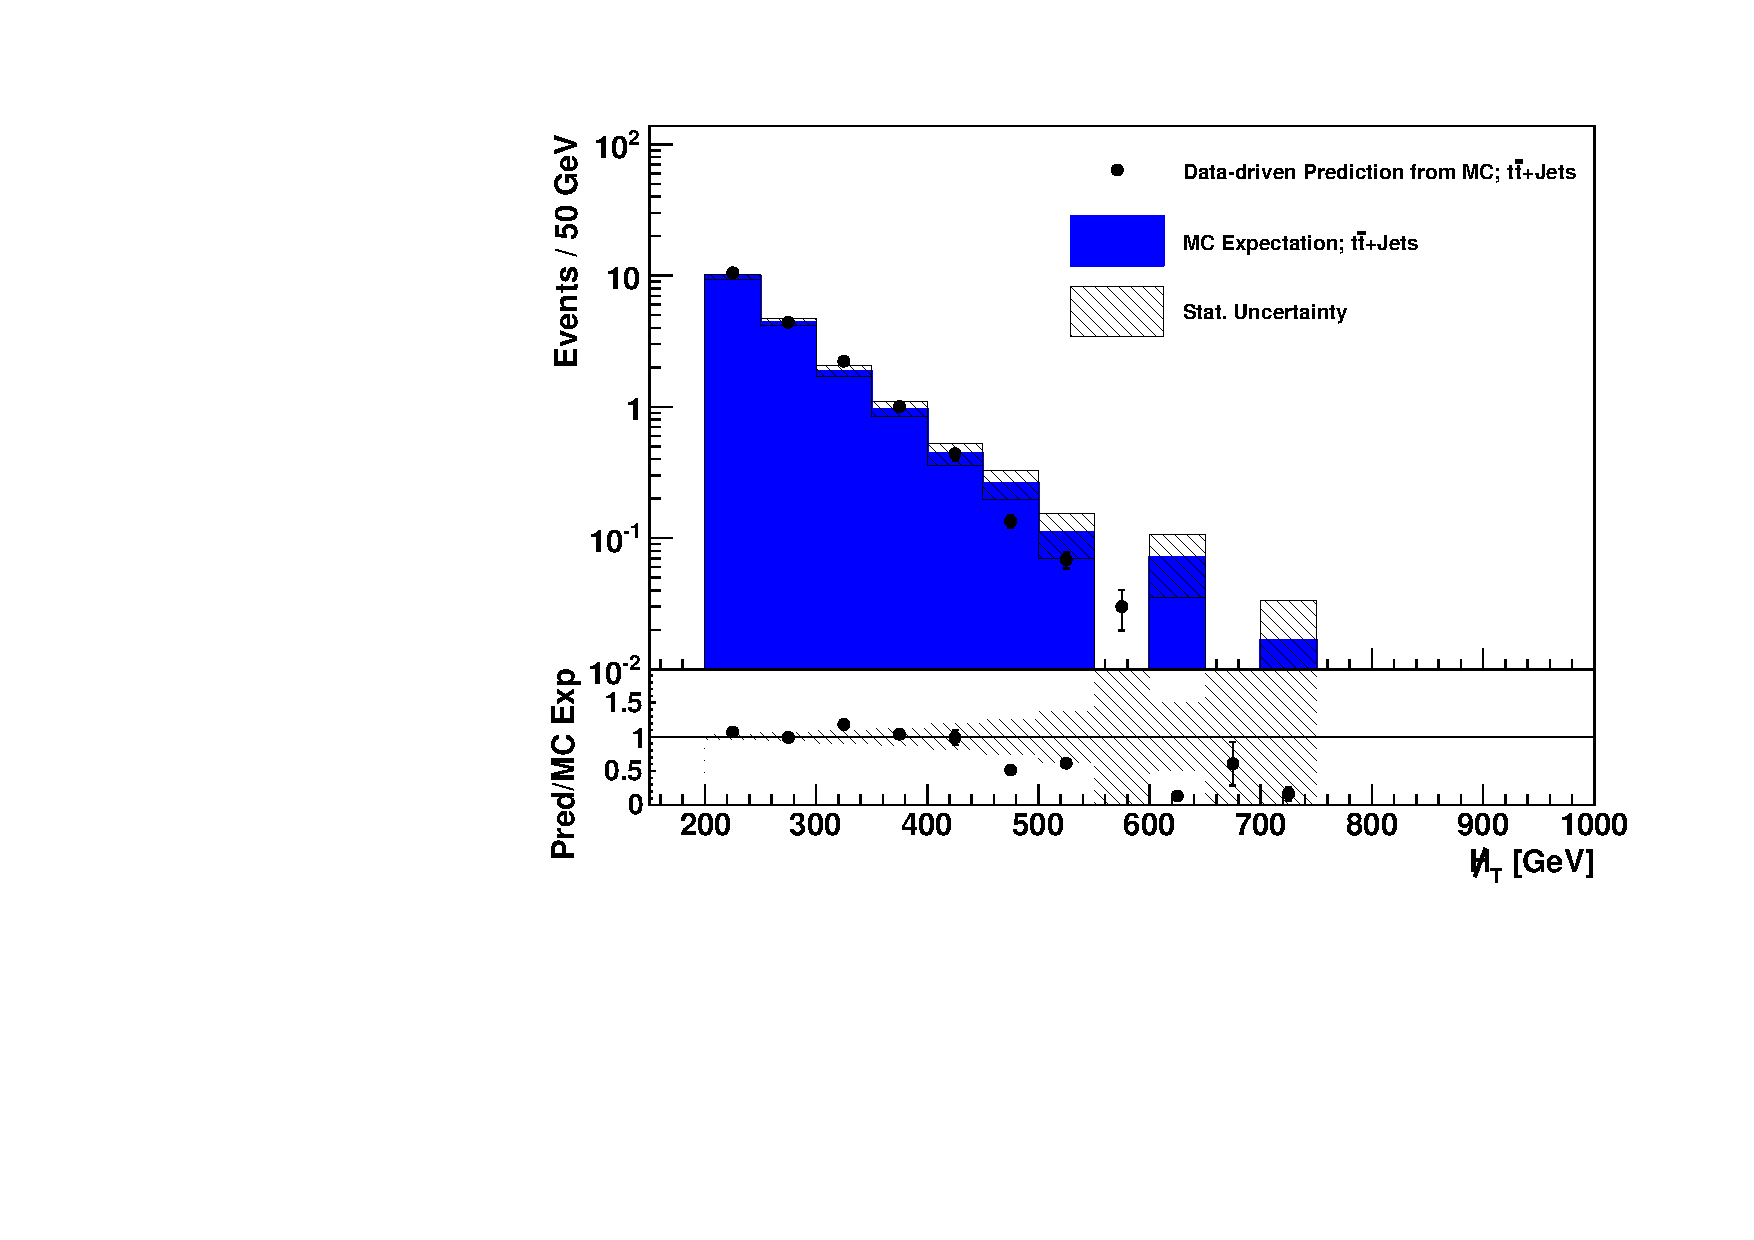
\includegraphics[width=0.50\textwidth]{lostlepton/plots/closure/MHTttbarRecoMu.pdf}
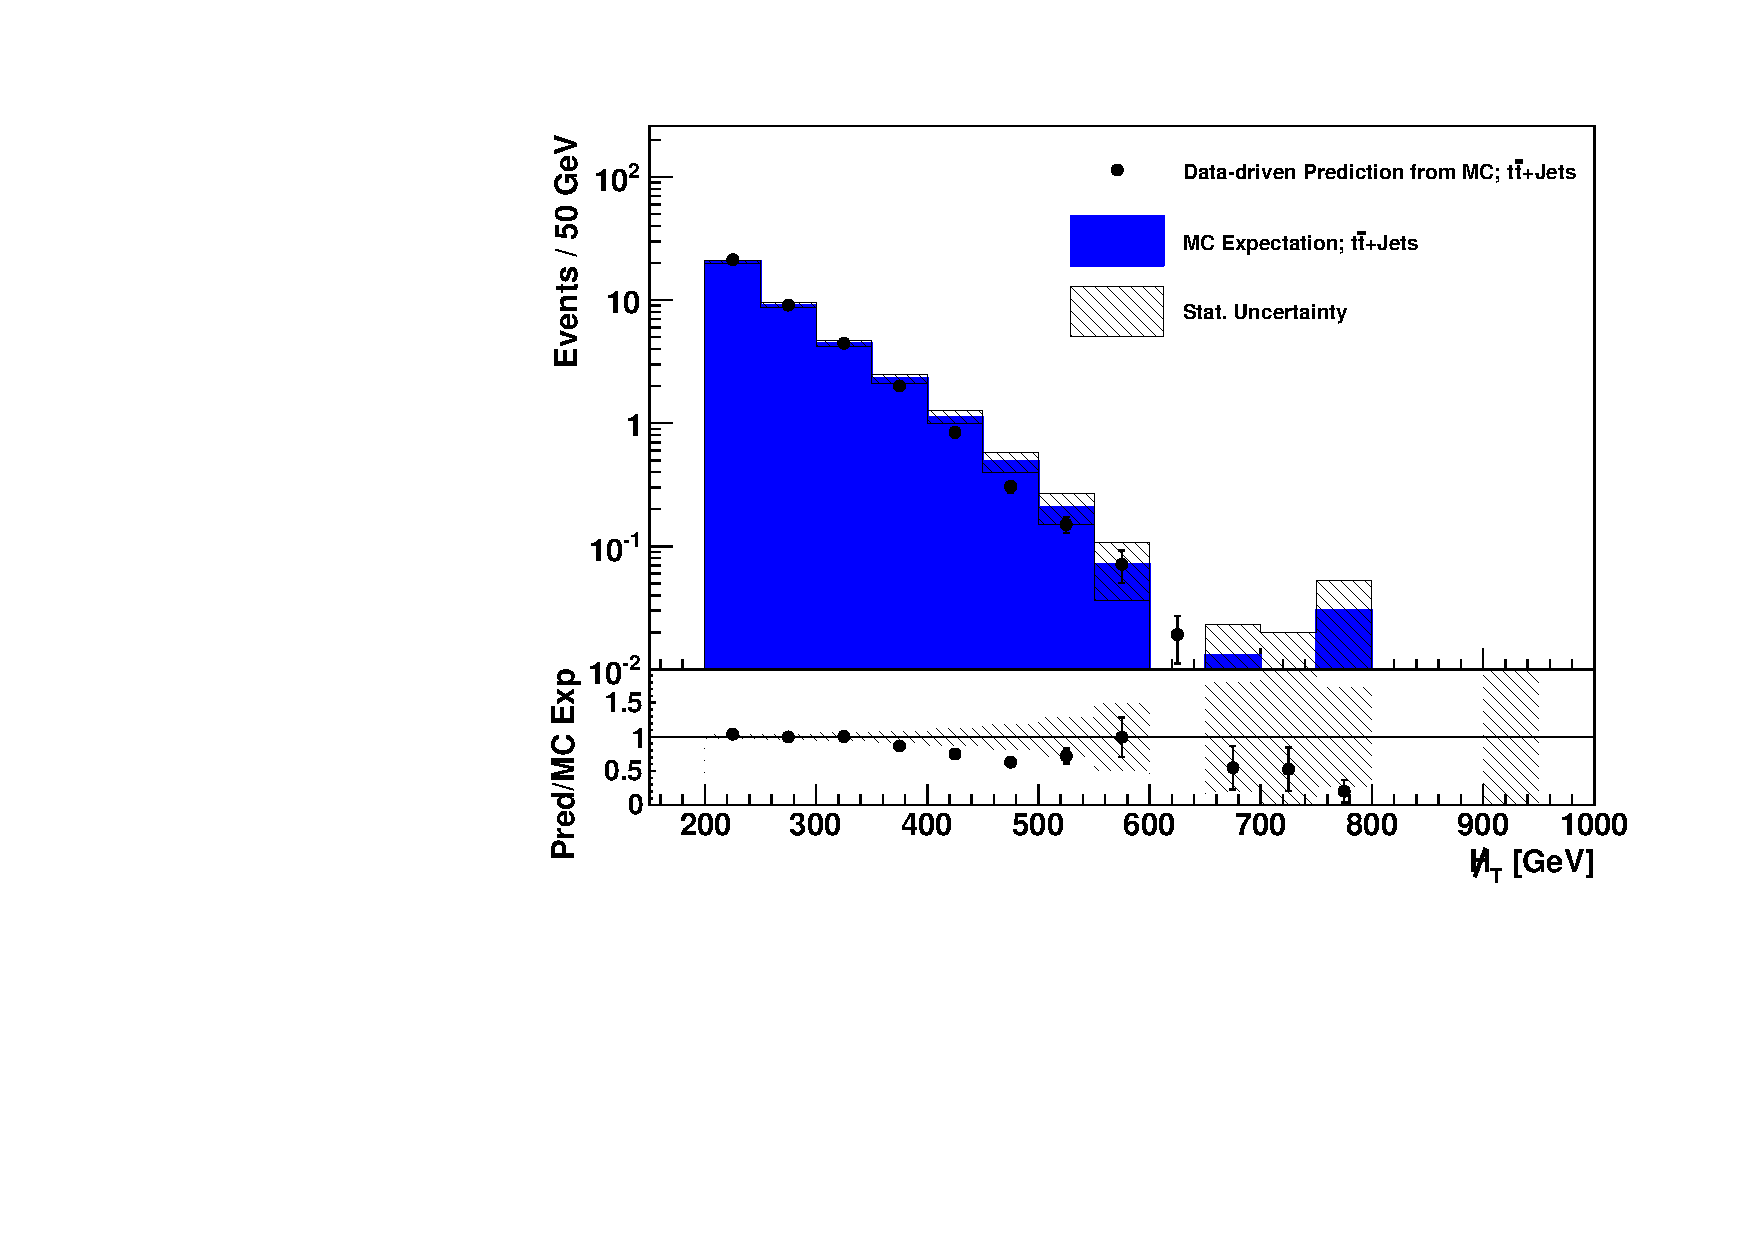
\includegraphics[width=0.50\textwidth]{lostlepton/plots/closure/MHTttbarRecoE.pdf}\\
\includegraphics[width=0.50\textwidth]{lostlepton/plots/closure/MHTttbarAccMu.pdf}
\includegraphics[width=0.50\textwidth]{lostlepton/plots/closure/MHTttbarAccE.pdf}\\
%\includegraphics[angle=0,width=0.5\textwidth]{wtop_lostlepton_figures/MHTMHT_r}&
%\includegraphics[angle=0,width=0.5\textwidth]{wtop_lostlepton_figures/HTHT_r}
%%(a)&(b)\\
\end{tabular}
\end{center}
\caption{This plots show the closure tests for \ttbar events separated for the not isolated (top), not reconstructed (middle) and out of acceptance fraction (bottom). Good agreement for the shape can be observed. However, an increasing under-prediction can also be seen. The legend description can be found in the caption of Fig.~\ref{fig:closure_sepTTbar}.
}
\label{fig:closure_ttbar_sep_MHT}
\end{figure}


% leading jet pt and number of jets
\begin{figure}[tbhn]
\begin{center}
\begin{tabular}{cc}
\includegraphics[width=0.50\textwidth]{lostlepton/plots/closure/MCClosureRecoMuMHT.pdf}
\includegraphics[width=0.50\textwidth]{lostlepton/plots/closure/MCClosureRecoEMHT.pdf}\\
\includegraphics[width=0.50\textwidth]{lostlepton/plots/closure/MCClosureAccMuMHT.pdf}
\includegraphics[width=0.50\textwidth]{lostlepton/plots/closure/MCClosureAccEMHT.pdf}\\
%\includegraphics[angle=0,width=0.5\textwidth]{wtop_lostlepton_figures/MHTMHT_r}&
%\includegraphics[angle=0,width=0.5\textwidth]{wtop_lostlepton_figures/HTHT_r}
%%(a)&(b)\\
\end{tabular}
\end{center}
\caption{The upper two plots show the closure test for the not reconstructed muon on the left and for electrons on the right for \ttbar and \wpj combined. On the bottom the same is shown for the out of acceptance background contribution. The legend description can be found in the caption of Fig.~\ref{fig:closure_sepTTbar}.
}
\label{fig:reco_acc_combined}
\end{figure}

\clearpage


 







% numbers of CS on data and MC



\begin{sidewaystable}[hbt]
%\fontsize{8 pt}{1.0 em}
\selectfont
\begin{centering}
\caption[]{Final event yield for the lost-lepton background for the exclusive search
regions. The numbers are for the full luminosity of \lumi. \label{tab:LostLeptonResult1}} 

\hspace*{-4ex}
\begin{tabular}{cc|c|c|c|c|c|c|c|c|c|c}
\HT (GeV)& \MHT (GeV)			& Pred. & Stat. & mu	 & MHT	& elec. 		& syst.		& acc 		& CS conta- 	 		& MTWcut 		& Tot.			\\
				&	& 	& 	& iso eff & fit	& iso eff		& eff	 	&  		& mination		&  			& Sys.			\\
\hline
baseline&			&	471.6	&27.3	&2.6	  &21.4	&$_{-2.7}^{+2.7}$	&47.2 		&16.2   	&$_{-14.1}^{+0.0}$	&$_{-19.6}^{+21.8}$	&$^{+58.6}_{-59.5}$	\\
\hline 
500\ldots 800& 200 \ldots 350		&323.7	&21.9	&1.6	  &14.8	&$_{-1.6}^{+1.6}$	&31.1 		&10.8   	&$_{-9.3}^{+0.0}$	&$_{-12.9}^{+14.4}$	&$^{+40.3}_{-40.9}$	\\
500\ldots 800& 350 \ldots 500		&47.4	&6.1	&0.1	  &3.9	&$_{-0.2}^{+0.2}$	&4.6 		&1.8    	&$_{-1.4}^{+0.0}$	&$_{-1.9}^{+2.1}$	&$^{+6.8}_{-6.8}$	\\	
500\ldots 800& 500 \ldots 600		&4.9	&2.0	&0.0	  &0.7	&$_{-0.0}^{+0.0}$	&0.5 		&0.2	   	&$_{-0.1}^{+0.0}$	&$_{-0.2}^{+0.2}$	&$^{+0.9}_{-0.9}$	\\
500\ldots 800& 600 \ldots		&0.8	&0.8	&0.0	  &0.2	&$_{-0.1}^{+0.1}$	&0.1 		&0.0	   	&$_{-0.0}^{+0.0}$	&$_{-0.0}^{+0.0}$	&$^{+0.2}_{-0.2}$	\\
\hline 
800\ldots 1000& 200 \ldots 350		&57.2	&13.4	&0.6	  &2.6	&$_{-0.5}^{+0.5}$	&5.5 		&1.6	   	&$_{-1.6}^{+0.0}$	&$_{-2.3}^{+2.5}$	&$^{+7.1}_{-7.2}$	\\
800\ldots 1000& 350 \ldots 500		&5.2	&2.1	&0.0	  &0.4	&$_{-0.0}^{+0.0}$	&0.5 		&0.2	   	&$_{-0.2}^{+0.0}$	&$_{-0.2}^{+0.2}$	&$^{+0.8}_{-0.8}$	\\
800\ldots 1000& 500 \ldots 600		&2.3	&1.3	&0.0	  &0.3	&$_{-0.0}^{+0.0}$	&0.2 		&0.1	   	&$_{-0.1}^{+0.0}$	&$_{-0.1}^{+0.1}$	&$^{+0.4}_{-0.4}$	\\
800\ldots 1000& 600 \ldots		&0.7	&0.7	&0.0	  &0.1	&$_{-0.0}^{+0.0}$	&0.1 		&0.0	   	&$_{-0.0}^{+0.0}$	&$_{-0.0}^{+0.0}$	&$^{+0.2}_{-0.2}$	\\
\hline 
1000\ldots 1200& 200 \ldots 350		&13.0	&3.3	&0.0	  &0.6	&$_{-0.1}^{+0.1}$	&1.3		&0.5	   	&$_{-0.4}^{+0.0}$	&$_{-0.5}^{+0.6}$	&$^{+1.7}_{-1.7}$	\\
1000\ldots 1200& 350 \ldots 500		&4.7	&4.1	&0.0	  &0.4	&$_{-0.0}^{+0.0}$	&0.5 		&0.1	   	&$_{-0.1}^{+0.0}$	&$_{-0.2}^{+0.2}$	&$^{+0.7}_{-0.7}$	\\
1000\ldots 1200& 500 \ldots		&1.5	&1.1	&0.0	  &0.3	&$_{-0.0}^{+0.0}$	&0.1 		&0.1	   	&$_{-0.0}^{+0.0}$	&$_{-0.1}^{+0.1}$	&$^{+0.3}_{-0.3}$	\\
\hline 
1200\ldots 1400& 200 \ldots 350		&4.0	&1.9	&0.0	  &0.2	&$_{-0.0}^{+0.0}$	&0.4 		&0.1	   	&$_{-0.1}^{+0.0}$	&$_{-0.2}^{+0.2}$	&$^{+0.5}_{-0.5}$	\\
1200\ldots 1400& 350 \ldots		&2.2	&1.3	&0.0	  &0.2	&$_{-0.0}^{+0.0}$	&0.2 		&0.1	   	&$_{-0.1}^{+0.0}$	&$_{-0.1}^{+0.1}$	&$^{+0.3}_{-0.3}$	\\
\hline 
1400\ldots& 200 \ldots			&2.6	&1.5	&0.0	  &0.2	&$_{-0.0}^{+0.0}$	&0.3 		&0.1	   	&$_{-0.1}^{+0.0}$	&$_{-0.1}^{+0.1}$	&$^{+0.4}_{-0.4}$	\\
\end{tabular}
\par\end{centering}
\end{sidewaystable}


\clearpage


\section{Pileup dependency studies}
\label{sec:pileup}
During the year 2011 the instantaneous luminosity increased. A consequence is that the so called pileup has increased. Pileup is defined as the amount of additional, usually soft, interactions per bunch crossing leading to additional primary vertices. Albeit this analysis is only interested in the hard interaction with large energy transfer, other interactions lead to additional activity and energy deposition in the detector which can interfere with the reconstruction of leptons and jets.\\
A good measurable quantity related to pileup is the number of primary vertices. The amount of primary vertices is proportional to the additional energy introduced by pileup events. Studies have been performed to investigate the possible dependence of the lost-lepton background estimation.\\
Possible sensitivity of this analysis on pileup is expected for the isolation or reconstruction efficiency. For the isolation criteria (see Eq.~\ref{eq:isolation} and Sec.~\ref{sec:event_selection}) the amount of momentum in the ECAL, HCAL and tracker close to the lepton is crucial. When pileup increases more particles are produced and the isolation efficiency is expected to decrease if the energy deposited by pileup is large compared to the energy of the leptons and jets.\\
Closure test in the number of vertices have been done for \ttbar and \wpj separately (see Sec.~\ref{sec:ll_prediction}) and closer tests for electrons and $\mu$ separately. The closure of the full MC reweighted to the full 2011 pileup scenario extracted from data is shown in Fig.~\ref{fig:pileup}. No dependency on the number of vertices can be observed. Plot~\ref{fig:pileup_iso} shows the the closure test for the number of primary vertices for the not isolated electrons and muons for \ttbar and \wpj separately. If any of the estimations would depend significantly on pileup an increasing under-prediction would be expected with increasing number of vertices. The samples for both electrons and muons show no such dependency, thus the isolation is not affected considerably by the pileup here studied. For the out of acceptance leptons no dependency is expected which is demonstrated in Fig.~\ref{fig:pileup_acc}).
\begin{figure}[tbhn]
\begin{center}
\begin{tabular}{cc}
\includegraphics[width=0.90\textwidth]{lostlepton/plots/ANplots/Closure_NVertex.pdf}
\end{tabular}
\end{center}
\caption{This plot shows the closure test for the \ttbar and \wpj MC combined as a function of the number of primary vertices. The MC was reweighted according to the full 2011 pileup scenario. The legend description can be found in the caption of Fig. \ref{fig:closure}}
\label{fig:pileup}
\end{figure}
\begin{figure}[tbhn]
\begin{center}
\begin{tabular}{cc}
\includegraphics[width=0.49\textwidth]{lostlepton/plots/closure/NVttbarIsoE.pdf}
\includegraphics[width=0.49\textwidth]{lostlepton/plots/closure/NVttbarIsoMu.pdf}\\
\includegraphics[width=0.49\textwidth]{lostlepton/plots/closure/NVwIsoE.pdf}
\includegraphics[width=0.49\textwidth]{lostlepton/plots/closure/NVwIsoMu.pdf}\\
\end{tabular}
\end{center}
\caption{These plots show the closure test for the number of primary vertices separated for not isolated muons (left) and not isolated electrons (right), for \ttbar (top), and \wpj (bottom). The method shows no dependency on the number of vertices neither for \ttbar nor for \wpj events. The legend description can be found in the caption of Fig.~\ref{fig:closure_sepTTbar}.}
\label{fig:pileup_iso}
\end{figure}
\clearpage
The same studies were done to check if the reconstruction efficiencies have any pileup dependency. Fig.~\ref{fig:pileup_reco} shows a similar closure test for the not reconstructed muons and electrons, again no dependency on increasing pileup is being observed.
\begin{figure}[tbhn]
\begin{center}
\begin{tabular}{cc}
\includegraphics[width=0.49\textwidth]{lostlepton/plots/closure/NVttbarRecoE.pdf}
\includegraphics[width=0.49\textwidth]{lostlepton/plots/closure/NVttbarRecoMu.pdf}\\
\includegraphics[width=0.49\textwidth]{lostlepton/plots/closure/NVwRecoE.pdf}
\includegraphics[width=0.49\textwidth]{lostlepton/plots/closure/NVwRecoMu.pdf}\\
\end{tabular}
\end{center}
\caption{The two upper plots show the closure test for the not reconstructed electrons (right) and muons (left) for \ttbar as the number of vertices while the two lower plots show the same distribution but for the \wpj sample. The legend description can be found in the caption of Fig.~\ref{fig:closure_sepTTbar}.}
\label{fig:pileup_reco}
\end{figure}
For the out of acceptance fraction no pileup dependency is expected. The \pt of the muons and electrons does not depend on the activity in the detector and also the amount of leptons out of the geometrical acceptance of the detector is not influenced by pileup.\\%(see the out of acceptance closure plots in the appendix \ref{appendix:OutAcceptancePLots} 
As is shown and discussed above no contribution of the prediction shows any dependency on the number of vertices. The isolation criteria is very lose with a small cone and the selection requires already high energy. This justifies the statement that for the pileup here studied reaching out to about 16 number of vertices with reasonable statistics the lost-lepton background prediction is not significantly influenced by pileup.\\
For the even further increase in pileup, which is expected during data taking 2012, studies on MC samples simulated with higher pileup are needed. 

\clearpage

\section{PDF uncertainties on the acceptance}
\label{sec:pdf}
The method which has been used to estimate the PDF uncertainties is described in \cite{Bourilkov:2006cj}.
In general parton distribution functions (PDF) are measured quantities with uncertainties. PDFs provide the probability $F_{i}=F(x_{i},Q)$ of finding a parton $i$ with the longitudinal momentum fraction $x$ and the momentum transfer $Q$ in a proton or antiproton.
The PDFs come into play when the cross-section of a process involving protons (Eq.~\ref{eq:pdfCross_section}) is calculated:
\begin{equation}
\frac{d\sigma}{d \xspace variable} [pp \rightarrow X] \sim \sum_{ij} (f_{i/p}(x_{1})f_{j/p}(x_{2})+(i\leftrightarrow j))\hat \sigma
 \label{eq:pdfCross_section}
\end{equation}
%%$\hat\sigma$
$\hat \sigma \xspace$ -  cross section for the partonic subprocess $ij\rightarrow X$, \\
$x_{1}x_{2} \xspace $ - parton momentum fraction, \\
$f_{i/p}(x_{i}) \xspace $ - probability to find a parton $i$ with momentum fraction $x_{i}$ in the proton.\\
\vspace*{3mm}
It is now necessary to understand how the PDF uncertainty contributes to the uncertainty of the probability of a process. The PDF uncertainties are obtained from of a set of N Eigenvectors \footnote{$N=20$ for CTEQ6 which has been used here} which have been orthogonalized with the Hessian Method. Each eigenvector probes a direction in the PDF parameter space that is a combination of the $N$ free parameters used in a global fit on measured data. To calculate the uncertainty, the $N$ eigenvectors have to be varied.
Each eigenvector is varied up and down within tolerance to obtain $2N$ new parameter sets. By construction the variation in the direction of such eigenvectors is symmetric but this is not necessarily true when the uncertainties are propagated to the observable which depends on all $N$ eigenvalues. To calculate the uncertainty the so called ''Master Equation''\cite{Bourilkov:2006cj} has been used:

\begin{equation}
 \Delta X_{max}^{+}=\sqrt{\sum_{i=1}^{N}[\text{max}((X_{i}^{+})-(X_{0}),(X_{i}^{-})-(X_{0},0))]^{2}}
\label{eq:MasterEquation1}
\end{equation}
\begin{equation}
 \Delta X_{max}^{-}=\sqrt{\sum_{i=1}^{N}[\text{max}((X_{0})-(X_{i}^{+}),(X_{0},0)-(X_{i}^{-}))]^{2}}
\label{eq:MasterEquation2}
\end{equation}
with $X_{i}^{\pm}$ being the up and down variation of the $i$ Eigenvector with the mean $X_0$ for the physical observable $X$. 
To obtain the PDF uncertainty on the acceptance the variation of the in and out of acceptance leptons needs to be calculated. This has been done according to the PDF4LHC recommendation with a tool provided by the Electroweak group \cite{electroweak:2010}.
The uncertainty for \ttbar and \wpj events have been calculated separately because for the \ttbar events a much higher uncertainty is expected since for the production gluon fusion is dominant where for \wpj, quark-quark interaction is mainly responsible. The gluon distribution in the proton can only be measured indirectly which results in bigger uncertainties compared to the direct measurable quark distribution\cite{bib:HERA:pdf}.
The CETQ66 PDF sets\cite{bib:cteq:web} were used to generate the studied MC samples (Sec.~\ref{sec:samples}).\\
The resulting uncertainty on the acceptance efficiencies have been found to be 5.4\% up and 4.7\% down for the \ttbar sample and 2.0\% up and 2.1\% down for the \wpj sample. Together with the uncertainty on the ratio between \wpj and \ttbar events, discussed above (Sec.~\ref{sec:uncertainties}) a $6\%$ uncertainty on the prediction has been applied. 




\section{Uncertainties}
\label{sec:uncertainties}

This section discusses how the most relevant uncertainties were found and justified. Tab.~\ref{tab:uncertainties} includes all contribution that make up the total uncertainty for the baseline selection.
\begin{table}[tbn]
\caption{The dominating systematic uncertainties of the lost-lepton prediction for the baseline selection.} 
\begin{center}
\begin{tabular}{lll|rr}
                    &\multicolumn{2}{c}{} \\\hline
 \# &Source &\multicolumn{3}{|c|}{Systematic Uncertainties} \\\hline
 1	&Statistics of the control-sample                & $+4.3\%$ & $-4.3\%$\\
 2	&iso-efficiencies (statistical, fit)   	         & $+5.6\%$ & $-4.1\%$\\
 3	&Differences $t\bar{t}$, \wpj, $Z$-samples        & $+10.0\%$ & $-10.0\%$\\
 	&and kinematic in control vs. signal region      &  & \\
 4	&Possible \MHT dependency		         & $+4.5\%$ & $-4.5\%$\\
 5	&SM background in control-region                 &    $+0\%$ & $-3.0\%$ \\
 6	&MC use for acceptance calculation               & $+3.9\%$ & $-3.9\%$\\
 7	&transverse W-mass-cut			         & $+4.6\%$ & $-4.0\%$ \\
\hline
	&total, combined systematics                     & $+13.1\%$  & $-13.9\%$\\
\hline
 \end{tabular}
\end{center}
\label{tab:uncertainties}
\end{table}
The difference of the \ttbar, \wpj and $Z$ sample, the SM background in the control-region, MC use for acceptance calculation and the \mt cut are constant for all search regions while the statistics of the CS, the isolation efficiencies and the possible \MHT dependency are calculated for each region individually.
The following enumeration corresponds to Tab.~\ref{tab:uncertainties}.

\begin{enumerate}
 \item The most obvious uncertainty is the statistical uncertainty on the CS, $S_{CS}=\sqrt{\sum_i{w_i}}$ with $S_{CS}$ being the statistical uncertainty and $w_i$ the weight (calculated according to Eq.\ref{eq:totalWeight} divided by CS) of each event in the CS. 

 \item The isolation efficiencies for electrons and muons have been measured by a Tag\&Probe method (see Sec.~\ref{sec:tag_probe}) on a $Z$-sample were the $Z$ decays leptonically. The uncertainty arising from the statistical limitation on this sample and the error due to to the fitting procedure have been taken into account.

 \item
 The electron and muon reconstruction efficiencies have been obtained from MC. The fraction of events including not reconstructed electrons and muons contribute $24\%$ to the total background. An  uncertainty of $9\%$ on the total prediction has been found to be conservative by comparing the used MC efficiencies with the old Tag\&Probe efficiencies. Together with other systematic uncertainties related to kinematic differences of the control- and signal region, as well as to remaining sample dependencies of the parametrized lepton efficiencies that are obtained on a $Z$-samples and applied to the \ttbar and \wpj samples, an uncertainty of 10\% is applied. 

 \item Fig.~\ref{fig:closure_ttbar_sep_MHT} shows the closure test for the \MHT distribution of the not isolated muons (among other) for \ttbar events (\wpj see Fig.~\ref{fig:closure_w_sep_MHT}). With increasing \MHT an increasing under-prediction is being observed. As discussed in Sec.~\ref{sec:isolation} the efficiency can not account for this. Fig.~\ref{fig:LostLeptonMHTfit} shows the relative difference between Data-driven Prediction from MC and MC expectation with a constant fit (red line) together with an blue error band which corresponds to the envelop of the the maximum of a linear fit $\pm1$ sigma error relative to the constant fit. The blue uncertainty band is taken as additional uncertainty on the prediction. The \MHT selection for each exclusive search region determines the applied uncertainty. Tab.~\ref{tab:LostLeptonSlope} shows these uncertainty for each \MHT selection. 
This \MHT dependency and possible others are treated as an additional uncertainty of up to 20\% on the prediction. 

% MHT Fit
\begin{figure}[tbhn]
\begin{center}
\begin{tabular}{c}

\includegraphics[width=0.90\textwidth]{lostlepton/plots/MHT_fit2.pdf}
%\includegraphics[angle=0,width=0.5\textwidth]{wtop_lostlepton_figures/Prediction_HT.pdf} &
%\includegraphics[angle=0,width=0.5\textwidth]{wtop_lostlepton_figures/Prediction_MHT.pdf} \\
\end{tabular}
\end{center}
\caption{This plot shows the relative difference between Data-driven Prediction on MC and MC Expectation (dots with error band). Also a fit with a constant is shown(red). The blue lines show the $\pm$ 1 sigma envelope of a linear fit relative to the constant fit.}
\label{fig:LostLeptonMHTfit}
\end{figure}


 \item Background events from QCD, $Z$- or diboson events have been investigated by selecting a control sample on corresponding MC samples (see Sec.~\ref{sec:other_sm_contribution}). Since only a very small number of events has been found to contribute a conservative uncertainty of $3\%$ is adopted (see Sec.~\ref{sec:other_sm_contribution}).

 \item The corrections for out-of-acceptance leptons have been taken from MC. The uncertainty on the acceptance efficiency is found to be smaller than 9\% leading to a total uncertainty of about 6\% on the prediction. This value covers the PDF uncertainty discussed in greater detail in Sec.~\ref{sec:pdf} and the uncertainty on the different contribution of the \ttbar and \wpj sample.


 \item A minor contribution to the total statistical uncertainty arises from the correction due to the transverse mass cut discussed in Sec.~\ref{sec:signal_contamination}. This uncertainty can be divided into three parts:\\
\begin{itemize}
 \item The \met scale dependence, which has been determined by observing the variation of the correction factor while varying the \met by 10\%,
 \item a conservative assumption on the uncertainty due to \met outliers\footnote{\met outliers arise when },
 \item and an uncertainty on the fraction of dileptonic \ttbar events which has been obtained from MC.
\end{itemize}
 The correction factor with the combined uncertainty is calculated to be $10\% \pm 4\%$. Studies have been performed (see Sec.~\ref{sec:signal_contamination}) on the efficiency of the \mt cut for each search region. The variation of the mean of the  efficiency is within the 40\% assigned uncertainty.
 
\end{enumerate}



\begin{table}[hbt]
\fontsize{10 pt}{1.2 em}
\selectfont
\begin{centering}
\caption[]{This table contains the uncertainty assigned according to the \MHT selection of each region due to \MHT decency of the prediction.\label{tab:LostLeptonSlope}} 
\hspace*{-4ex}
\begin{tabular}{c|c}
\MHT (GeV)			& Pred. \\
\hline 
200 \ldots 350		&4.6\% \\
200 \ldots		& 8.2\%    \\
350 \ldots 500		&8.2\% \\	
350 \ldots		&8.2\% \\
500 \ldots 600		&13.3\%  \\
500 \ldots		&16.4\%   \\
600 \ldots		&20.0\%  \\

\end{tabular}
\par\end{centering}
\end{table}
\clearpage



